\begin{chapter}{Spawning in non-adiabatic crossings}
\label{ch:spawncrossbasics}


In the following chapter we try to use the ideas on spawning wavepackets in the
case of a non-adiabatic potential with several energy levels. First we will
look at the theoretical side and show how to use the formulae derived in chapter
\ref{ch:spawnprocedure}. We will see that this is straight forward and results
in formulae with a structure well known from above. Later we recover
algorithms similar to the ones from the last chapter. They are not necessarily
more general but rather put the focus onto other points.

The second part of this chapter is used to show some simulation results in great
detail and demonstrate the capabilities of the spawning algorithms. We will
see how the until then theoretical spawning ideas perform in
practice. The potential has only two energy levels and one single avoided
crossing in the middle. This is probably the simplest example we could use
for testing but already here we will discover several interesting facts.
The results are mostly good but not without some smaller challenges.

We perform aposteriori spawning only, the reason for this is that the
propagation spawning in the non-adiabatic case is considerable more complicated
than in the tunneling examples. But an algorithm adapted to the special case of
our simulations with only a single avoided crossing is given at the end.

The generalized algorithms for arbitrary potentials with an arbitrary number
of energy levels and many crossings will be sketched in the next chapter.


\section{Adapting the theoretical basis}
\label{sec:theoretical_basis_na}

The theory presented in chapter \ref{ch:spawnprocedure} is general enough that
we can use it to describe parameter estimation and the change of basis
also in the case of non-adiabatic potentials. In this case we have a potential
$V\ofs{x}$ with $N$ energy levels denoted by $\lambda_0 ,\ldots, \lambda_{N-1}$ and the
wavepacket $\Ket{\Psi}$ has $N$ different components $\Phi_0, \ldots, \Phi_{N-1}$
too. Assume for the moment that all wavepackets are homogeneous ones. (We can drop
this requirement at any time but have to be careful with the individual parameter
sets $\Pi_i$ for each component $\Phi_i$.)

The ideas of spawning packets and therewith replacing parts of already existing
packets now apply not to subsets of $\Phi_0$ like in the tunneling case but
to \emph{whole} components $\Phi_i$. To clarify this let's make a small example
and assume our $\Psi$ is defined as $\Psi \assign \left(\Phi_0=\phi_0, \Phi_1=0\right)$
where we have a $\phi_0$ on the first component and nothing on the second. If
we propagate this packet through an avoided crossing then there will appear
another fragment $w$ on the lower level whose shape depends mainly on the incoming packet
and on the gap size $\delta$. So after the crossing our wavepacket looks like
$\Psi^\prime = \left(\Phi_0=v, \Phi_1=w\right)$ where $v$ and $w$ are some
linear combinations of basis functions. (We omitted the global phase in this
example.) If now the parts $v$ and $w$ propagate at different speed it is
a bad idea to keep them glued together in the same wavepacket $\Psi^\prime$.
The reason is similar to what we gave as motivation for developing the spawning
ideas in the first place. We will need a basis with more and more high frequency
parts although both packets have (for example) the shape of a Gaussian. The idea
to split of one of the two parts $v$ or $w$ and put it into a new wavepacket now
arises naturally.

To go back from this small example to the general case, we assume that we want
to split of the wavefunction represented by the component $\Phi_\nu$ where
$\nu=1$ above and $\nu \in [0, N-1]$ in general. We call $\nu$ the index of
the \emph{monitored component}. For now presume the $\nu$
is given and we do not have to find it. The fragment for which we perform
the parameter estimation is now the whole component $\Phi_\nu$ and we
write $w \assign \Phi_\nu$ and return to chapter \ref{ch:spawnprocedure} to
see what this implies. First of course it tells us the values for $\alpha$
and $\beta$, namely $\alpha=0$ and $\beta=K-1$ where $K$ is the basis size
of $\Phi_\nu$. This is already enough to simplify the two formulae
\eqref{eq:estimate_pos} and \eqref{eq:estimate_mom} for position and momentum
estimation. By plugging in the values we get

\begin{align}
  \tilde{q} & \assign \frac{\Braket{w | x | w}}{\Braket{w|w}}
            = \frac{\sqrt{2 \varepsilon^2}}{\sum_{k=0}^{K-1} \conj{c_k} c_k} \Re \left(Q \sum_{k=1}^{K-1} \conj{c_k} c_{k-1} \sqrt{k} \right) + q
            \label{eq:estimate_pos_na} \\
  \tilde{p} & \assign \frac{\Braket{w | y | w}}{\Braket{w|w}}
            = \frac{\sqrt{2 \varepsilon^2}}{\sum_{k=0}^{K-1} \conj{c_k} c_k} \Re \left(P \sum_{k=1}^{K-1} \conj{c_k} c_{k-1} \sqrt{k} \right) + p \,.
            \label{eq:estimate_mom_na}
\end{align}

For the second moments we apply the same simplifications to \eqref{eq:est_second_moment_pos_final}
and \eqref{eq:est_second_moment_mom_final} and get

\begin{align} \label{eq:est_second_moment_pos_na}
  \frac{\Braket{w|\left(x-\tilde{q}\right)^2|w}}{\Braket{w|w}} & =
  \frac{
    \varepsilon^2 \Re \left( Q^2 \sum_{k=0}^{K-3} \conj{c_{k+2}} c_{k} \sqrt{k^2+3k+2} \right)
    + \frac{\varepsilon^2}{2} |Q|^2 \sum_{k=0}^{K-1} \conj{c_k} c_k \left(2k+1\right)
  }{\sum_{k=0}^{K-1} \conj{c_k} c_k}
  - \left(q - \tilde{q}\right)^2 \,.
  \\ \label{eq:est_second_moment_mom_na}
  \frac{\Braket{w|\left(x-\tilde{p}\right)^2|w}}{\Braket{w|w}} & =
  \frac{
    \varepsilon^2 \Re \left( P^2 \sum_{k=0}^{K-3} \conj{c_{k+2}} c_{k} \sqrt{k^2+3k+2} \right)
    + \frac{\varepsilon^2}{2} |P|^2 \sum_{k=0}^{K-1} \conj{c_k} c_k \left(2k+1\right)
  }{\sum_{k=0}^{K-1} \conj{c_k} c_k}
  - \left(p - \tilde{p}\right)^2 \,.
\end{align}

These four equations are all we need to estimate the parameters $\tilde{q}$, $\tilde{p}$,
$\tilde{P}$ and $\tilde{Q}$ of our fragment $w = \Phi_\nu$. In contrast to the tunneling
case we can in general \emph{not} set $k=0$ in \eqref{eq:estimate_abssqrPQ} and have
to keep the variable $k$ as an input parameter of our algorithm. In the simulations later
in this chapter therefore we also show the same simulation setups with different values
of $k$. The remainder of the overall spawning process works as described in chapter
\ref{ch:spawnprocedure} and especially the two algorithms for changing the basis
from $\Pi$ to $\tilde{\Pi}$ stay the same but take as input $w = \Phi_\nu$. Both
algorithms are still valid but we will use almost exclusively the basis projection
because is is much more flexible and error tolerant and we hardly ever have a pure
$\phi_i$ on the component $\Phi_\nu$.


\section{Basic avoided crossings simulations}

In this section we present the simulations that are used as the base for later
aposteriori spawning simulations. The potential has a single avoided crossing
and is shown in figure \ref{fig:avoided_crossing}. We will start with different
initial wavepackets $\Ket{\Psi}$ on the upper level and let the packets move to
the right through the crossing. The exact simulation parameters are reprinted in
the appendix for reference and reproducibility.

\begin{figure}[h!]
  \centering
  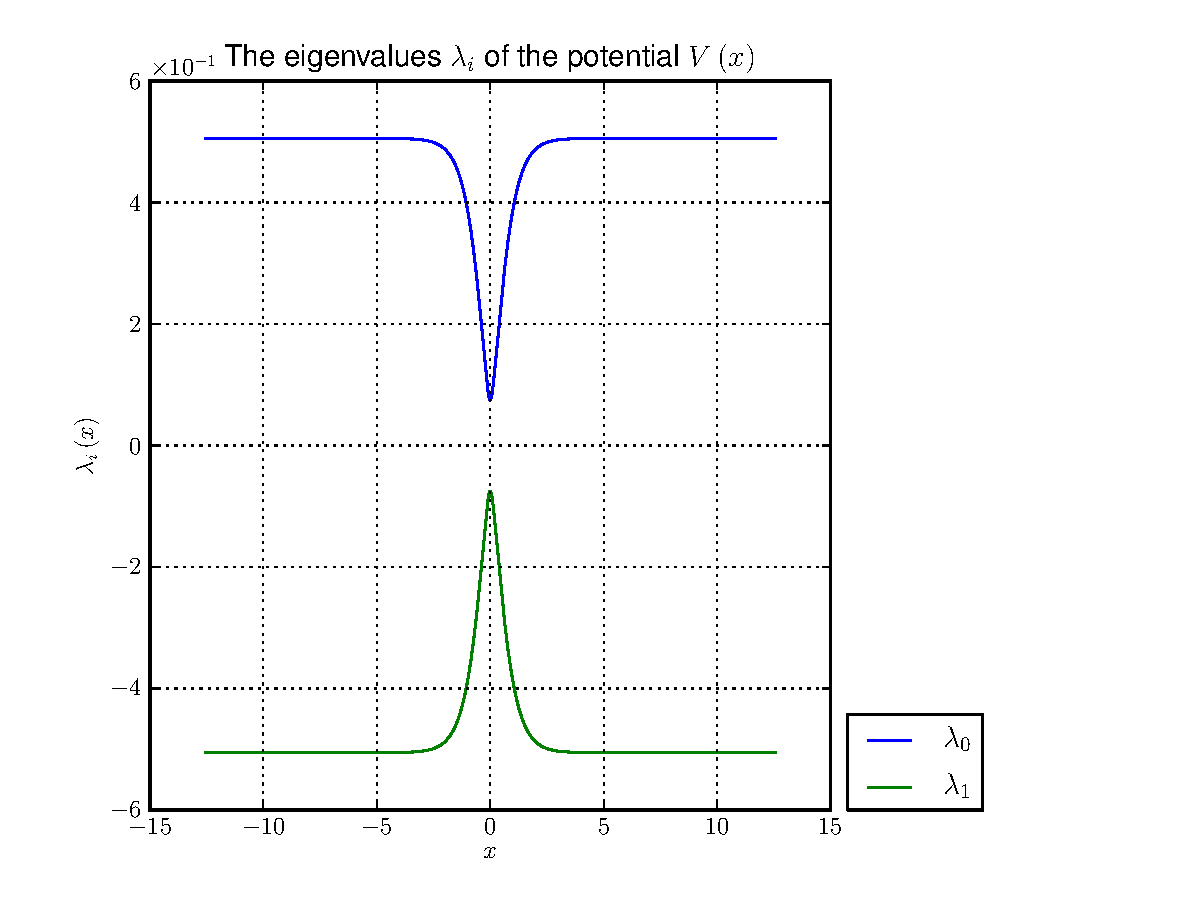
\includegraphics[width=0.7\linewidth]{./figures/avoided_crossing.pdf}
  \caption{A simple potential with two energy levels and a single avoided crossing.}
  \label{fig:avoided_crossing}
\end{figure}


\begin{figure}
  \centering
  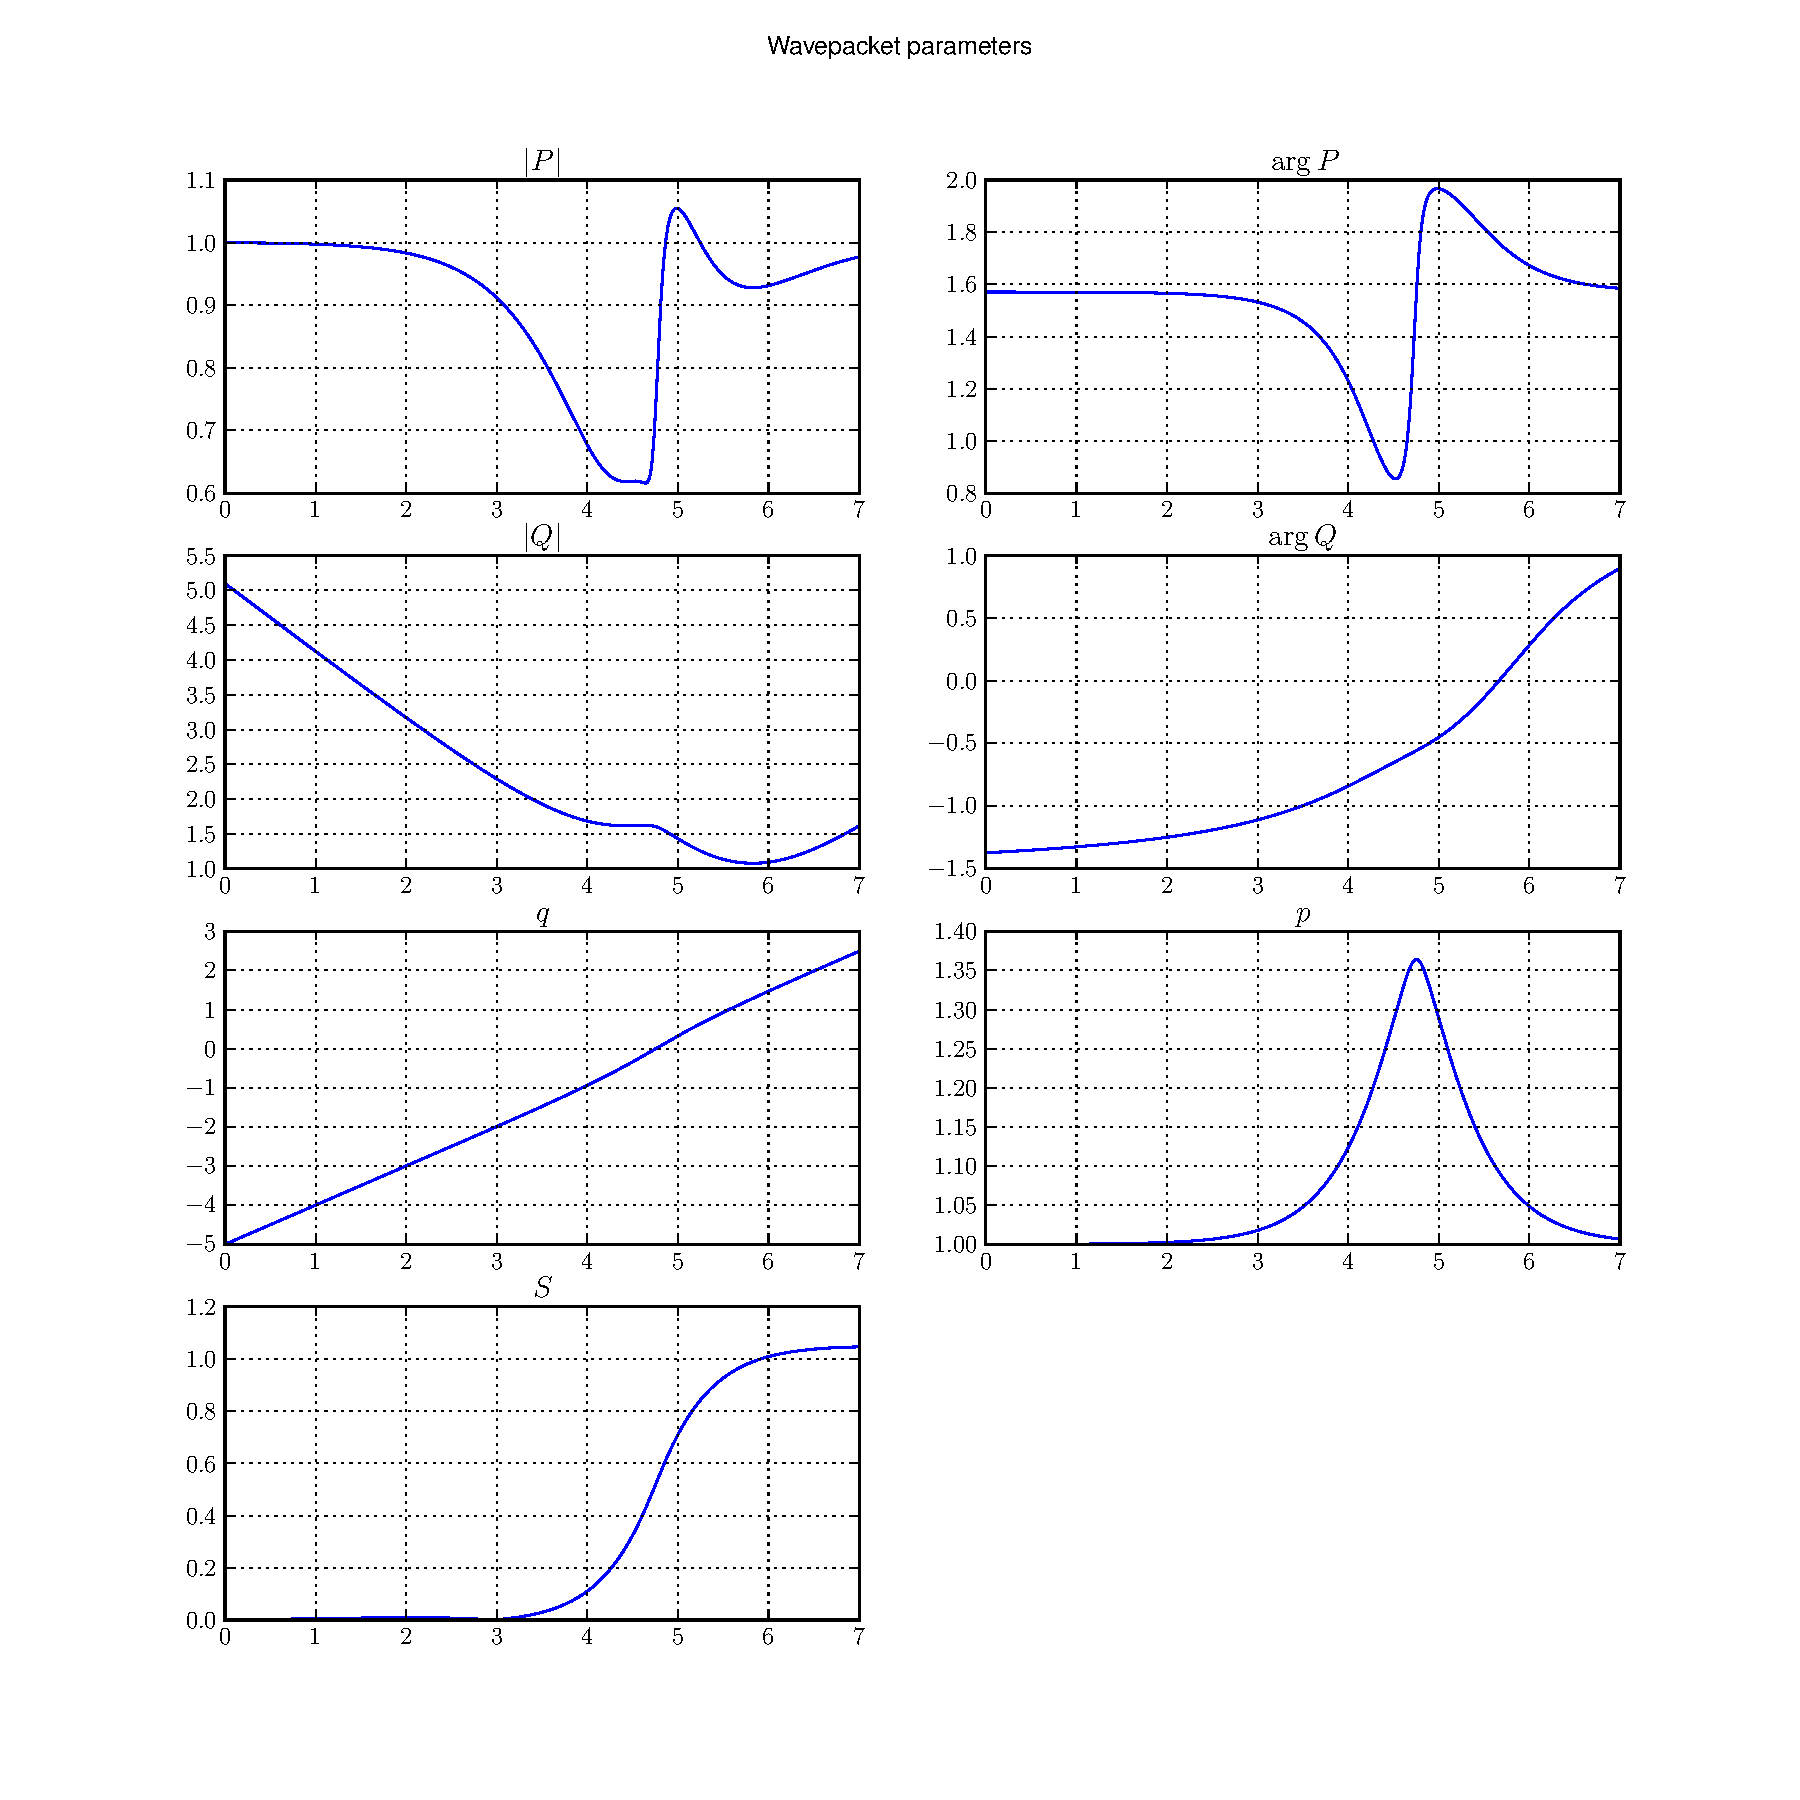
\includegraphics[width=\the\linewidth]{./figures/delta_gap_phi0/wavepacket_parameters_abs_ang_block0.pdf}
  \caption{The parameter set $\Pi$, it is identical to all simulations presented in this section.}
  \label{fig:basic_delta_gap_parameters}
\end{figure}


\begin{figure}[h!]
  \centering
  \subfloat[][]{
    \label{fig:basic_delta_gap_phi0_norm}
    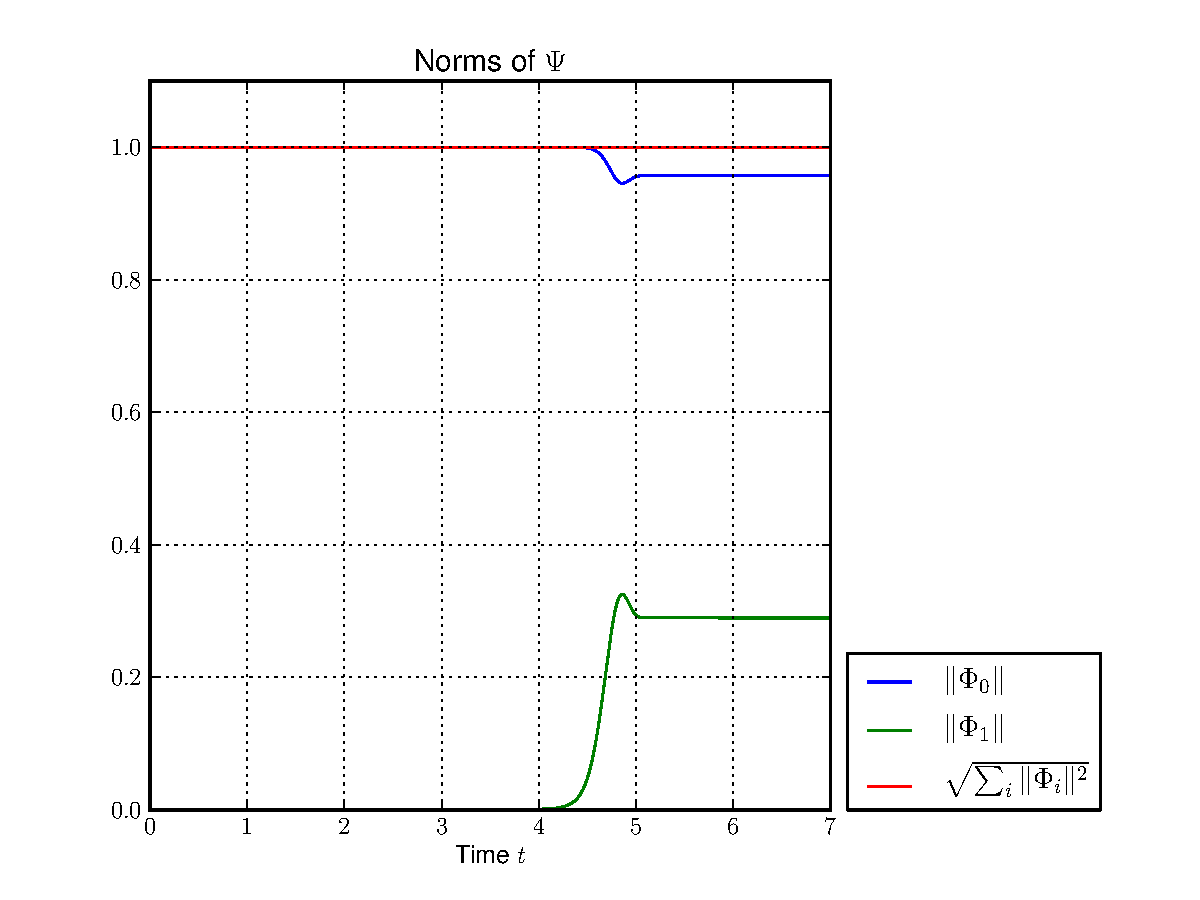
\includegraphics[width=0.5\linewidth]{./figures/delta_gap_phi0/norms_block0.pdf}
  }
  \subfloat[][]{
    \label{fig:basic_delta_gap_phi0_norms_drift}
    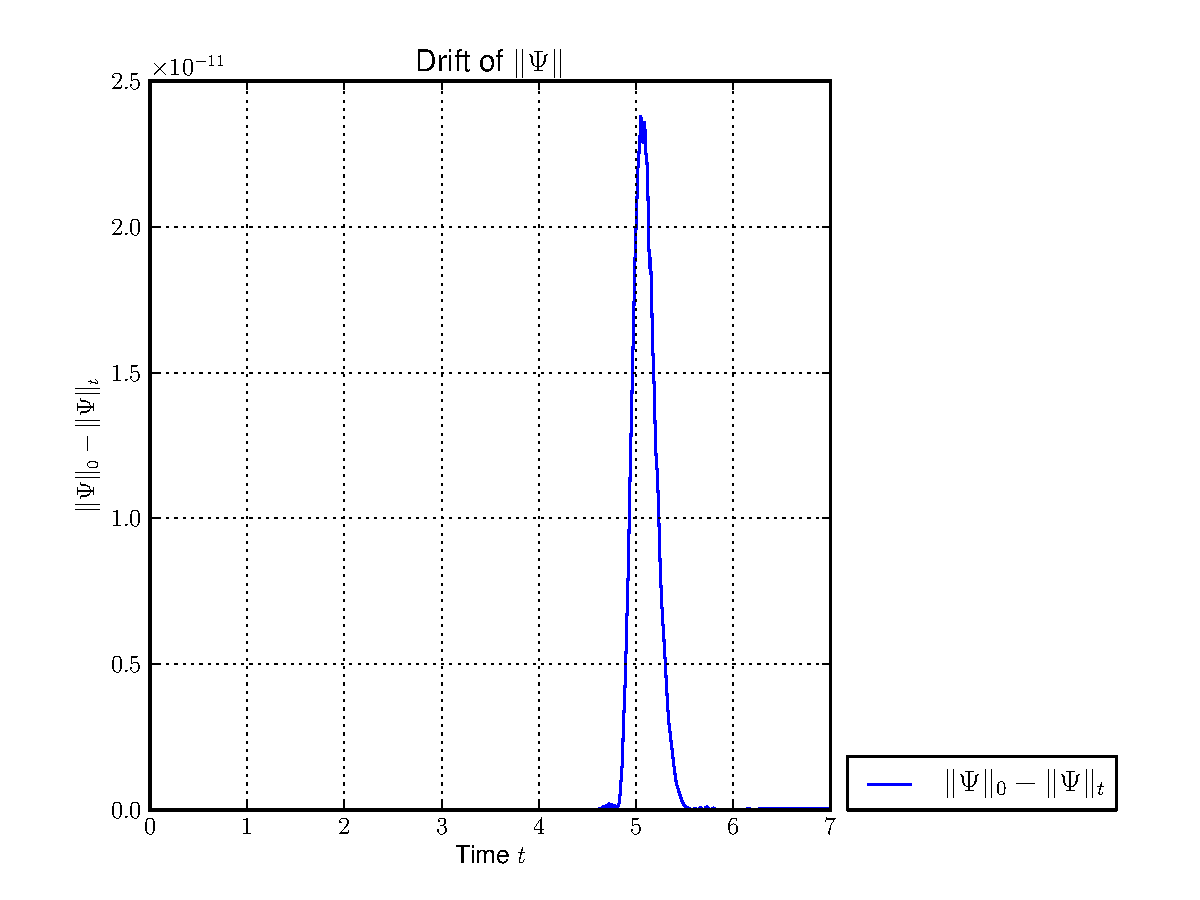
\includegraphics[width=0.5\linewidth]{./figures/delta_gap_phi0/norms_drift_block0.pdf}
  } \\
  \caption[Norms and norm drift for a $\phi_0$ in an avoided crossing]{
  This figure shows the norm of both components $\Phi_0$ and $\Phi_1$ of the
  wavepacket $\Psi$ as well as the overall norm. The right panel shows the drift
  of the overall norm, which should be conserved as good as possible.
  The initial wavepacket $\Ket{\Psi\ofs{t=0}} = \phi_0$ starts on the upper level.
  The full set of simulation parameters is printed in \ref{cfg:delta_gap_phi0}
  \label{fig:basic_delta_gap_phi0_norms}
  }
\end{figure}


\begin{figure}[h!]
  \centering
  \subfloat[][]{
    \label{fig:basic_delta_gap_phi0_energy}
    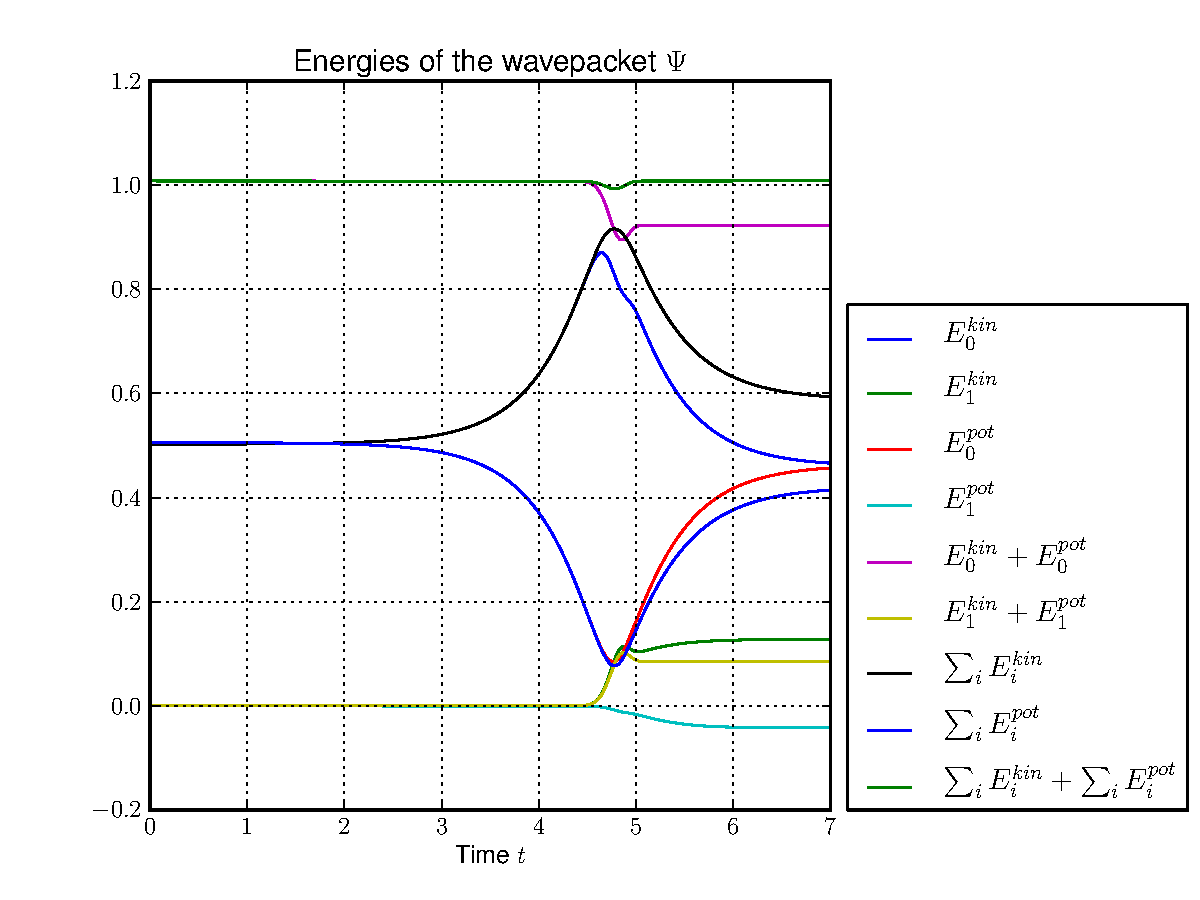
\includegraphics[width=0.5\linewidth]{./figures/delta_gap_phi0/energies_block0.pdf}
  }
  \subfloat[][]{
    \label{fig:basic_delta_gap_phi0_energy_drift}
    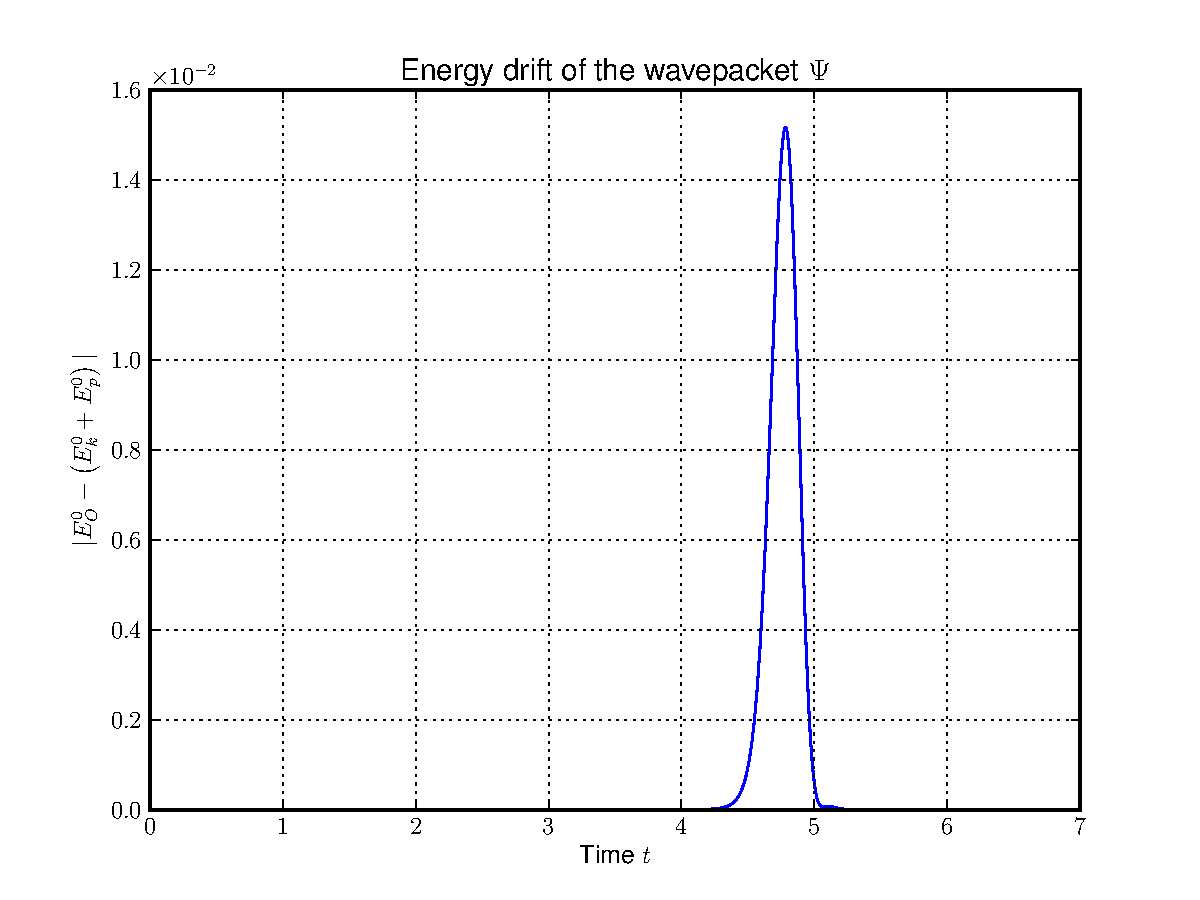
\includegraphics[width=0.5\linewidth]{./figures/delta_gap_phi0/energy_drift_block0.pdf}
  } \\
  \caption[Energies for a $\phi_0$ in an avoided crossing]{
  Kinetic and potential energies and the violation of energy conservation for an
  initial wavepacket $\phi_0$ starting on the upper level. The full set of simulation
  parameters is printed in \ref{cfg:delta_gap_phi0}
  \label{fig:basic_delta_gap_phi0_energies}
  }
\end{figure}



\begin{figure}[h!]
  \centering
  \subfloat[][]{
    \label{fig:basic_delta_gap_phi1_norm}
    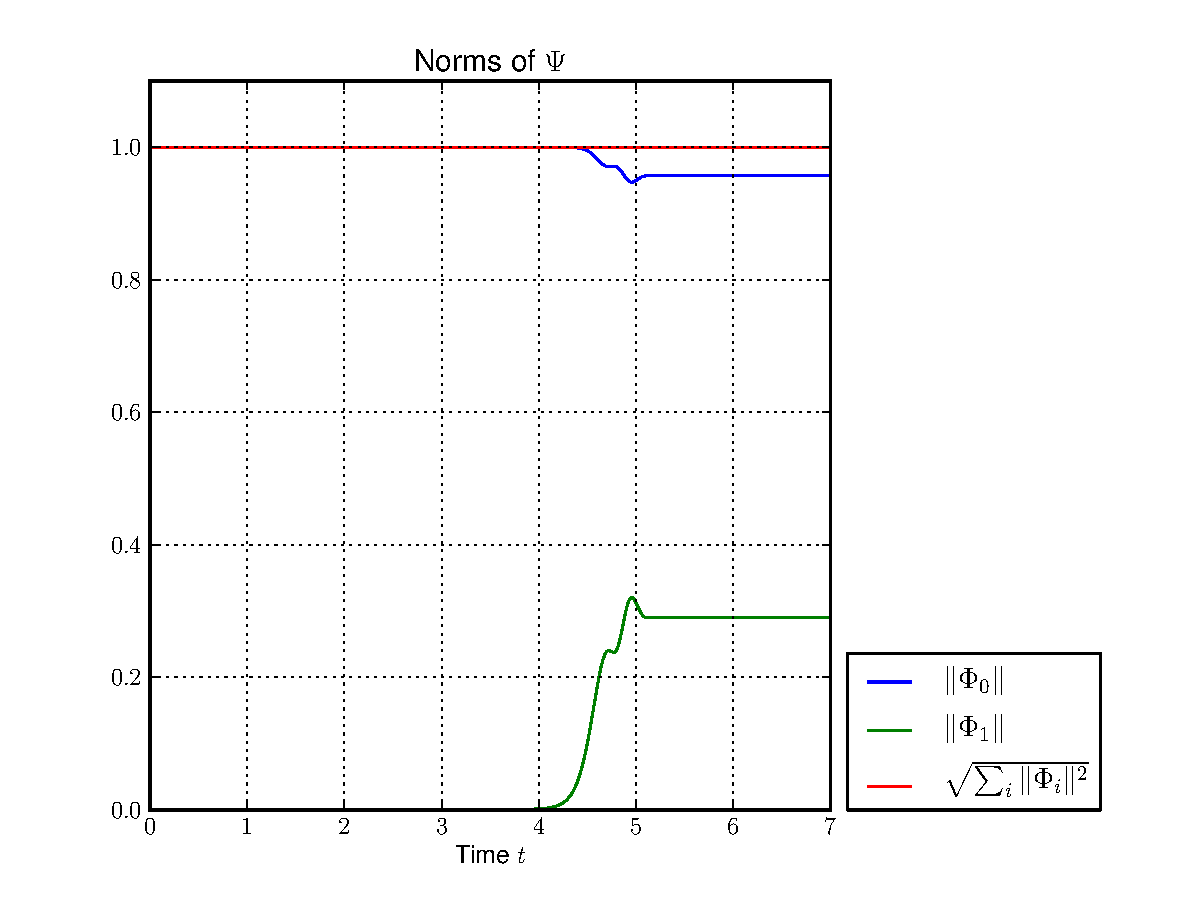
\includegraphics[width=0.5\linewidth]{./figures/delta_gap_phi1/norms_block0.pdf}
  }
  \subfloat[][]{
    \label{fig:basic_delta_gap_phi1_norms_drift}
    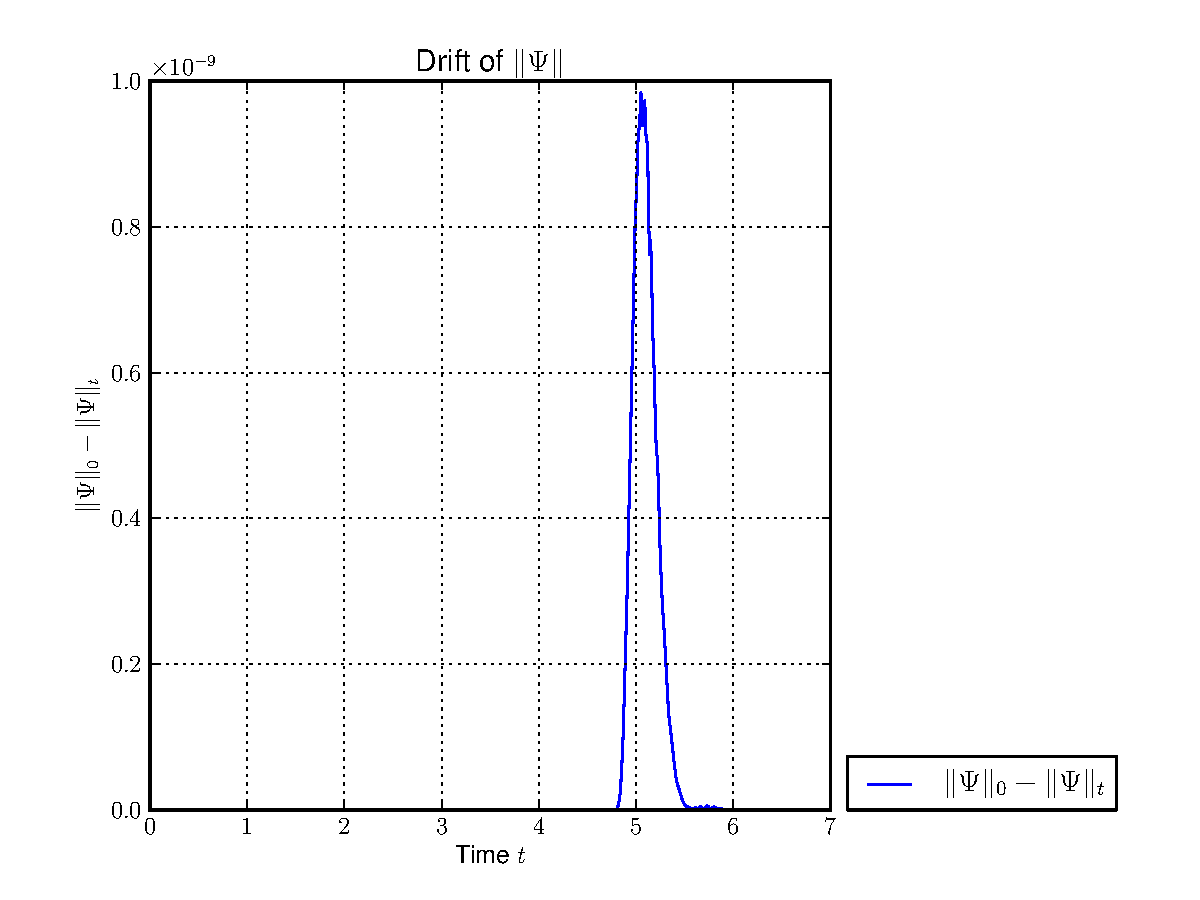
\includegraphics[width=0.5\linewidth]{./figures/delta_gap_phi1/norms_drift_block0.pdf}
  } \\
  \caption[Norms and norm drift for a $\phi_1$ in an avoided crossing]{
  This figure shows the norm of both components $\Phi_0$ and $\Phi_1$ of the
  wavepacket $\Psi$ as well as the overall norm. The right panel shows the drift
  of the overall norm, which should be conserved as good as possible.
  The initial wavepacket $\Ket{\Psi\ofs{t=0}} = \phi_1$ starts on the upper level.
  The full set of simulation parameters is printed in \ref{cfg:delta_gap_phi1}
  \label{fig:basic_delta_gap_phi1_norms}
  }
\end{figure}


\begin{figure}[h!]
  \centering
  \subfloat[][]{
    \label{fig:basic_delta_gap_phi1_energy}
    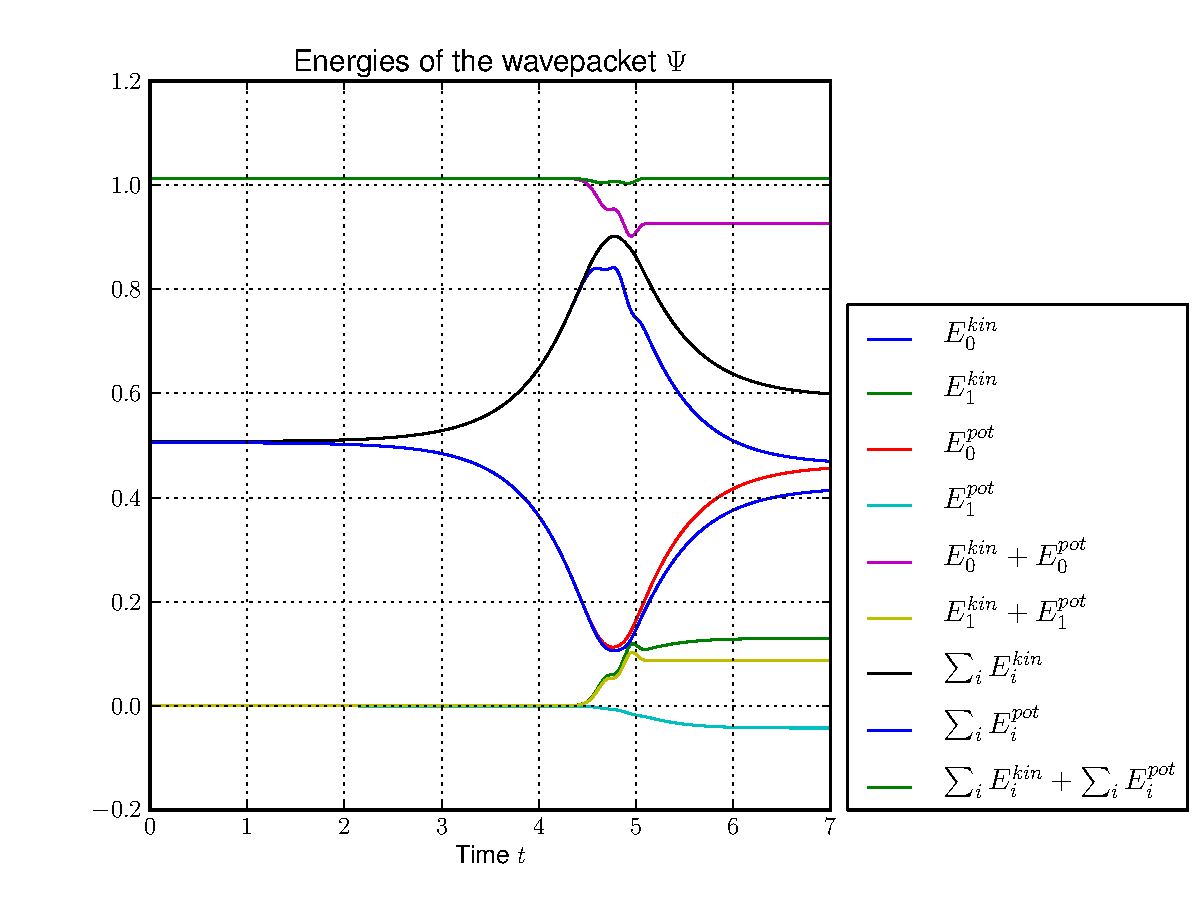
\includegraphics[width=0.5\linewidth]{./figures/delta_gap_phi1/energies_block0.pdf}
  }
  \subfloat[][]{
    \label{fig:basic_delta_gap_phi1_energy_drift}
    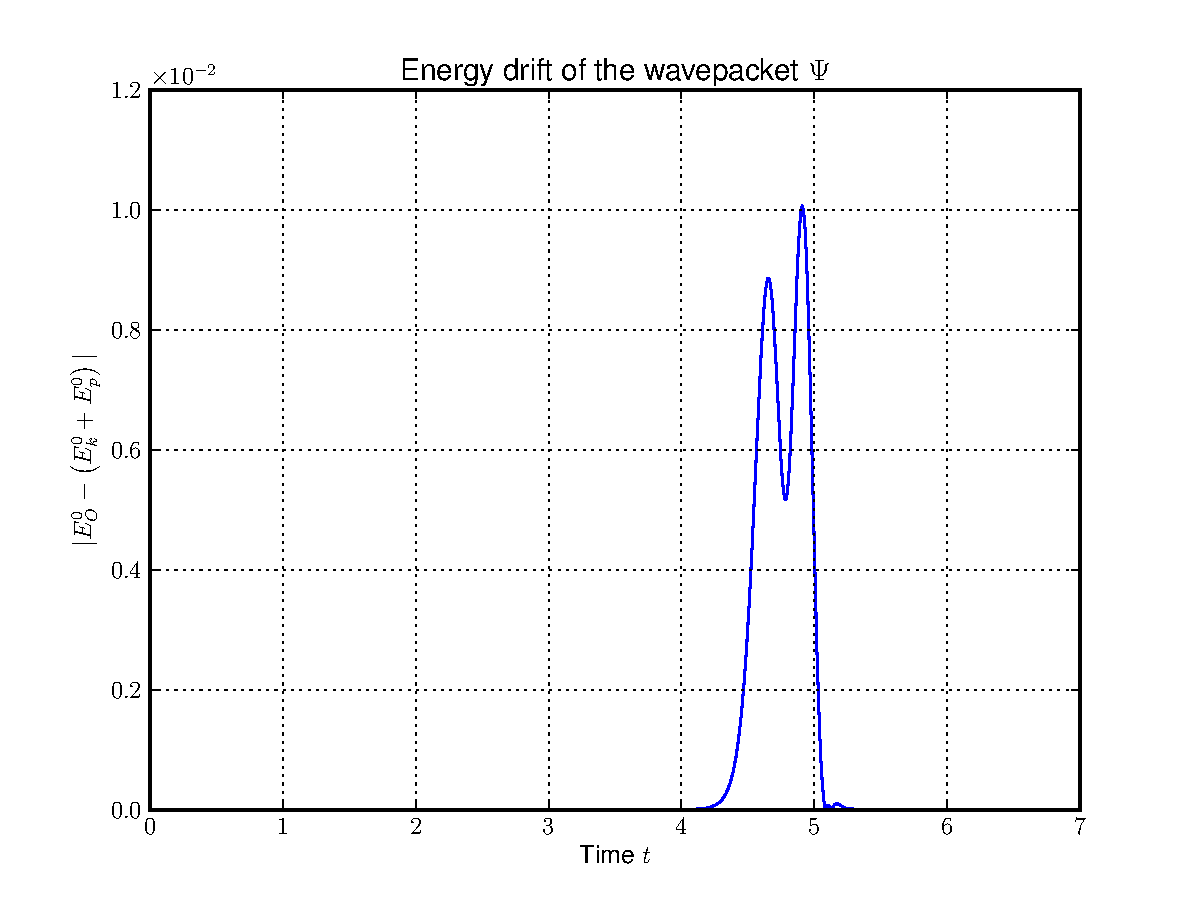
\includegraphics[width=0.5\linewidth]{./figures/delta_gap_phi1/energy_drift_block0.pdf}
  } \\
  \caption[Energies for a $\phi_1$ in an avoided crossing]{
  Kinetic and potential energies and the violation of energy conservation for an
  initial wavepacket $\phi_1$ starting on the upper level. The full set of simulation
  parameters is printed in \ref{cfg:delta_gap_phi1}
  \label{fig:basic_delta_gap_phi1_energies}
  }
\end{figure}



\begin{figure}[h!]
  \centering
  \subfloat[][]{
    \label{fig:basic_delta_gap_phi2_norm}
    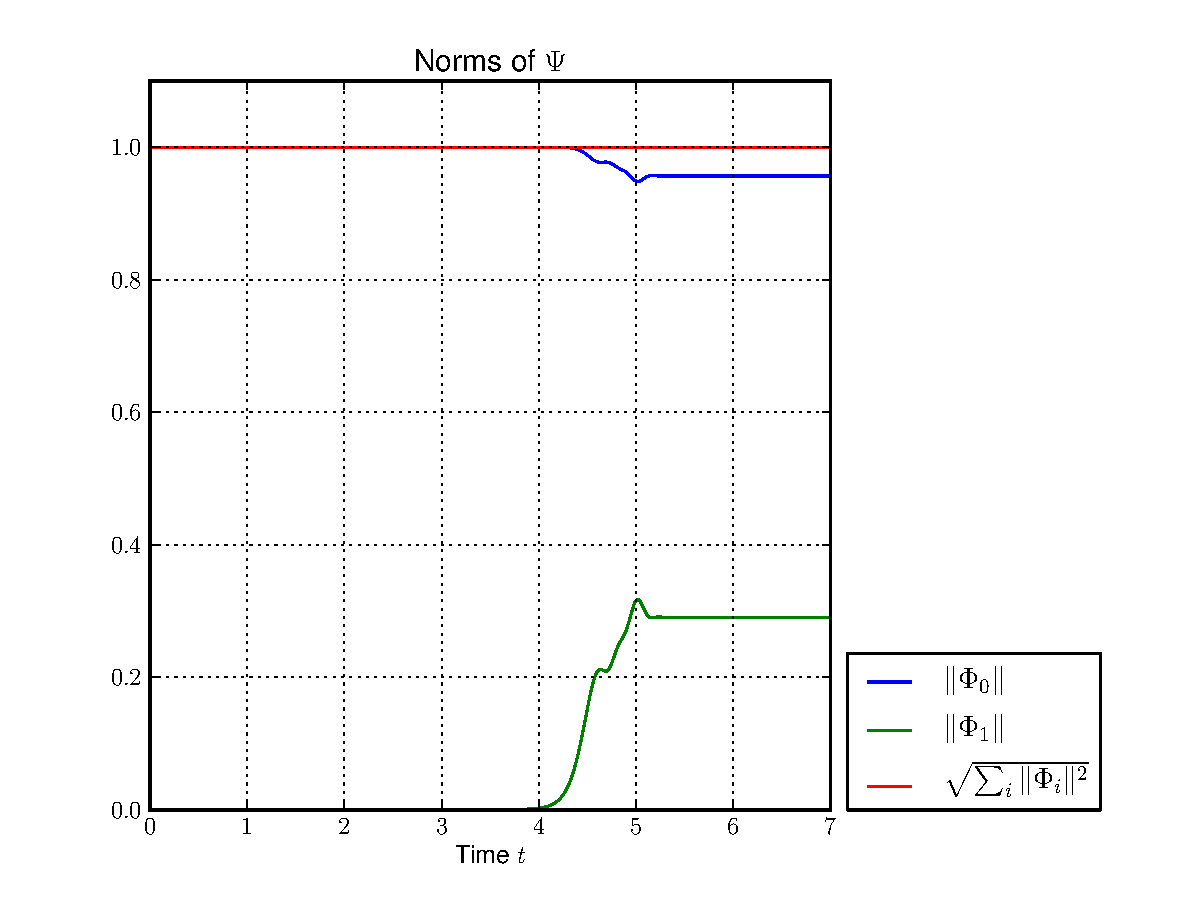
\includegraphics[width=0.5\linewidth]{./figures/delta_gap_phi2/norms_block0.pdf}
  }
  \subfloat[][]{
    \label{fig:basic_delta_gap_phi2_norms_drift}
    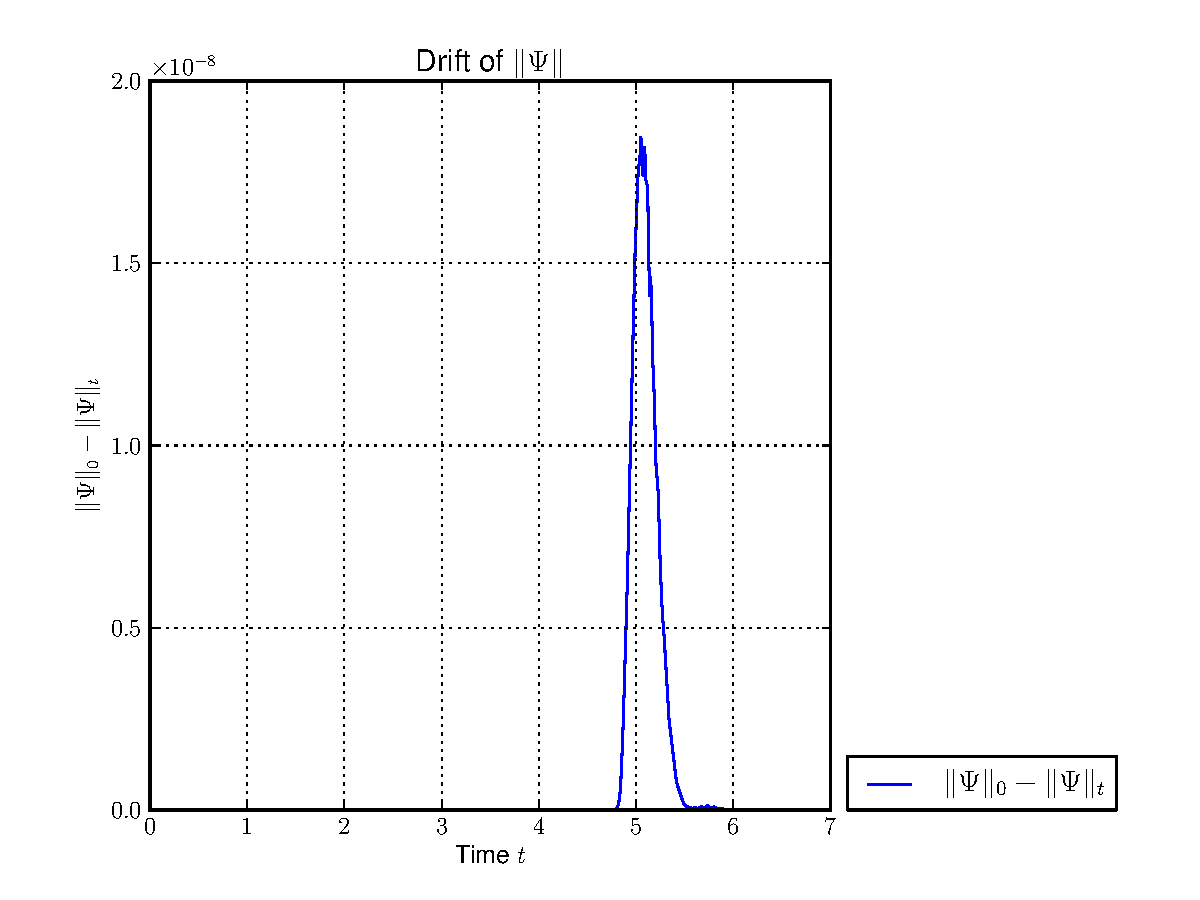
\includegraphics[width=0.5\linewidth]{./figures/delta_gap_phi2/norms_drift_block0.pdf}
  } \\
  \caption[Norms and norm drift for a $\phi_2$ in an avoided crossing]{
  This figure shows the norm of both components $\Phi_0$ and $\Phi_1$ of the
  wavepacket $\Psi$ as well as the overall norm. The right panel shows the drift
  of the overall norm, which should be conserved as good as possible.
  The initial wavepacket $\Ket{\Psi\ofs{t=0}} = \phi_2$ starts on the upper level.
  The full set of simulation parameters is printed in \ref{cfg:delta_gap_phi2}
  \label{fig:basic_delta_gap_phi2_norms}
  }
\end{figure}


\begin{figure}[h!]
  \centering
  \subfloat[][]{
    \label{fig:basic_delta_gap_phi2_energy}
    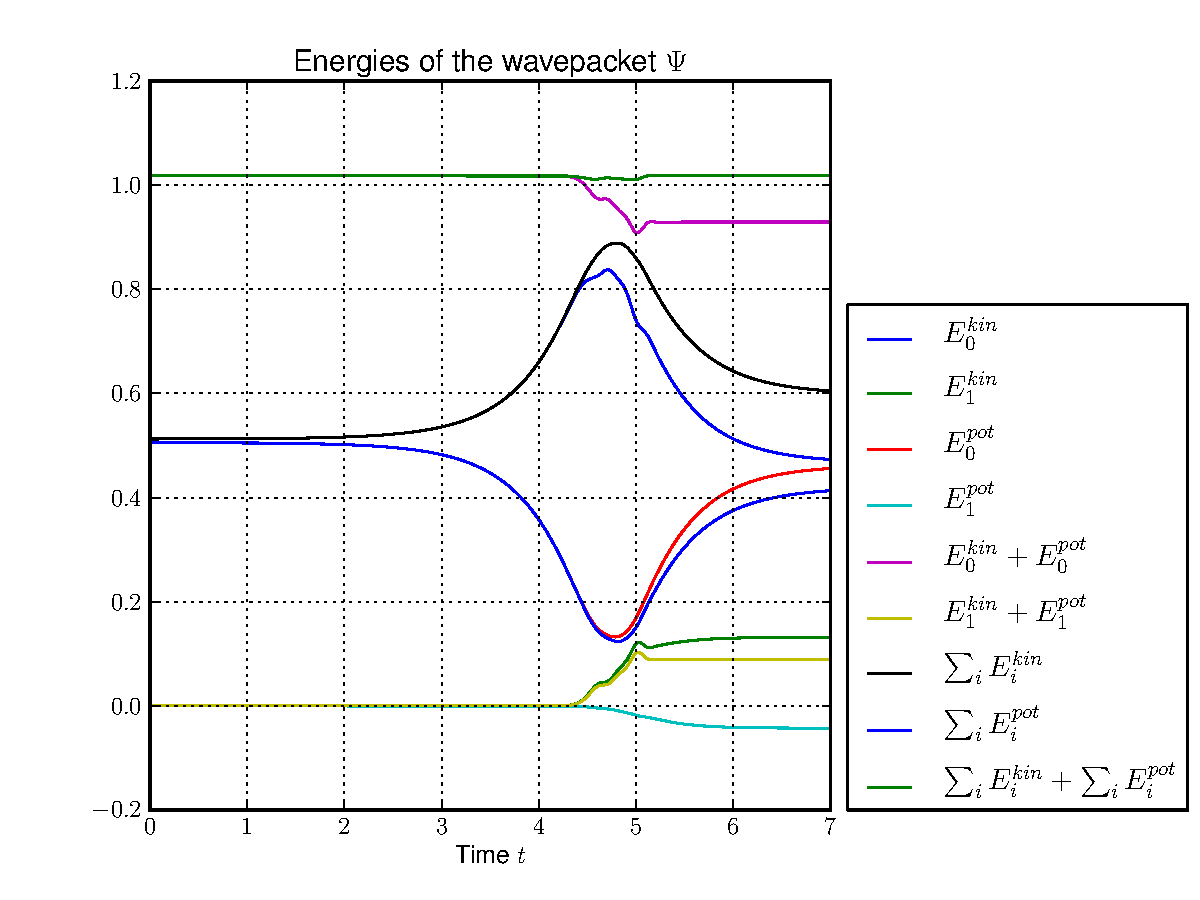
\includegraphics[width=0.5\linewidth]{./figures/delta_gap_phi2/energies_block0.pdf}
  }
  \subfloat[][]{
    \label{fig:basic_delta_gap_phi2_energy_drift}
    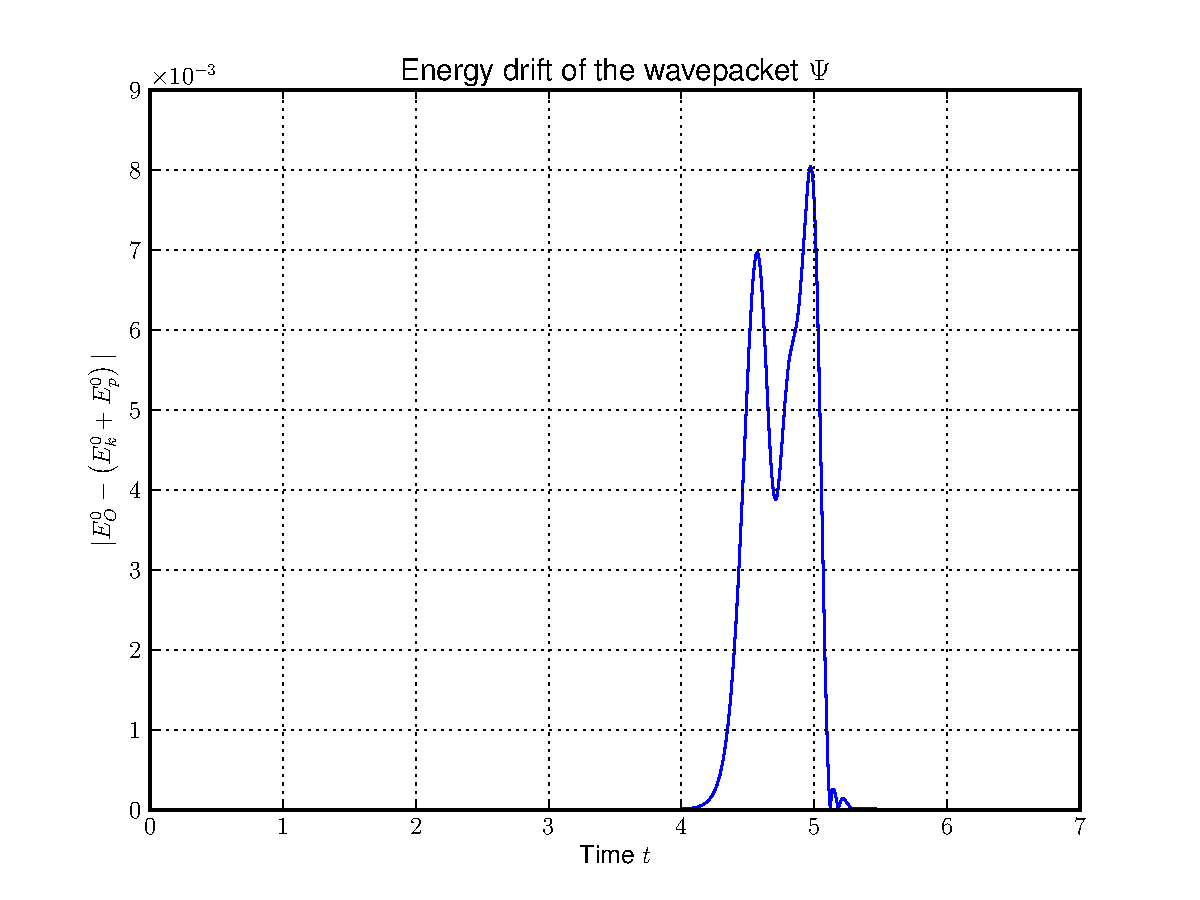
\includegraphics[width=0.5\linewidth]{./figures/delta_gap_phi2/energy_drift_block0.pdf}
  } \\
  \caption[Energies for a $\phi_2$ in an avoided crossing]{
  Kinetic and potential energies and the violation of energy conservation for an
  initial wavepacket $\phi_2$ starting on the upper level. The full set of simulation
  parameters is printed in \ref{cfg:delta_gap_phi2}
  \label{fig:basic_delta_gap_phi2_energies}
  }
\end{figure}



\begin{figure}[h!]
  \centering
  \subfloat[][]{
    \label{fig:basic_delta_gap_phi3_norm}
    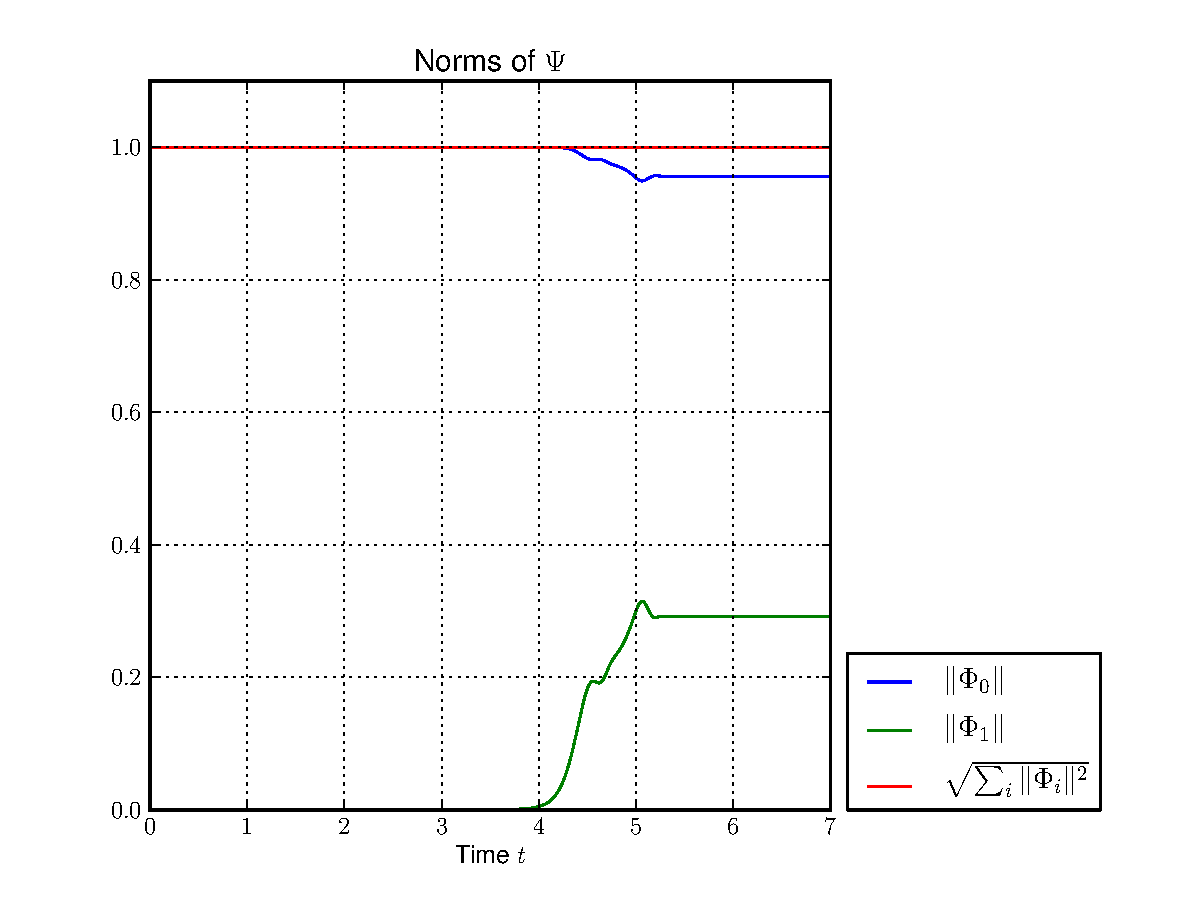
\includegraphics[width=0.5\linewidth]{./figures/delta_gap_phi3/norms_block0.pdf}
  }
  \subfloat[][]{
    \label{fig:basic_delta_gap_phi3_norms_drift}
    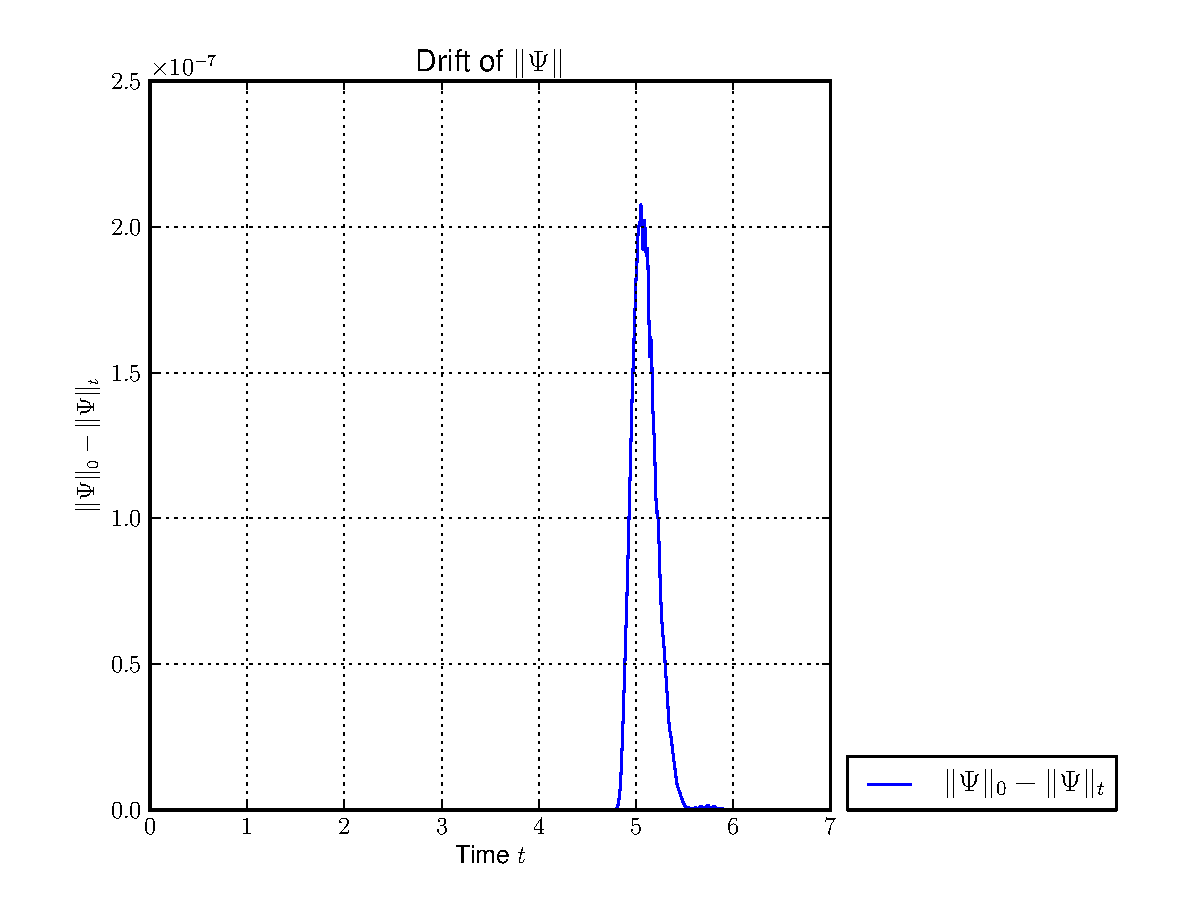
\includegraphics[width=0.5\linewidth]{./figures/delta_gap_phi3/norms_drift_block0.pdf}
  } \\
  \caption[Norms and norm drift for a $\phi_3$ in an avoided crossing]{
  This figure shows the norm of both components $\Phi_0$ and $\Phi_1$ of the
  wavepacket $\Psi$ as well as the overall norm. The right panel shows the drift
  of the overall norm, which should be conserved as good as possible.
  The initial wavepacket $\Ket{\Psi\ofs{t=0}} = \phi_3$ starts on the upper level.
  The full set of simulation parameters is printed in \ref{cfg:delta_gap_phi3}
  \label{fig:basic_delta_gap_phi3_norms}
  }
\end{figure}


\begin{figure}[h!]
  \centering
  \subfloat[][]{
    \label{fig:basic_delta_gap_phi3_energy}
    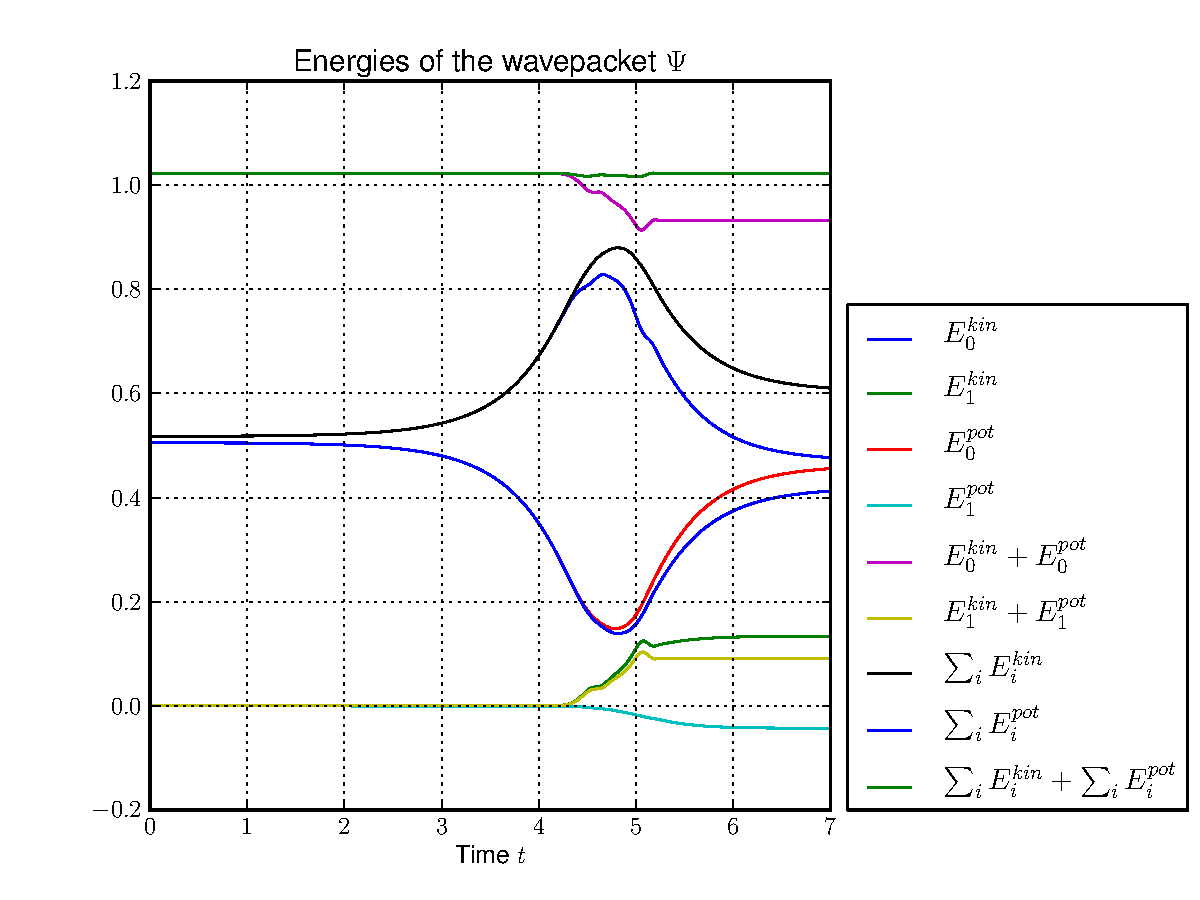
\includegraphics[width=0.5\linewidth]{./figures/delta_gap_phi3/energies_block0.pdf}
  }
  \subfloat[][]{
    \label{fig:basic_delta_gap_phi3_energy_drift}
    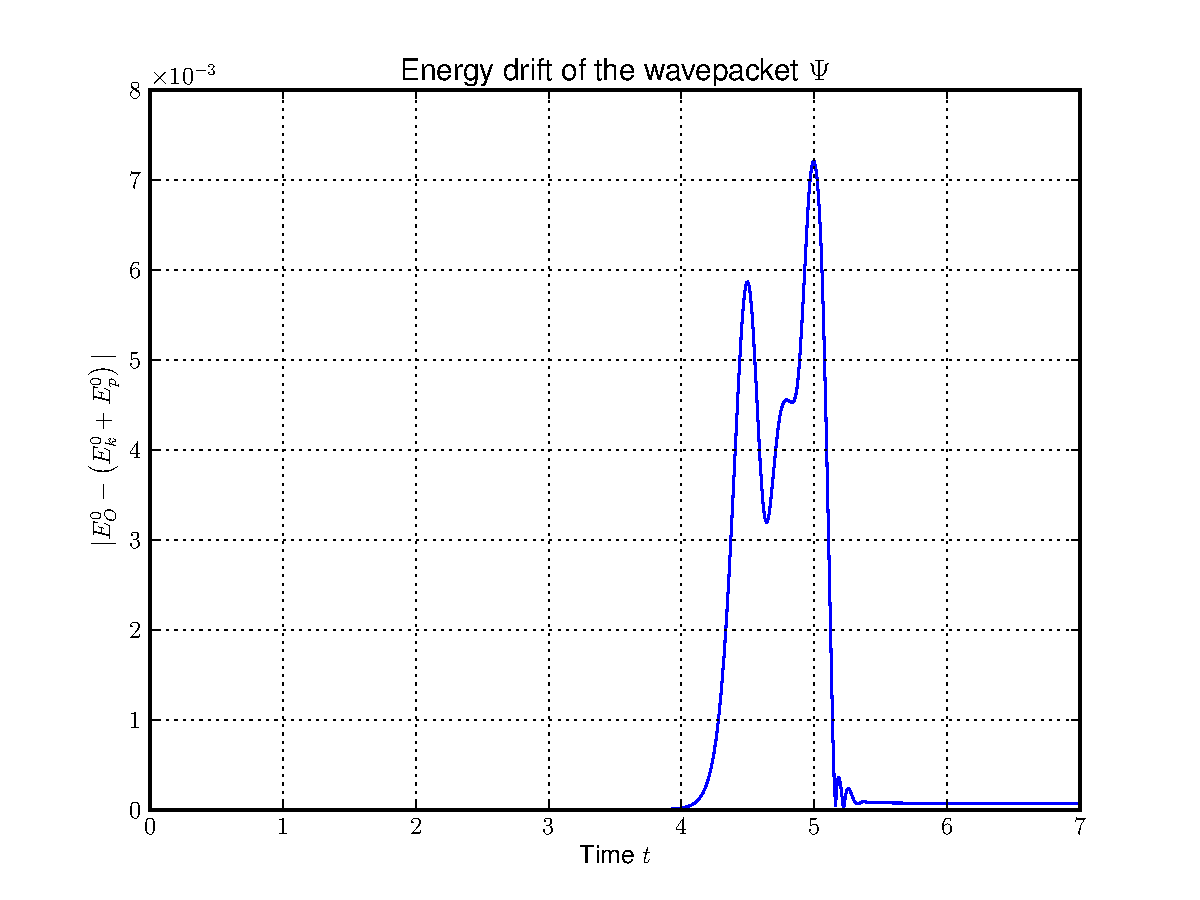
\includegraphics[width=0.5\linewidth]{./figures/delta_gap_phi3/energy_drift_block0.pdf}
  } \\
  \caption[Energies for a $\phi_3$ in an avoided crossing]{
  Kinetic and potential energies and the violation of energy conservation for an
  initial wavepacket $\phi_3$ starting on the upper level. The full set of simulation
  parameters is printed in \ref{cfg:delta_gap_phi3}
  \label{fig:basic_delta_gap_phi3_energies}
  }
\end{figure}



\begin{figure}[h!]
  \centering
  \subfloat[][]{
    \label{fig:basic_delta_gap_phi4_norm}
    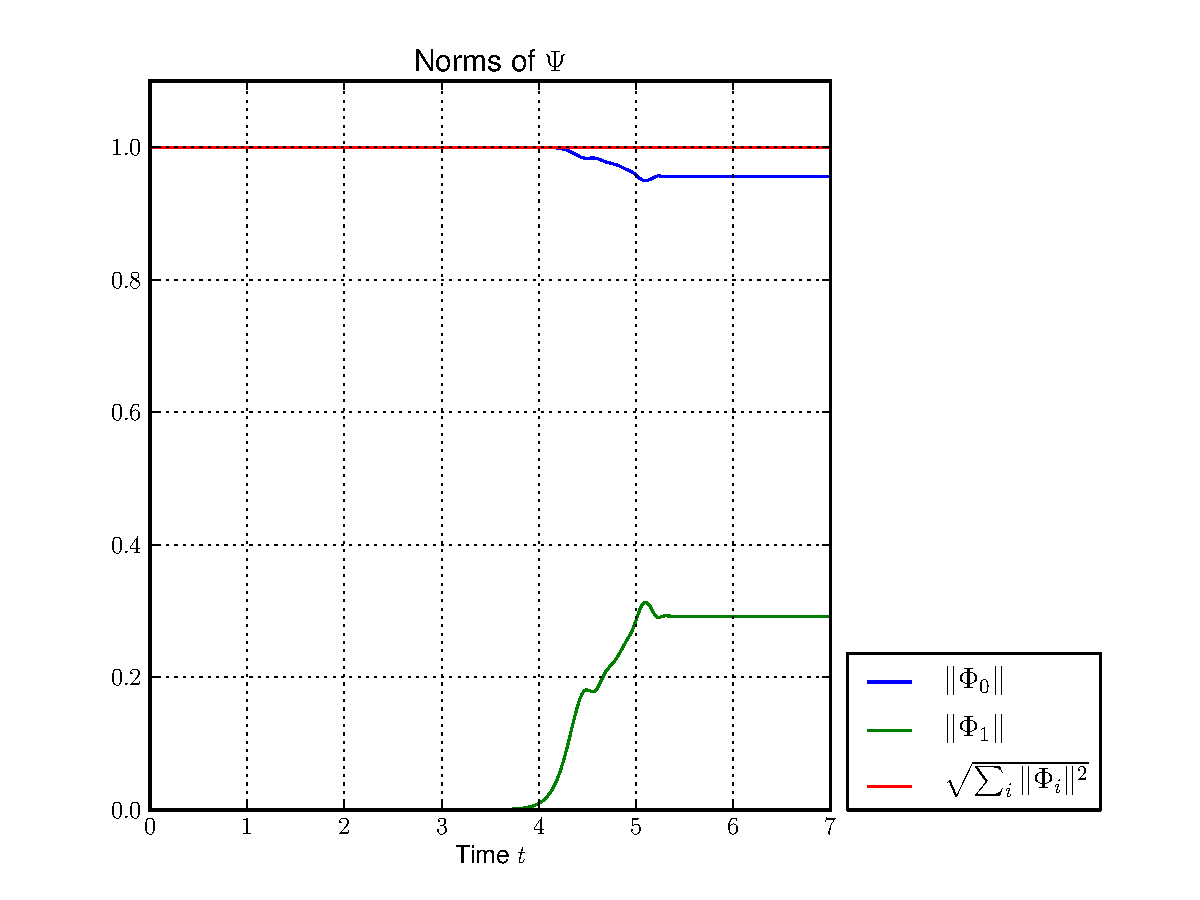
\includegraphics[width=0.5\linewidth]{./figures/delta_gap_phi4/norms_block0.pdf}
  }
  \subfloat[][]{
    \label{fig:basic_delta_gap_phi4_norms_drift}
    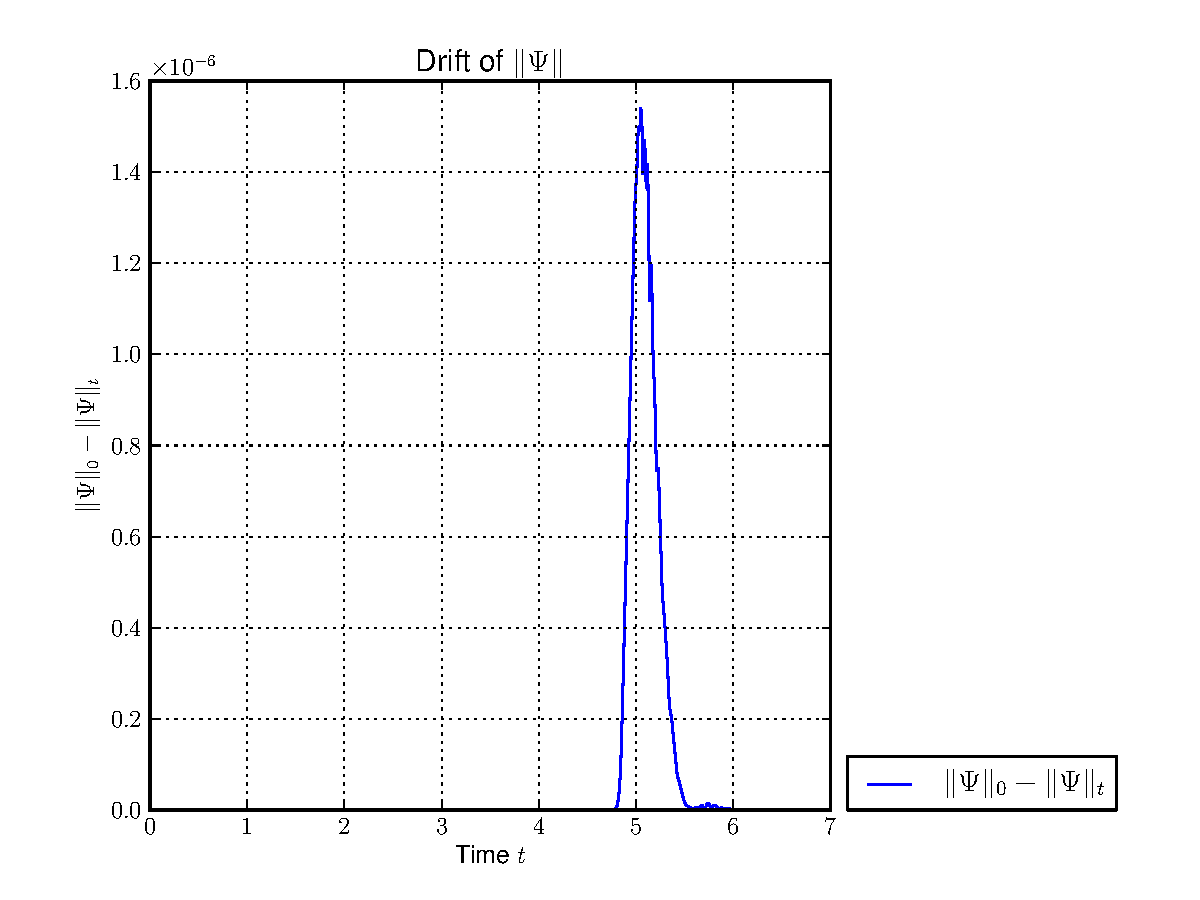
\includegraphics[width=0.5\linewidth]{./figures/delta_gap_phi4/norms_drift_block0.pdf}
  } \\
  \caption[Norms and norm drift for a $\phi_4$ in an avoided crossing]{
  This figure shows the norm of both components $\Phi_0$ and $\Phi_1$ of the
  wavepacket $\Psi$ as well as the overall norm. The right panel shows the drift
  of the overall norm, which should be conserved as good as possible.
  The initial wavepacket $\Ket{\Psi\ofs{t=0}} = \phi_4$ starts on the upper level.
  The full set of simulation parameters is printed in \ref{cfg:delta_gap_phi4}
  \label{fig:basic_delta_gap_phi4_norms}
  }
\end{figure}


\begin{figure}[h!]
  \centering
  \subfloat[][]{
    \label{fig:basic_delta_gap_phi4_energy}
    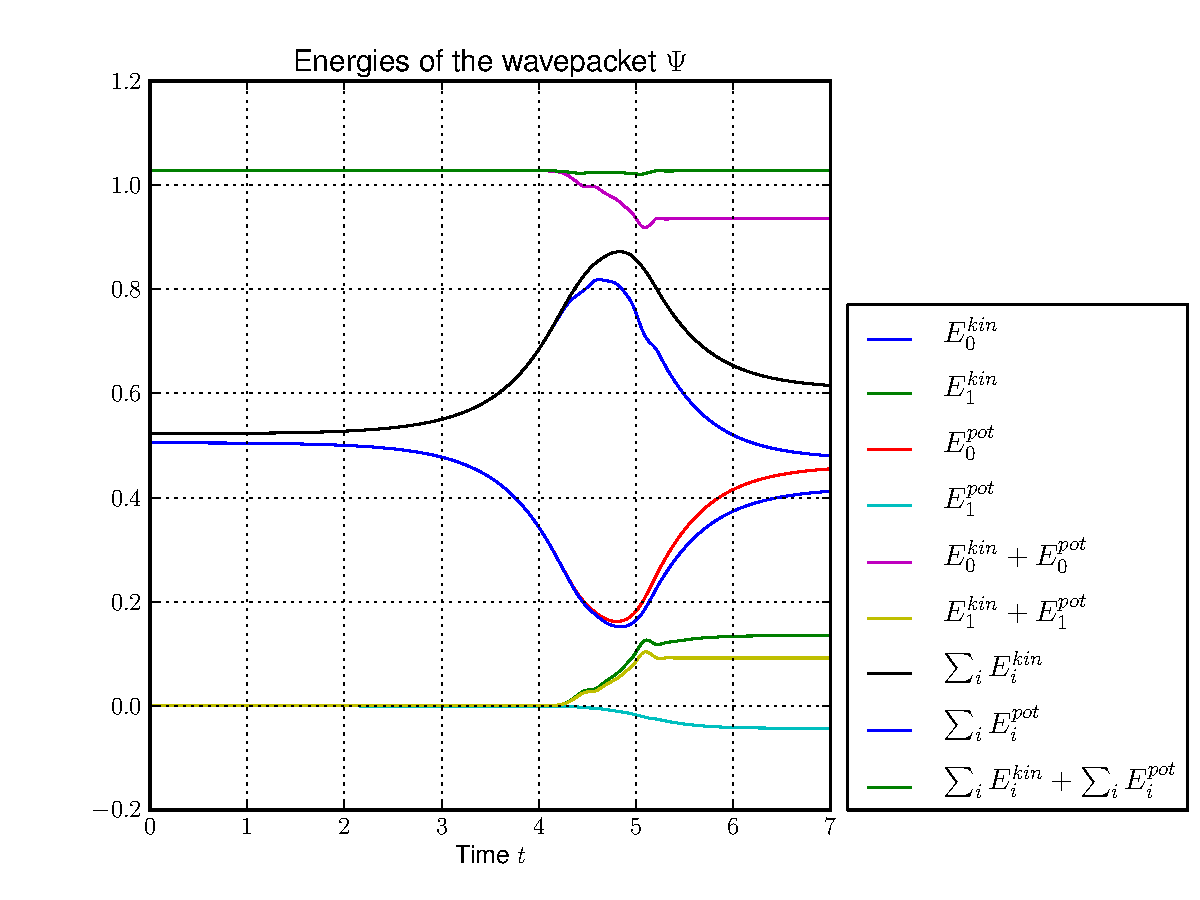
\includegraphics[width=0.5\linewidth]{./figures/delta_gap_phi4/energies_block0.pdf}
  }
  \subfloat[][]{
    \label{fig:basic_delta_gap_phi4_energy_drift}
    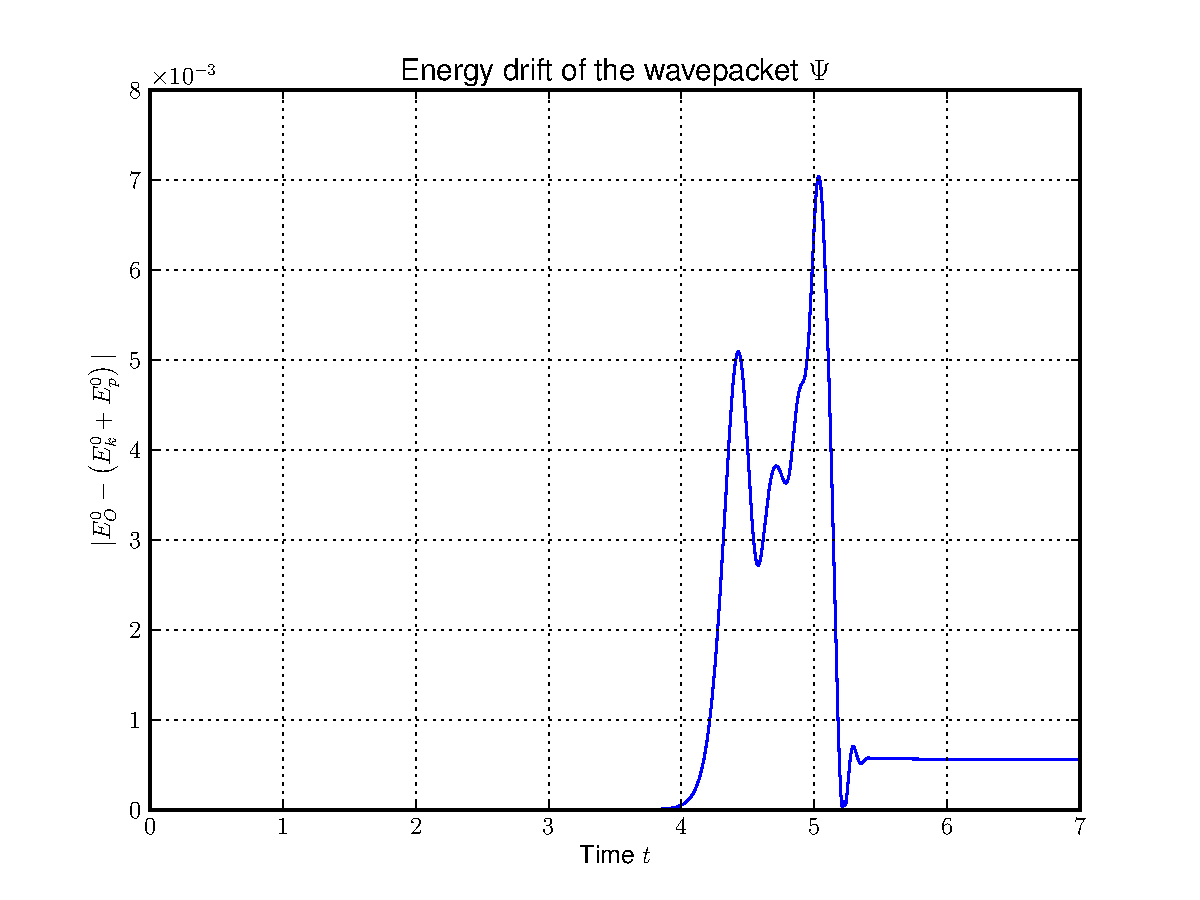
\includegraphics[width=0.5\linewidth]{./figures/delta_gap_phi4/energy_drift_block0.pdf}
  } \\
  \caption[Energies for a $\phi_4$ in an avoided crossing]{
  Kinetic and potential energies and the violation of energy conservation for an
  initial wavepacket $\phi_4$ starting on the upper level. The full set of simulation
  parameters is printed in \ref{cfg:delta_gap_phi4}
  \label{fig:basic_delta_gap_phi4_energies}
  }
\end{figure}



\begin{figure}[h!]
  \centering
  \subfloat[][]{
    \label{fig:basic_delta_gap_phi0phi1_norm}
    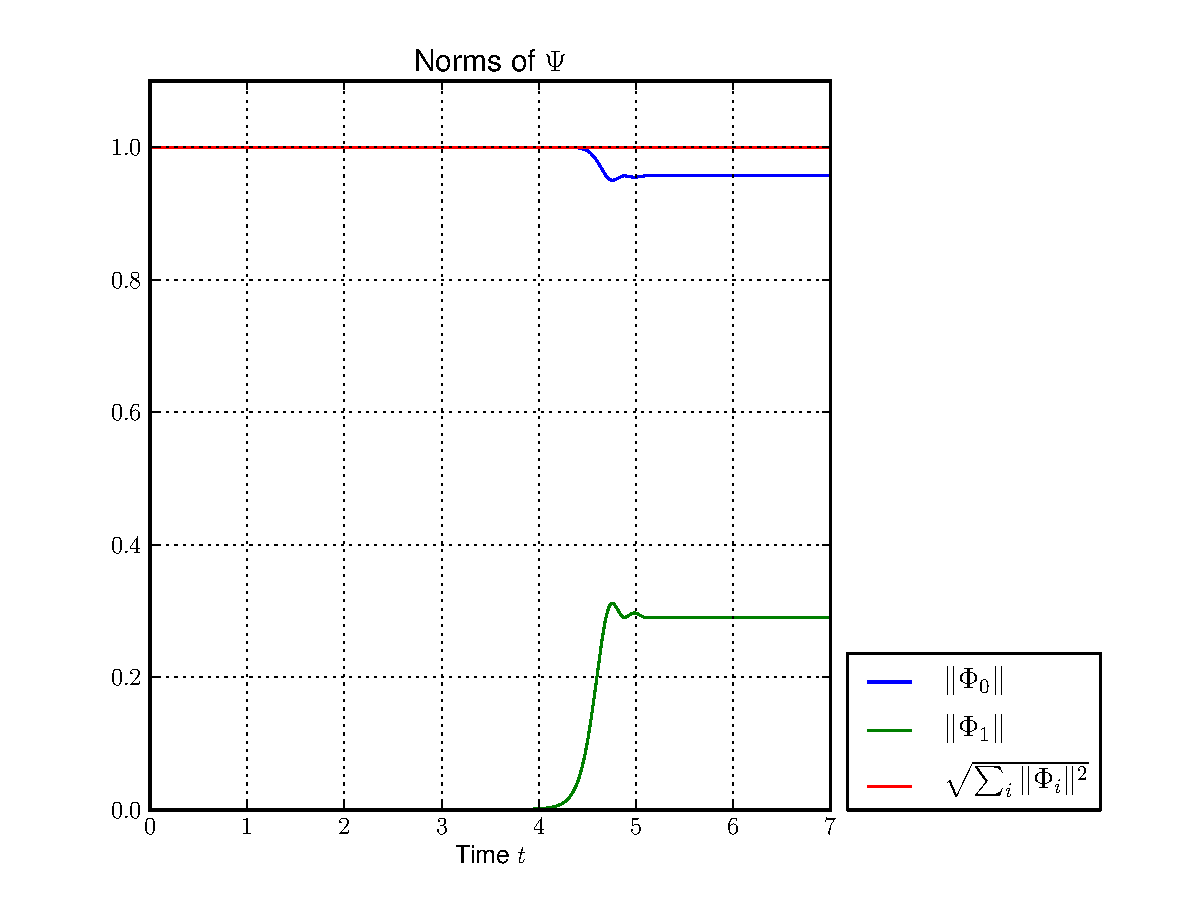
\includegraphics[width=0.5\linewidth]{./figures/delta_gap_phi0phi1/norms_block0.pdf}
  }
  \subfloat[][]{
    \label{fig:basic_delta_gap_phi0phi1_norms_drift}
    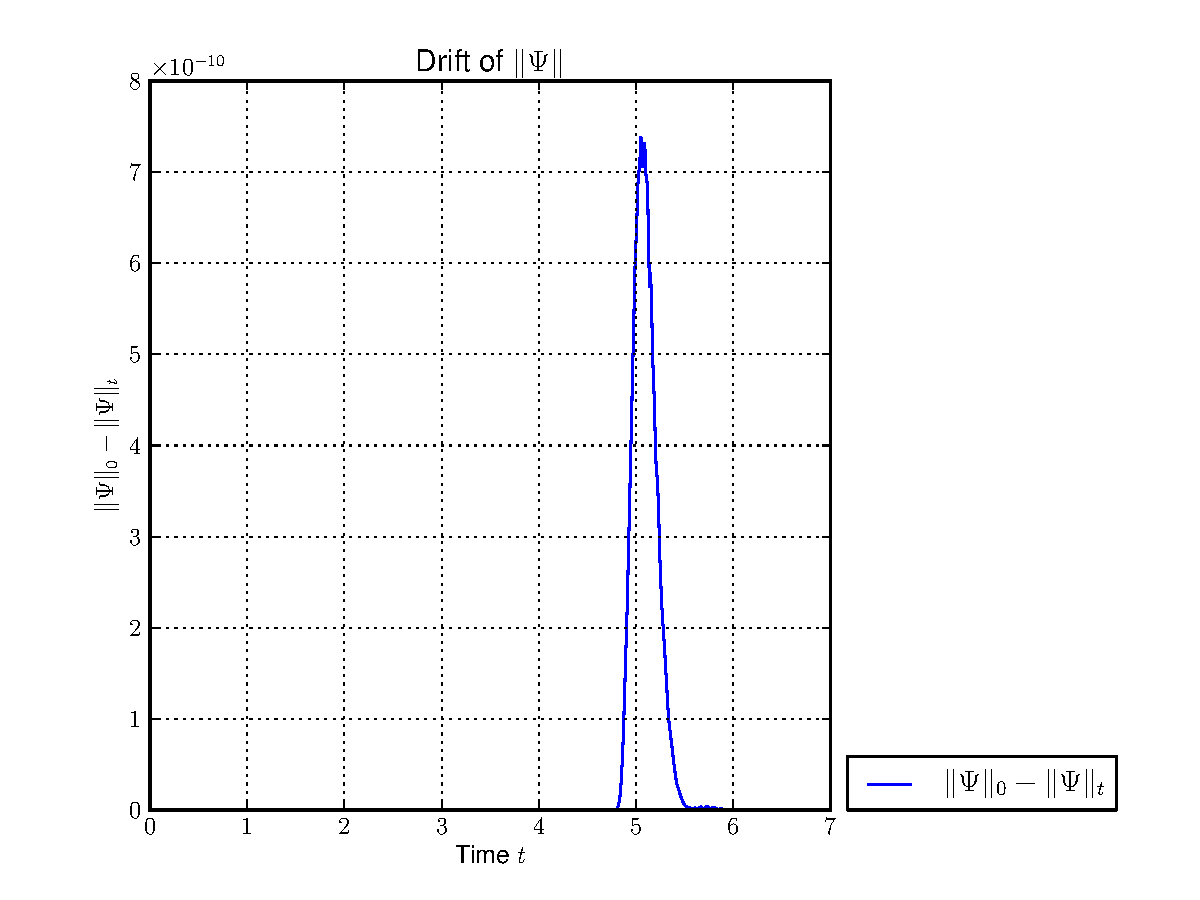
\includegraphics[width=0.5\linewidth]{./figures/delta_gap_phi0phi1/norms_drift_block0.pdf}
  } \\
  \caption[Norms and norm drift for a superposition $\phi_0+\phi_1$ in an avoided crossing]{
  This figure shows the norm of both components $\Phi_0$ and $\Phi_1$ of the
  wavepacket $\Psi$ as well as the overall norm. The right panel shows the drift
  of the overall norm, which should be conserved as good as possible.
  The initial wavepacket $\Ket{\Psi\ofs{t=0}} = \phi_0 + \phi_1$ starts on the
  upper level. The full set of simulation parameters is printed in \ref{cfg:delta_gap_phi0phi1}
  \label{fig:basic_delta_gap_phi0phi1_norms}
  }
\end{figure}


\begin{figure}[h!]
  \centering
  \subfloat[][]{
    \label{fig:basic_delta_gap_phi0phi1_energy}
    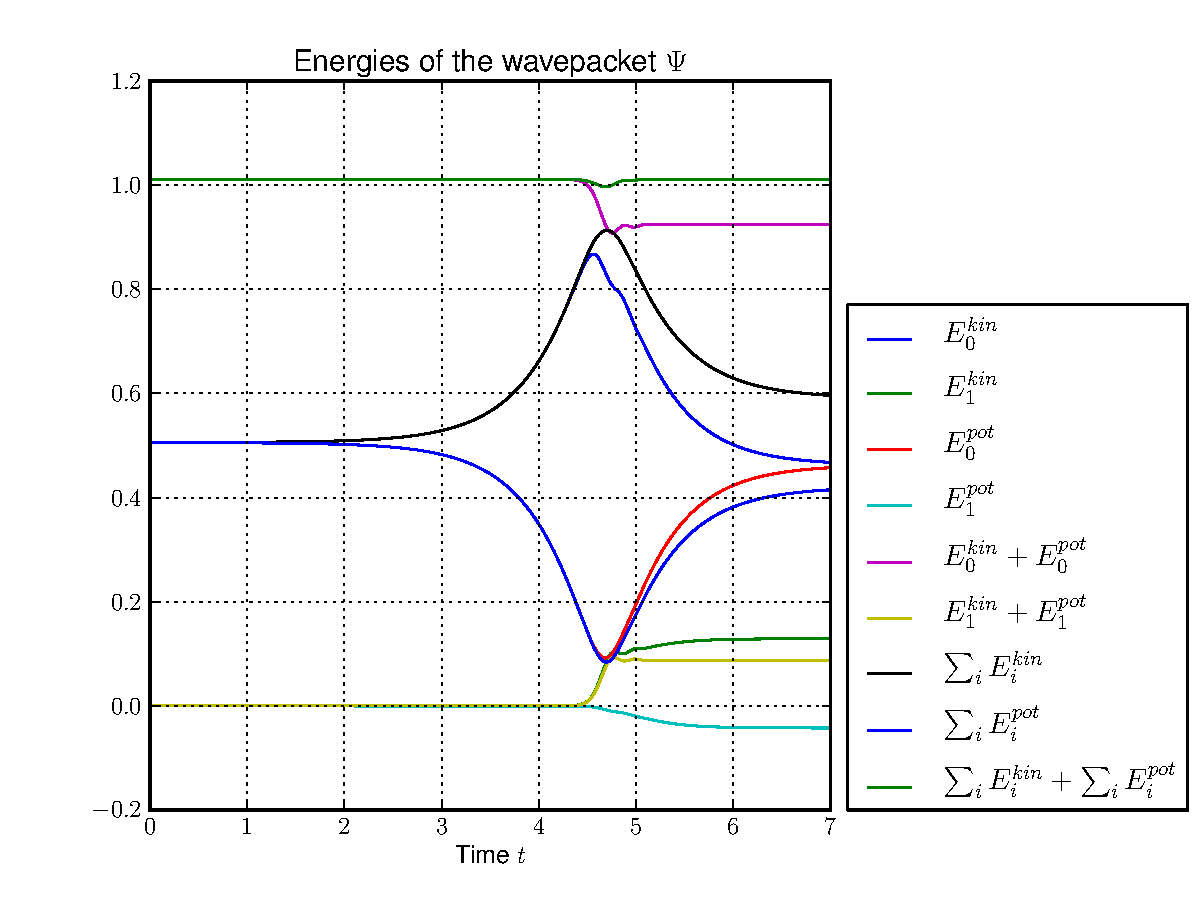
\includegraphics[width=0.5\linewidth]{./figures/delta_gap_phi0phi1/energies_block0.pdf}
  }
  \subfloat[][]{
    \label{fig:basic_delta_gap_phi0phi1_energy_drift}
    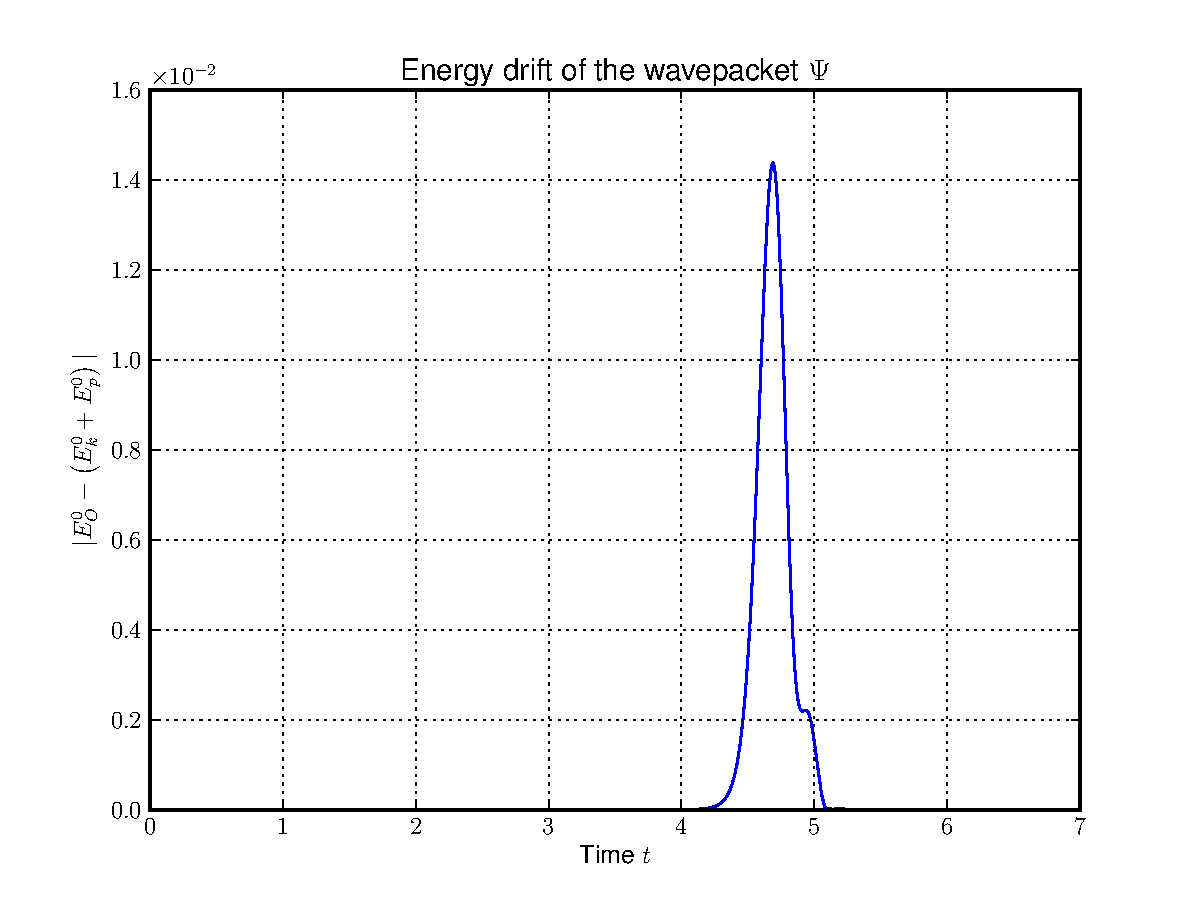
\includegraphics[width=0.5\linewidth]{./figures/delta_gap_phi0phi1/energy_drift_block0.pdf}
  } \\
  \caption[Energies for a superposition of $\phi_0$ and $\phi_1$ in an avoided crossing]{
  Kinetic and potential energies and the violation of energy conservation for an
  initial superposition of $\phi_0$ and $\phi_1$ starting on the upper level. The
  full set of simulation parameters is printed in \ref{cfg:delta_gap_phi0phi1}
  \label{fig:basic_delta_gap_phi0phi1_energies}
  }
\end{figure}



\begin{figure}[h!]
  \centering
  \subfloat[][]{
    \label{fig:basic_delta_gap_phi2phi3_norm}
    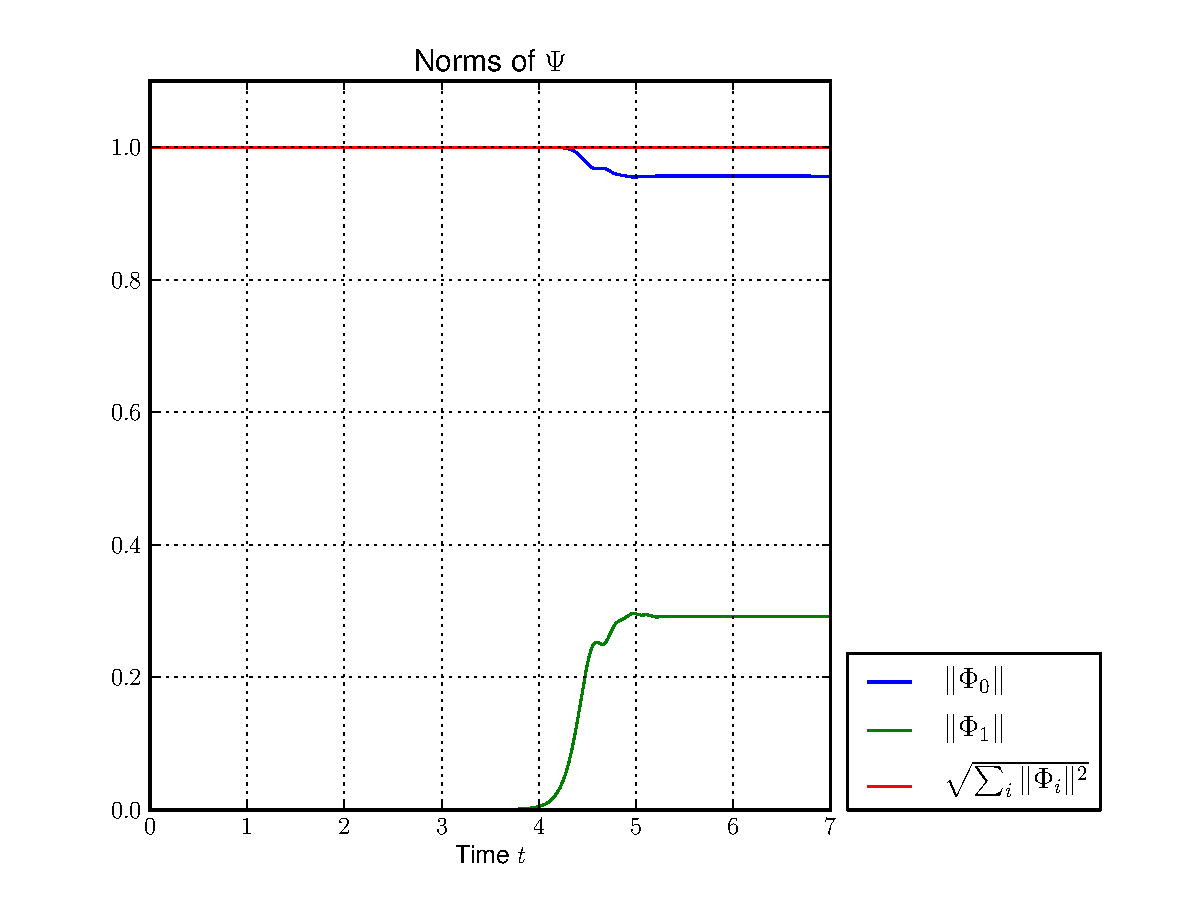
\includegraphics[width=0.5\linewidth]{./figures/delta_gap_phi2phi3/norms_block0.pdf}
  }
  \subfloat[][]{
    \label{fig:basic_delta_gap_phi2phi3_norms_drift}
    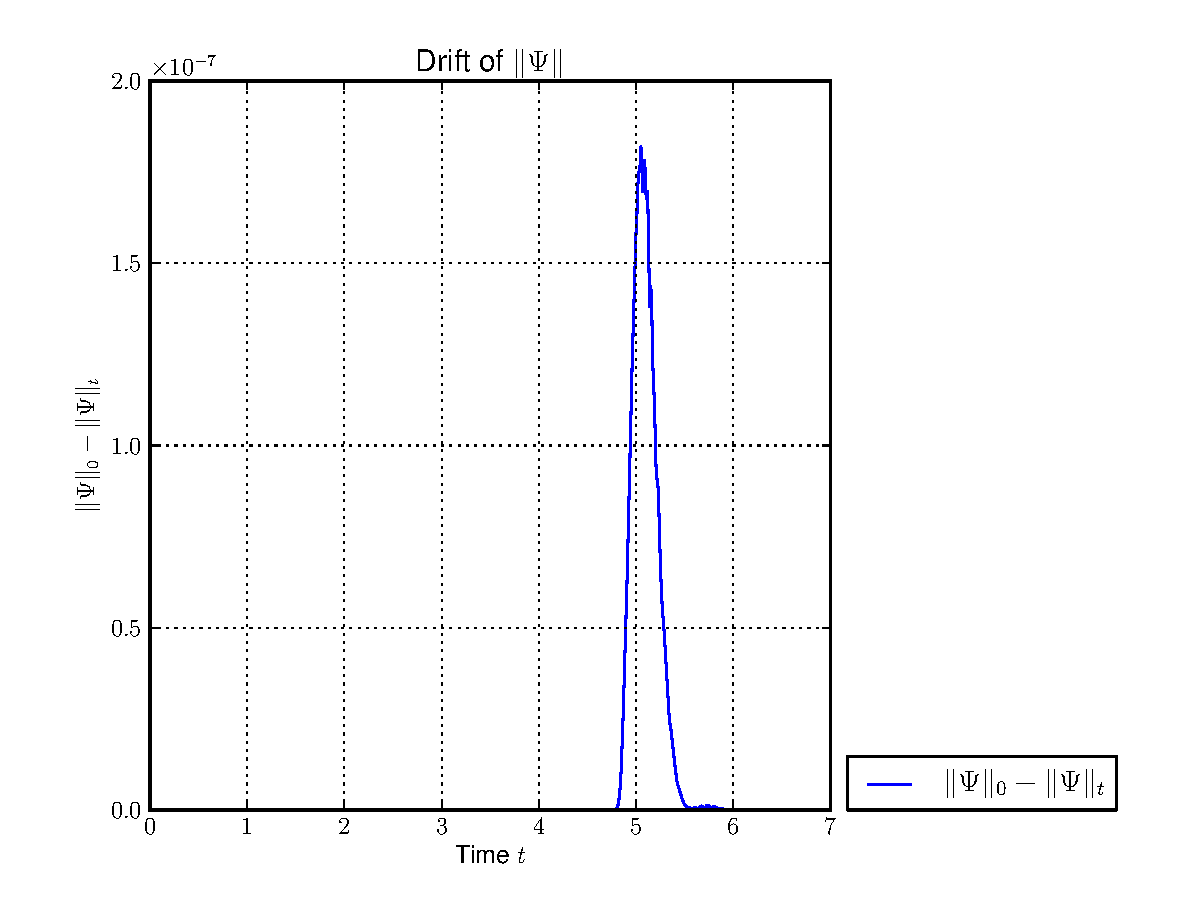
\includegraphics[width=0.5\linewidth]{./figures/delta_gap_phi2phi3/norms_drift_block0.pdf}
  } \\
  \caption[Norms and norm drift for a superposition $\phi_2+\phi_3$ in an avoided crossing]{
  This figure shows the norm of both components $\Phi_0$ and $\Phi_1$ of the
  wavepacket $\Psi$ as well as the overall norm. The right panel shows the drift
  of the overall norm, which should be conserved as good as possible.
  The initial wavepacket $\Ket{\Psi\ofs{t=0}} = \phi_2 + \phi_3$ starts on the
  upper level. The full set of simulation parameters is printed in \ref{cfg:delta_gap_phi2phi3}
  \label{fig:basic_delta_gap_phi2phi3_norms}
  }
\end{figure}


\begin{figure}[h!]
  \centering
  \subfloat[][]{
    \label{fig:basic_delta_gap_phi2phi3_energy}
    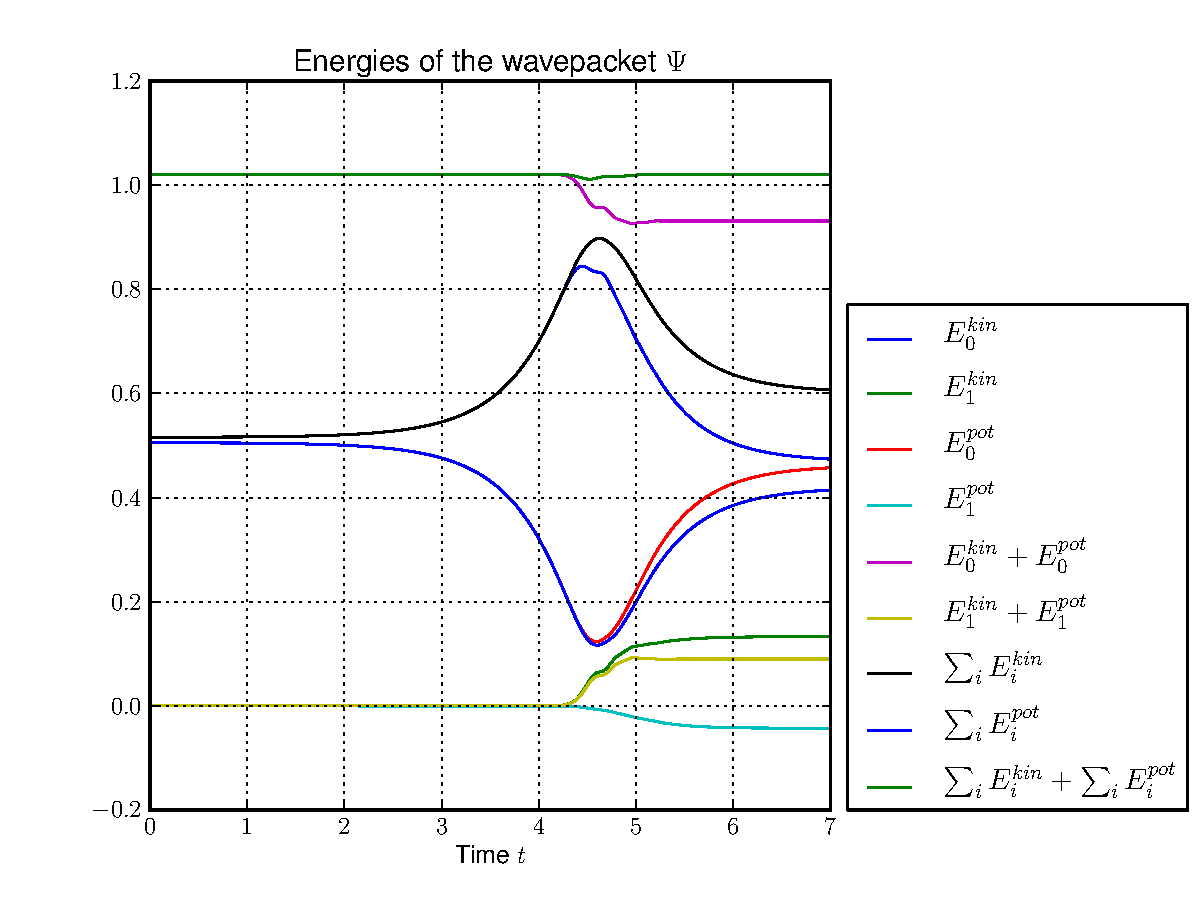
\includegraphics[width=0.5\linewidth]{./figures/delta_gap_phi2phi3/energies_block0.pdf}
  }
  \subfloat[][]{
    \label{fig:basic_delta_gap_phi2phi3_energy_drift}
    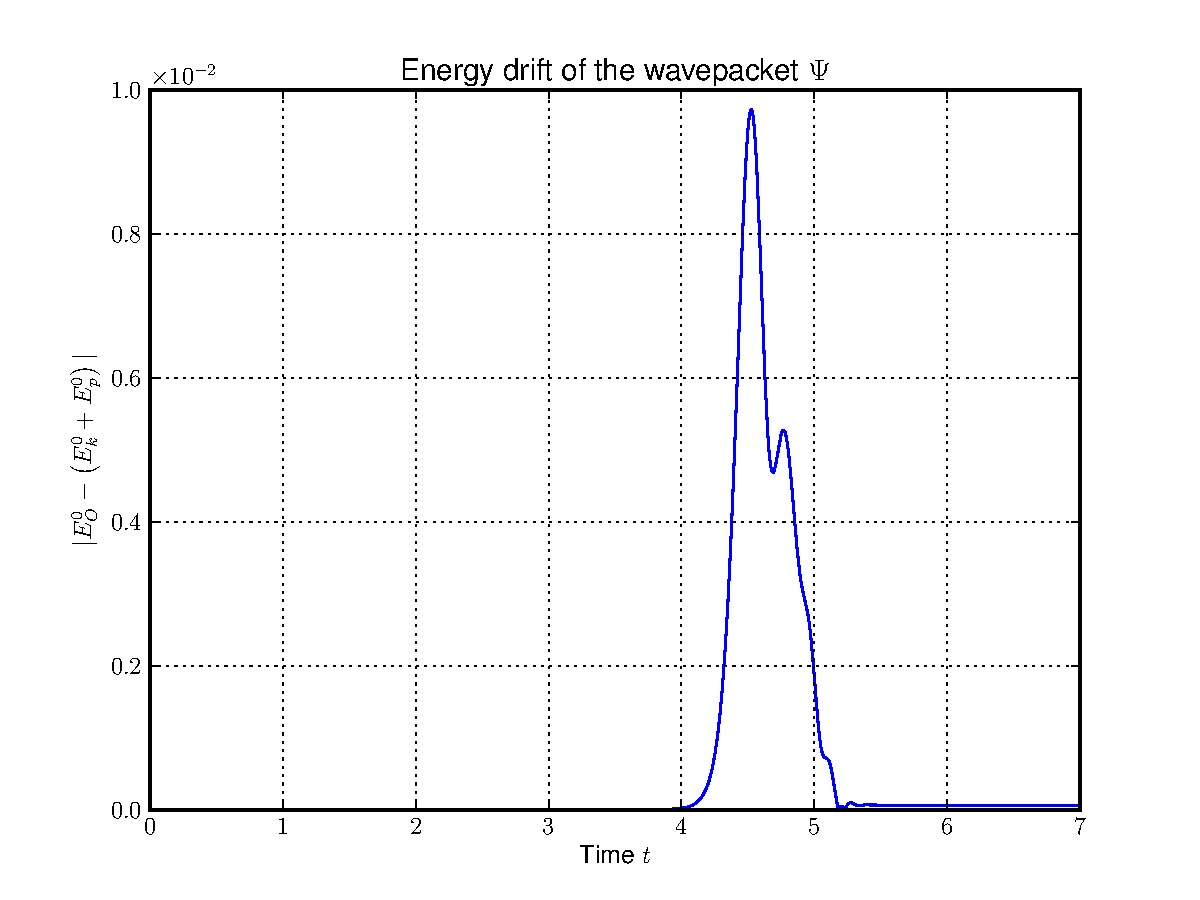
\includegraphics[width=0.5\linewidth]{./figures/delta_gap_phi2phi3/energy_drift_block0.pdf}
  } \\
  \caption[Energies for a superposition of $\phi_2$ and $\phi_3$ in an avoided crossing]{
  Kinetic and potential energies and the violation of energy conservation for an
  initial superposition of $\phi_2$ and $\phi_3$ starting on the upper level. The
  full set of simulation parameters is printed in \ref{cfg:delta_gap_phi2phi3}
  \label{fig:basic_delta_gap_phi2phi3_energies}
  }
\end{figure}


\FloatBarrier
\section{Aposteriori spawning for avoided crossings}

The aposteriori spawning process for avoided crossings can be described by the
general algorithm \ref{al:aposteriori_spawning}. The only difference to the tunneling
case are the input values. First we deal with vector values packets $\Psi$ consisting
of $N$ components in the general case. And we concentrate not on a subset of $\Phi_0$
but on a whole $\Phi_i$. Hence the values for $\alpha$ and $\beta$ must be set
to $0$ and $K-1$ to obtain the correct fragment $w$. We set the input value $\nu$
to the component we wish to monitor. In the simulation above where we have only two
energy levels ($N=2$) and start on the upper one this would be the lower level
and thus $\nu = 1$.

The following examples show the aposteriori spawning process based on the simulations
from the last section. The gap size $\delta$ of the avoided crossing is chosen in
a way that if we start which a $\phi_i$ on the upper level then we end up again
with a $\phi^\prime_i$ on the lower level, for details see reference \cite{BGH_natac}.
We first look at the norms and the energies. The most important observation here is that
the results crucially depend on the values of $k$ in the formula \eqref{eq:estimate_abssqrPQ}.
If we just set $k=0$ we get wrong norms and wrong energies for higher order
$\phi_i$. This can be seen in the following figures. In \ref{fig:spawn_delta_gap_norms1}
and \ref{fig:spawn_delta_gap_norms2} the orange curve is the norm of the original
part $\Phi_1$ on the lower level. And the cyan curve should match as good as possible.
Also in figures \ref{fig:spawn_delta_gap_norms_drift1} and \ref{fig:spawn_delta_gap_norms_drift2}
we observe that for $k=0$ (left panels) the error in the norm conservation of
$\Phi_1$ differs considerably from what we have in the right panels where
the norm conservation is fulfilled again after the avoided crossing.
For the kinetic and potential energies of $\Phi_1$ we have a similar picture.
Figures \ref{fig:spawn_delta_gap_energies1} and \ref{fig:spawn_delta_gap_energies2}
show various energies. The kinetic energy of the original wavepacket's components
$\Phi_0$ and $\Phi_1$ is plotted in red, the potential energy in orange. The cyan
and light green curves overlap these two only for the compatible choice of $k$.
We should note that in either case we get good results only \emph{after} the
packet passed the avoided crossing. This compares to the tunneling case where
spawning a new packet makes only sense after tunneling has already occurred.
The energy conservation shown in figures \ref{fig:spawn_delta_gap_energy_drift1}
and \ref{fig:spawn_delta_gap_energy_drift2} is violated heavily after the crossing
for $k=0$ but fulfilled quite well for the matching choice of $k$.
In summary we find that the values from the original simulation and the
corresponding ones from the aposteriori simulations do not overlap if $k$
does not match to the $\phi_k$, sometimes not even for asymptotic large
times. So the algorithm does not converge in these cases.


\begin{figure}
  \centering
  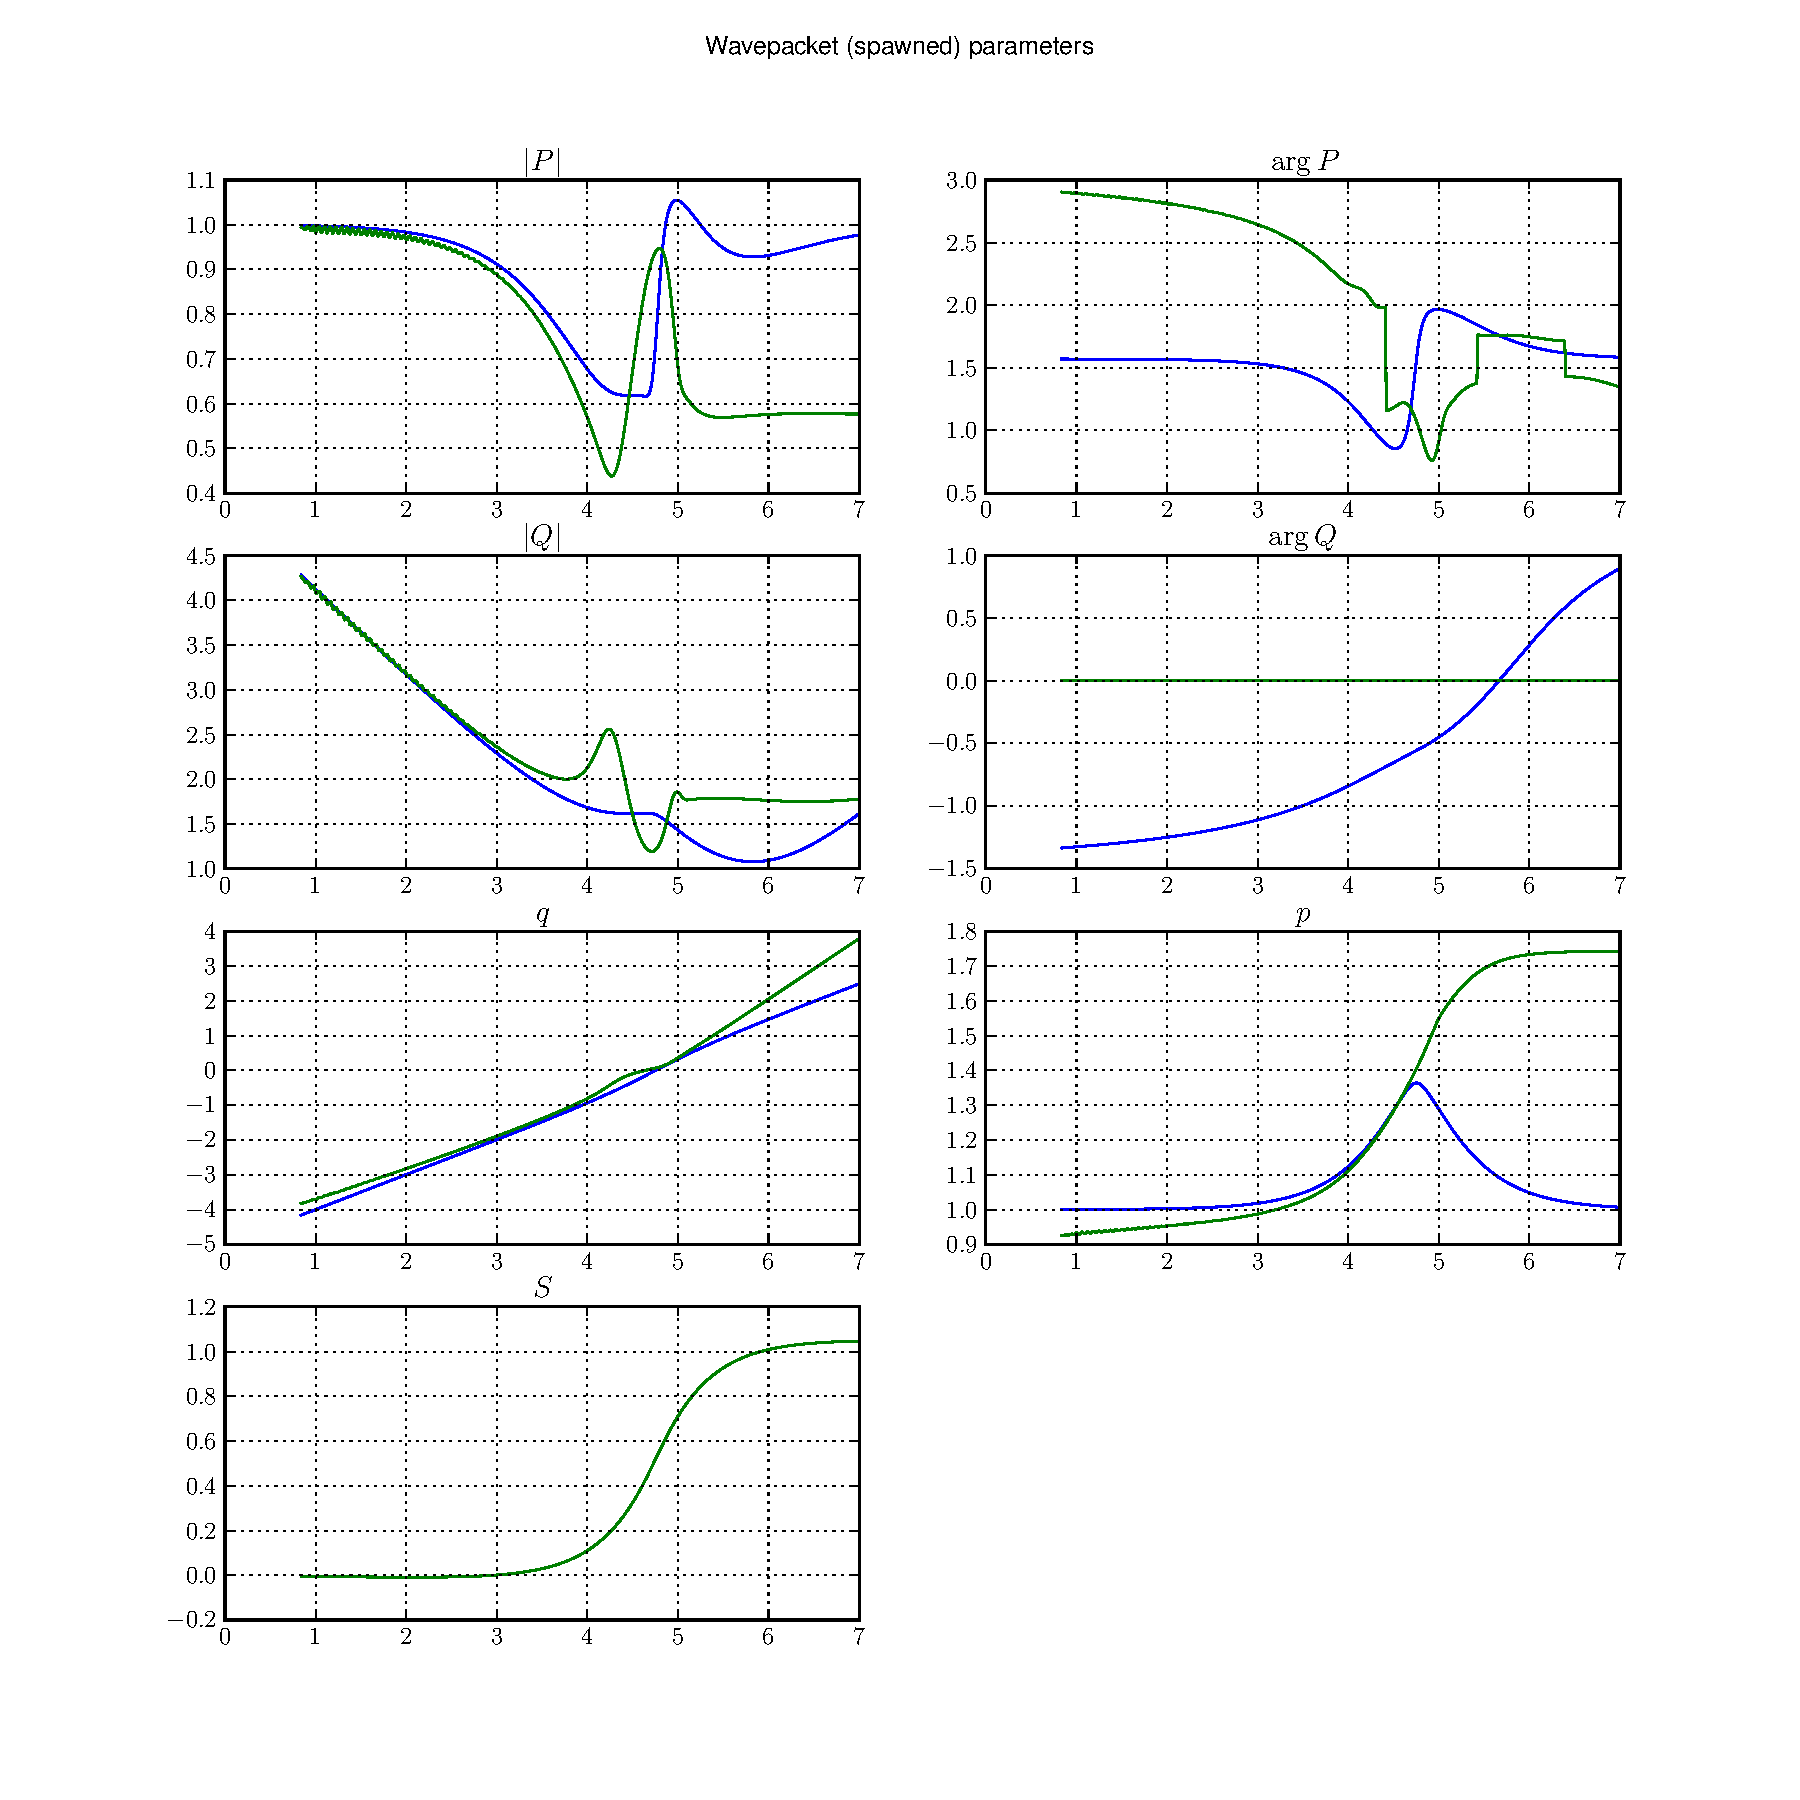
\includegraphics[width=\the\linewidth]{./figures/delta_gap_spawn_phi0_k0/wavepacket_parameters_abs_ang_spawned.pdf}
  \caption[The parameter sets $\Pi$ (blue) and $\tilde{\Pi}$ (green) for the case of
  $\Psi = \phi_0$ and $k=0$]{The parameter sets $\Pi$ (blue) and $\tilde{\Pi}$ (green) for the case of
  $\Psi = \phi_0$ and $k=0$. We can give a nice interpretation to the parameters
  $\tilde{q}$ and $\tilde{p}$. For $\tilde{q}$ we see a steeper slope which means
  that after the crossing the spawned packet on the lower level moves faster. And
  $\tilde{p}$ continues to increase after the crossing while $p$ becomes smaller
  again which seems right compared to the shape of the potential.
  The full set of simulation parameters is printed in \ref{cfg:delta_gap_apost_phi0_k0}.
  }
  \label{fig:avoided_crossing_parameters}
\end{figure}


\begin{figure}[h!]
  \centering
  \subfloat[][]{
    \label{fig:spawn_delta_gap_phi1_k0_norms}
    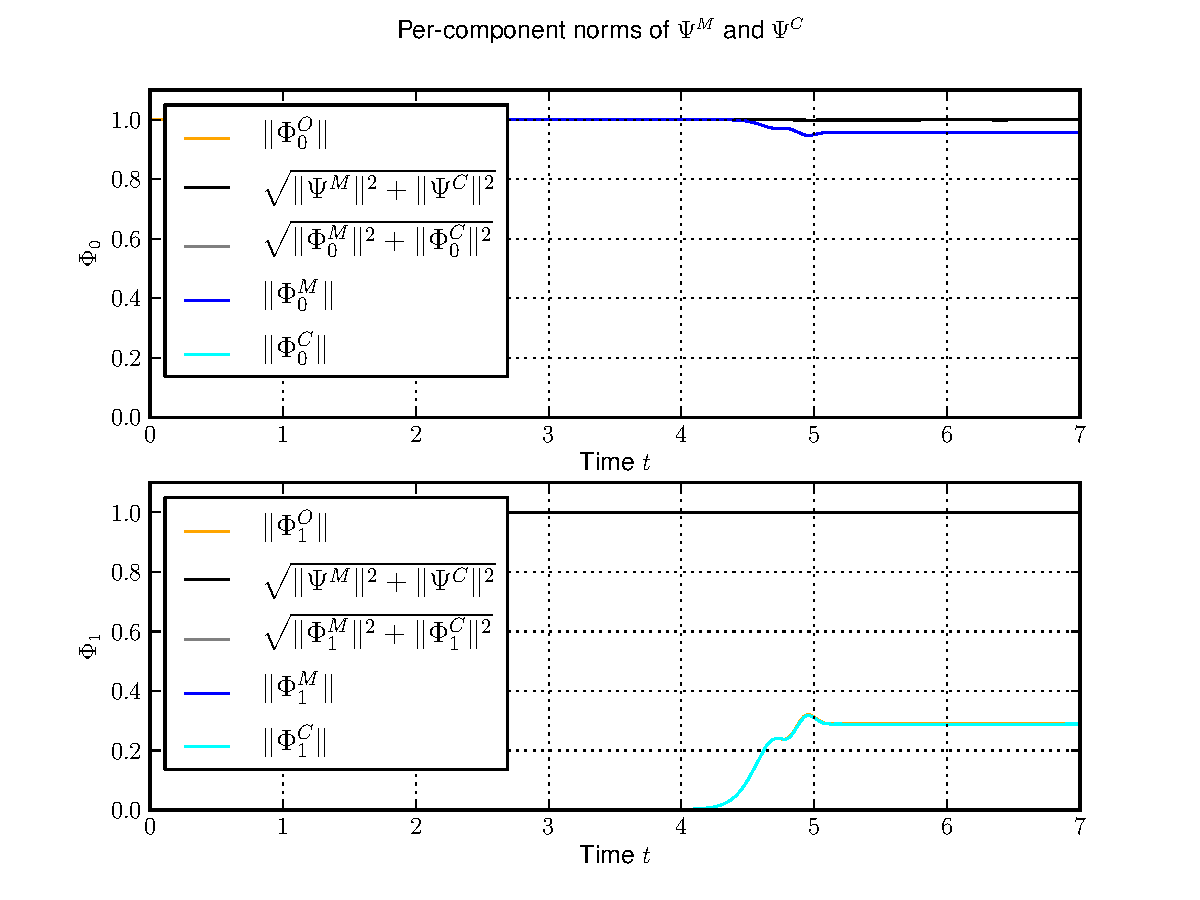
\includegraphics[width=0.5\linewidth]{./figures/delta_gap_spawn_phi1_k0/norms_compare_components_group0.pdf}
  }
  \subfloat[][]{
    \label{fig:spawn_delta_gap_phi1_k1_norms}
    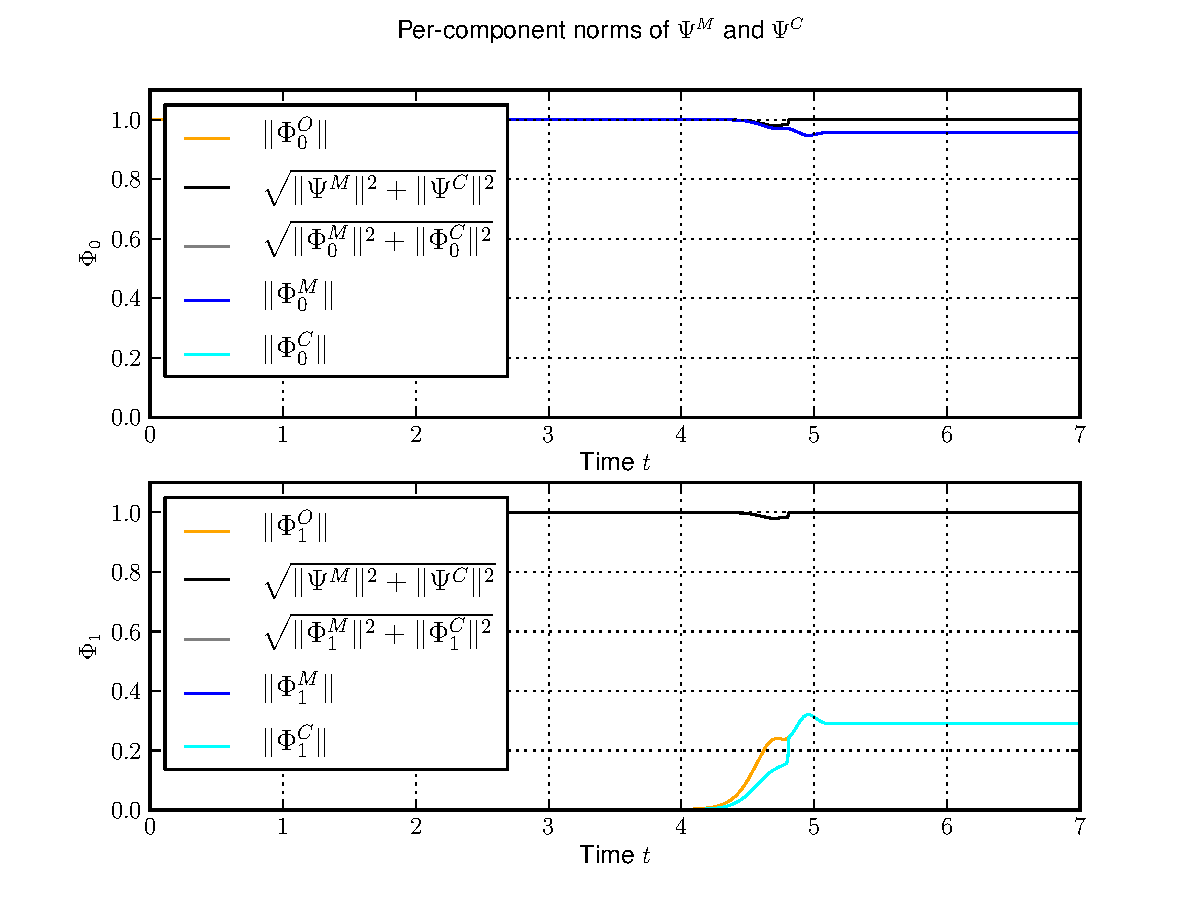
\includegraphics[width=0.5\linewidth]{./figures/delta_gap_spawn_phi1_k1/norms_compare_components_group0.pdf}
  } \\
  \subfloat[][]{
    \label{fig:spawn_delta_gap_phi2_k0_norms}
    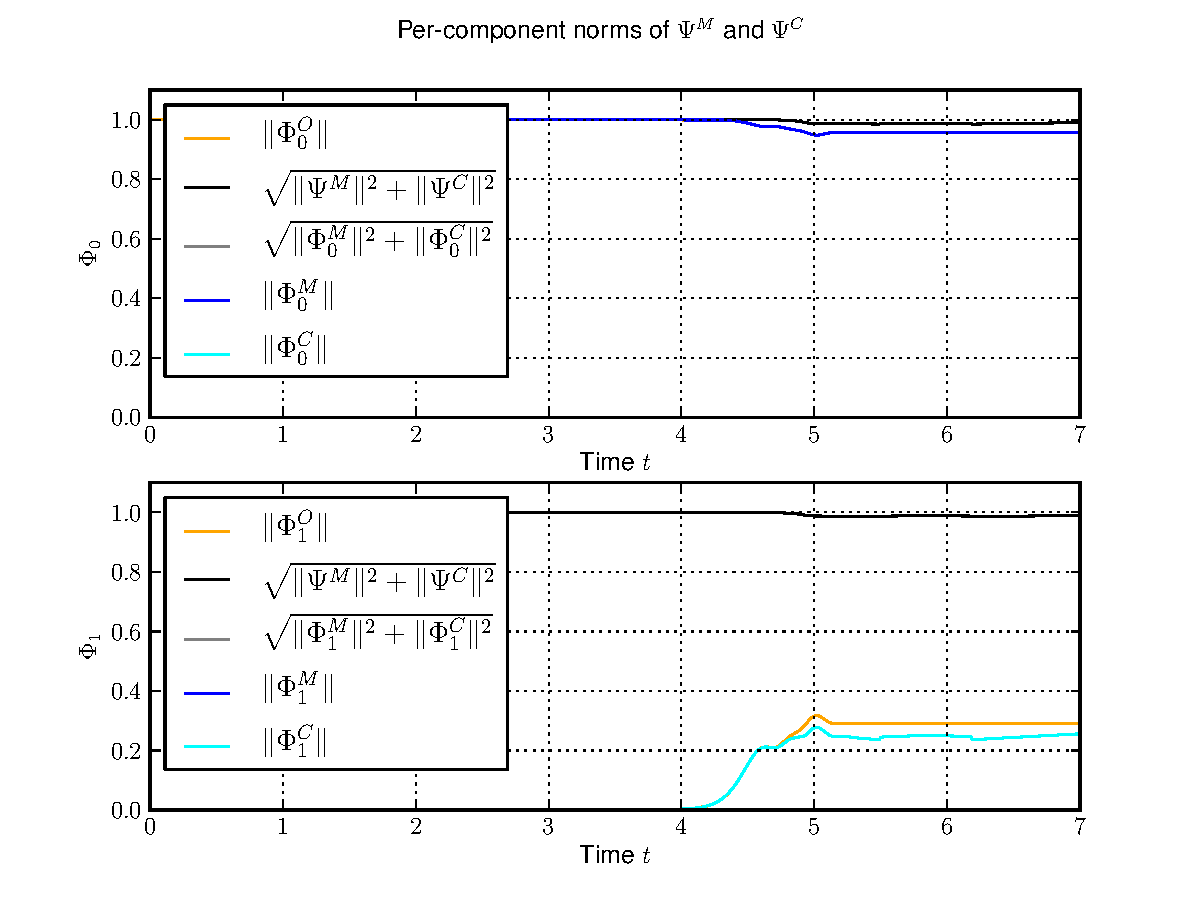
\includegraphics[width=0.5\linewidth]{./figures/delta_gap_spawn_phi2_k0/norms_compare_components_group0.pdf}
  }
  \subfloat[][]{
    \label{fig:spawn_delta_gap_phi2_k2_norms}
    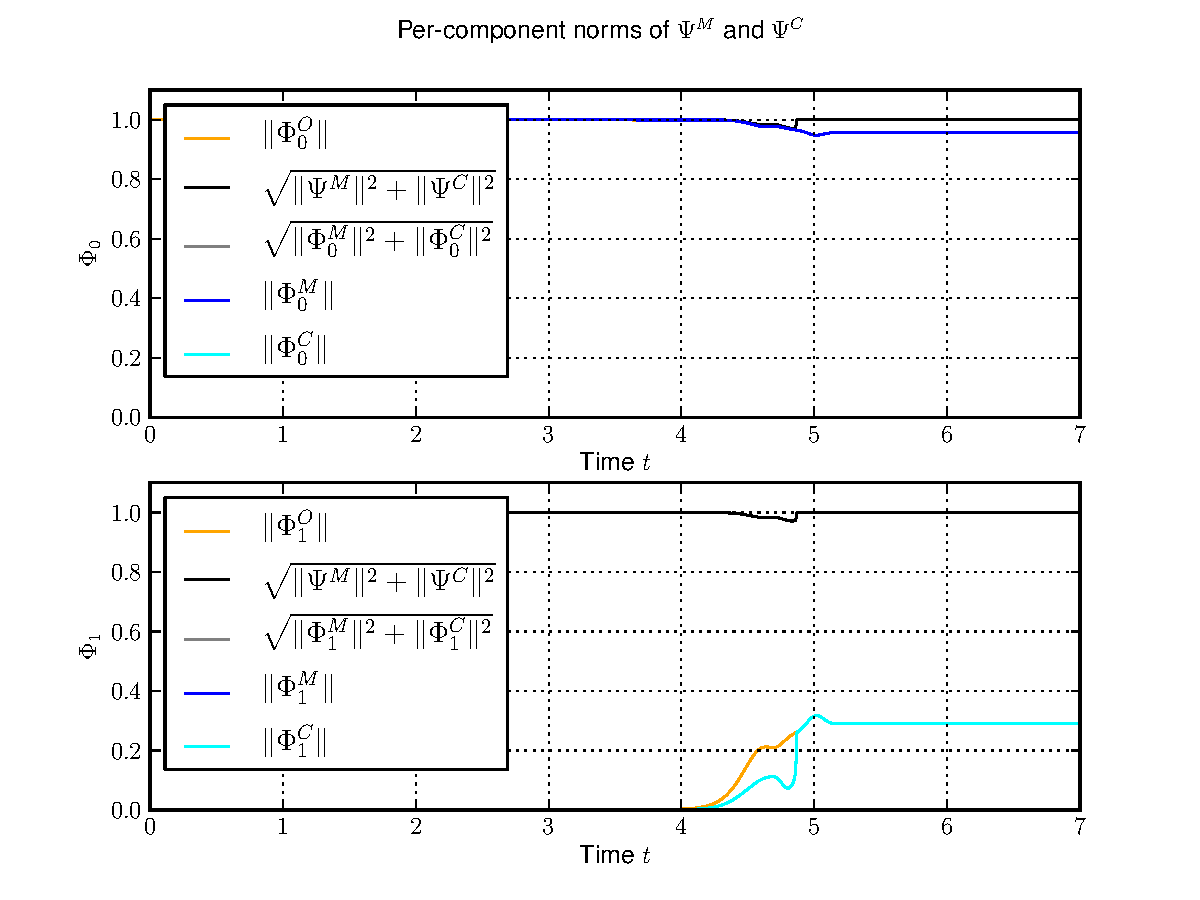
\includegraphics[width=0.5\linewidth]{./figures/delta_gap_spawn_phi2_k2/norms_compare_components_group0.pdf}
  } \\
  \subfloat[][]{
    \label{fig:spawn_delta_gap_phi3_k0_norms}
    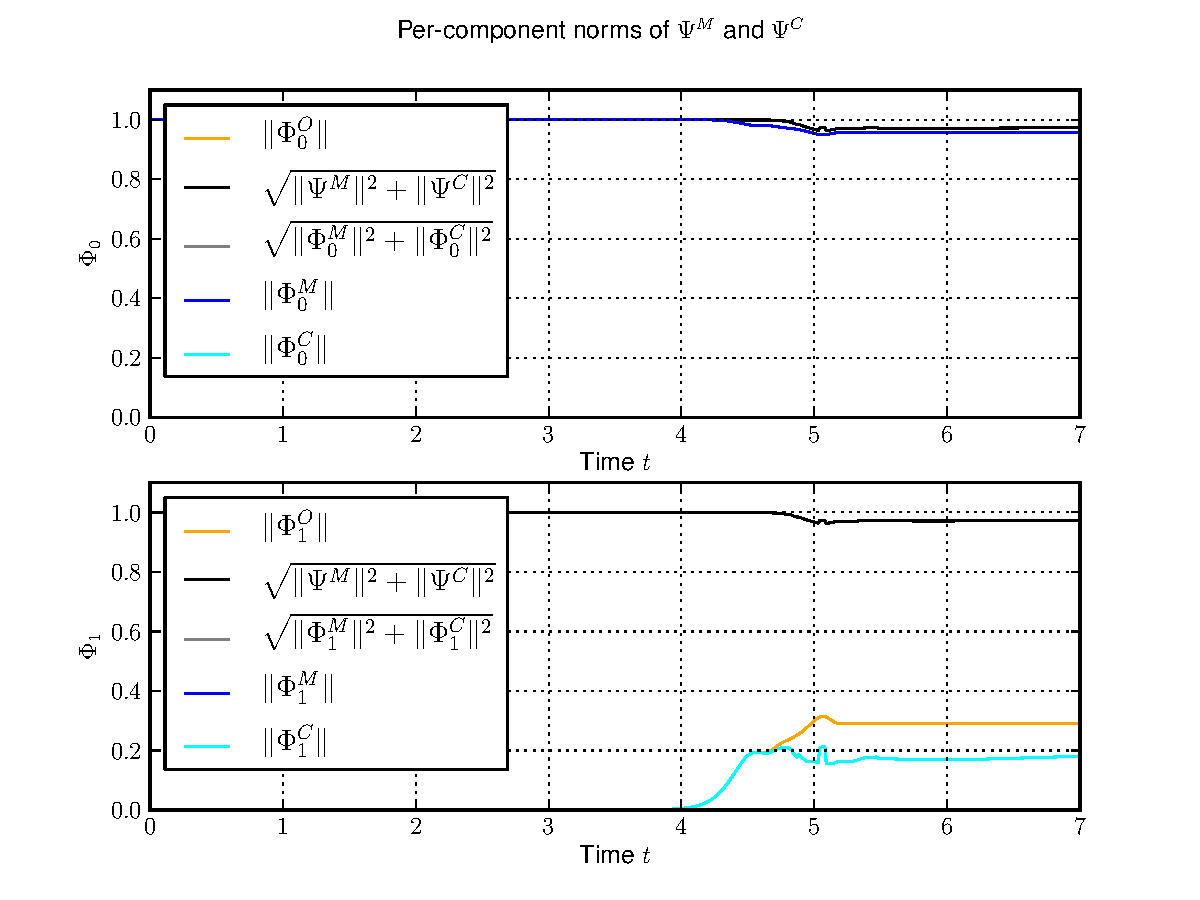
\includegraphics[width=0.5\linewidth]{./figures/delta_gap_spawn_phi3_k0/norms_compare_components_group0.pdf}
  }
  \subfloat[][]{
    \label{fig:spawn_delta_gap_phi3_k3_norms}
    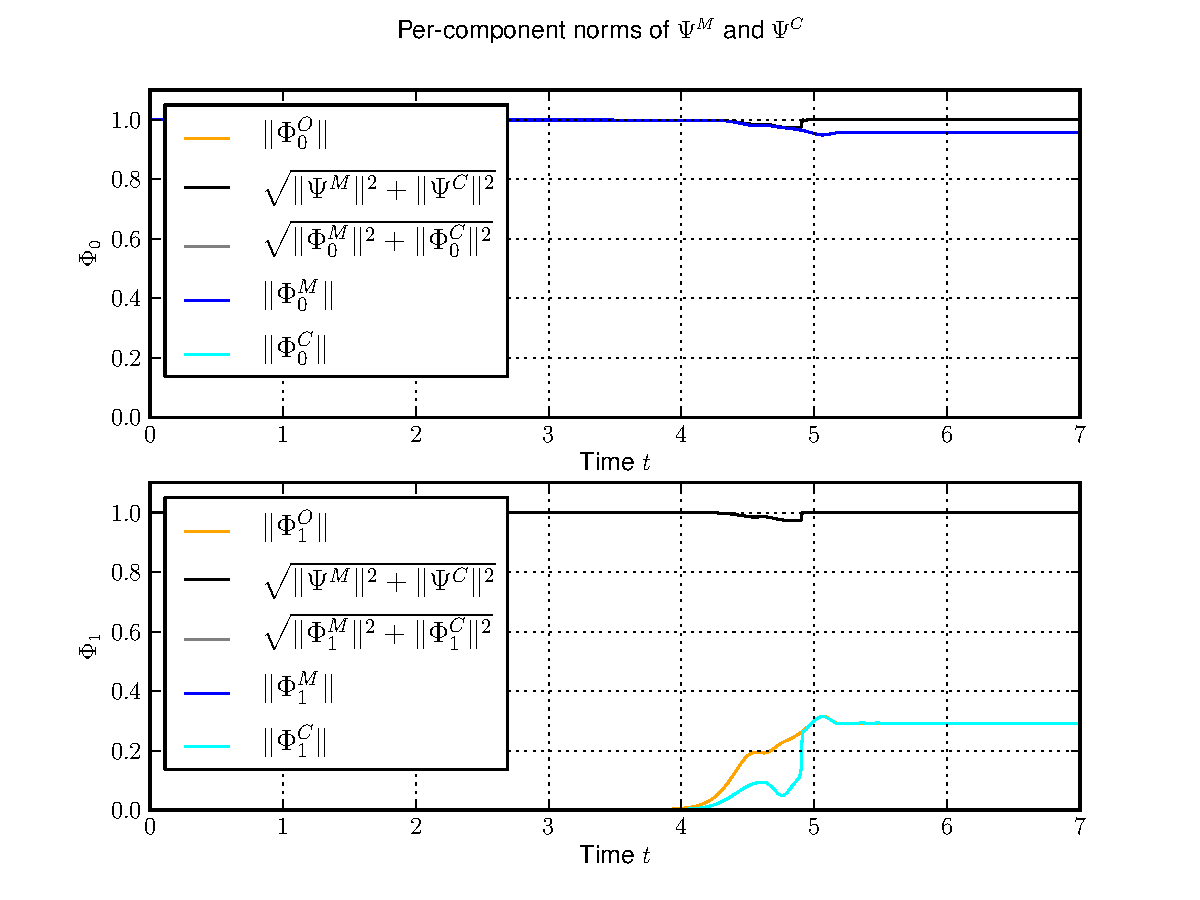
\includegraphics[width=0.5\linewidth]{./figures/delta_gap_spawn_phi3_k3/norms_compare_components_group0.pdf}
  } \\
  \caption[The norms for several non-adiabatic examples]{
  This figure shows the component-wise norms for several non-adiabatic examples.
  The individual panels are for different wavepackets $\Psi = \phi_i$ and different
  values of $k$ where the $k$ is the one from formula \eqref{eq:estimate_abssqrPQ}.
  The full set of simulation parameters is printed in \ref{cfg:delta_gap_apost}.
  \subref{fig:spawn_delta_gap_phi1_k0_norms} $\Psi = \phi_1$ and $k=0$
  \subref{fig:spawn_delta_gap_phi1_k1_norms} $\Psi = \phi_1$ and $k=1$
  \subref{fig:spawn_delta_gap_phi2_k0_norms} $\Psi = \phi_2$ and $k=0$
  \subref{fig:spawn_delta_gap_phi2_k2_norms} $\Psi = \phi_2$ and $k=2$
  \subref{fig:spawn_delta_gap_phi3_k0_norms} $\Psi = \phi_3$ and $k=0$
  \subref{fig:spawn_delta_gap_phi3_k3_norms} $\Psi = \phi_3$ and $k=3$
  \label{fig:spawn_delta_gap_norms1}
  }
\end{figure}


\begin{figure}[h!]
  \centering
  \subfloat[][]{
    \label{fig:spawn_delta_gap_phi4_k0_norms}
    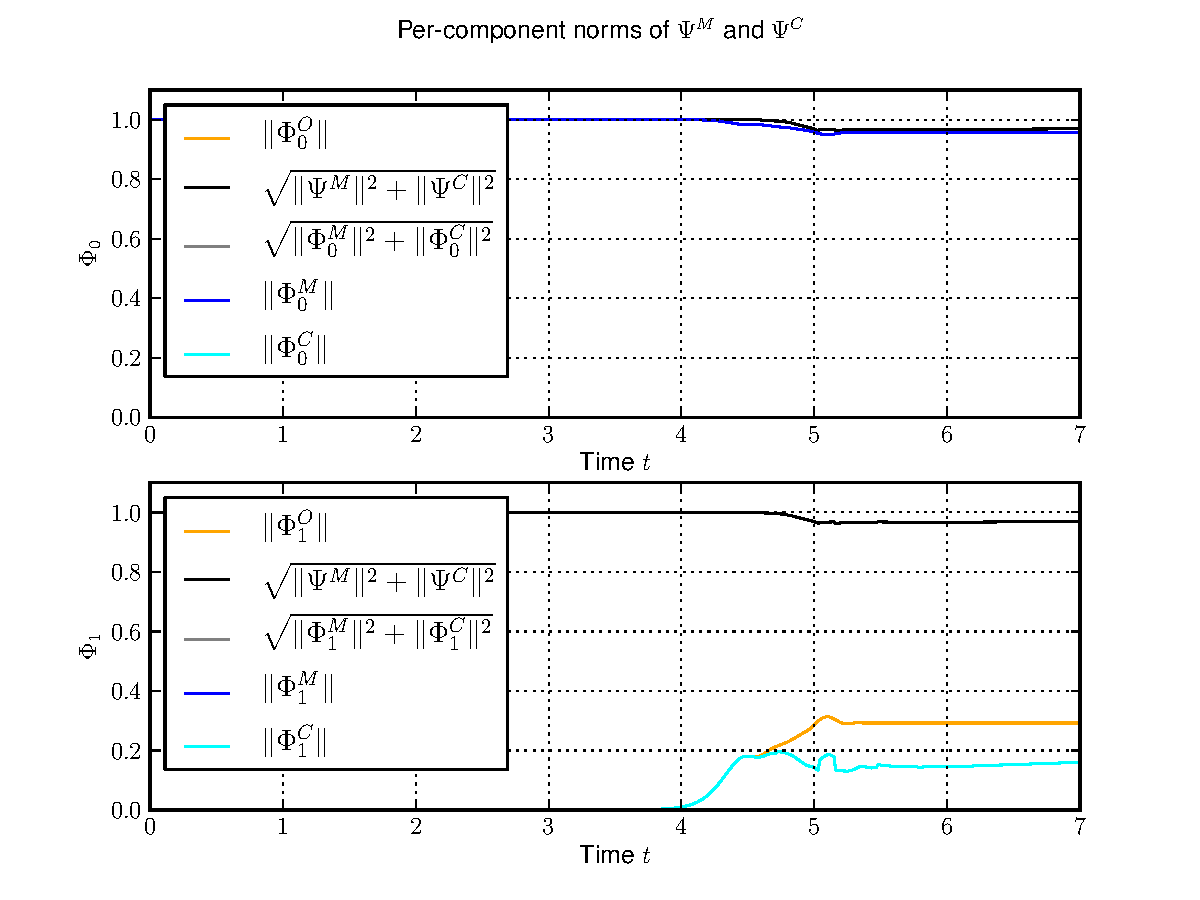
\includegraphics[width=0.5\linewidth]{./figures/delta_gap_spawn_phi4_k0/norms_compare_components_group0.pdf}
  }
  \subfloat[][]{
    \label{fig:spawn_delta_gap_phi4_k4_norms}
    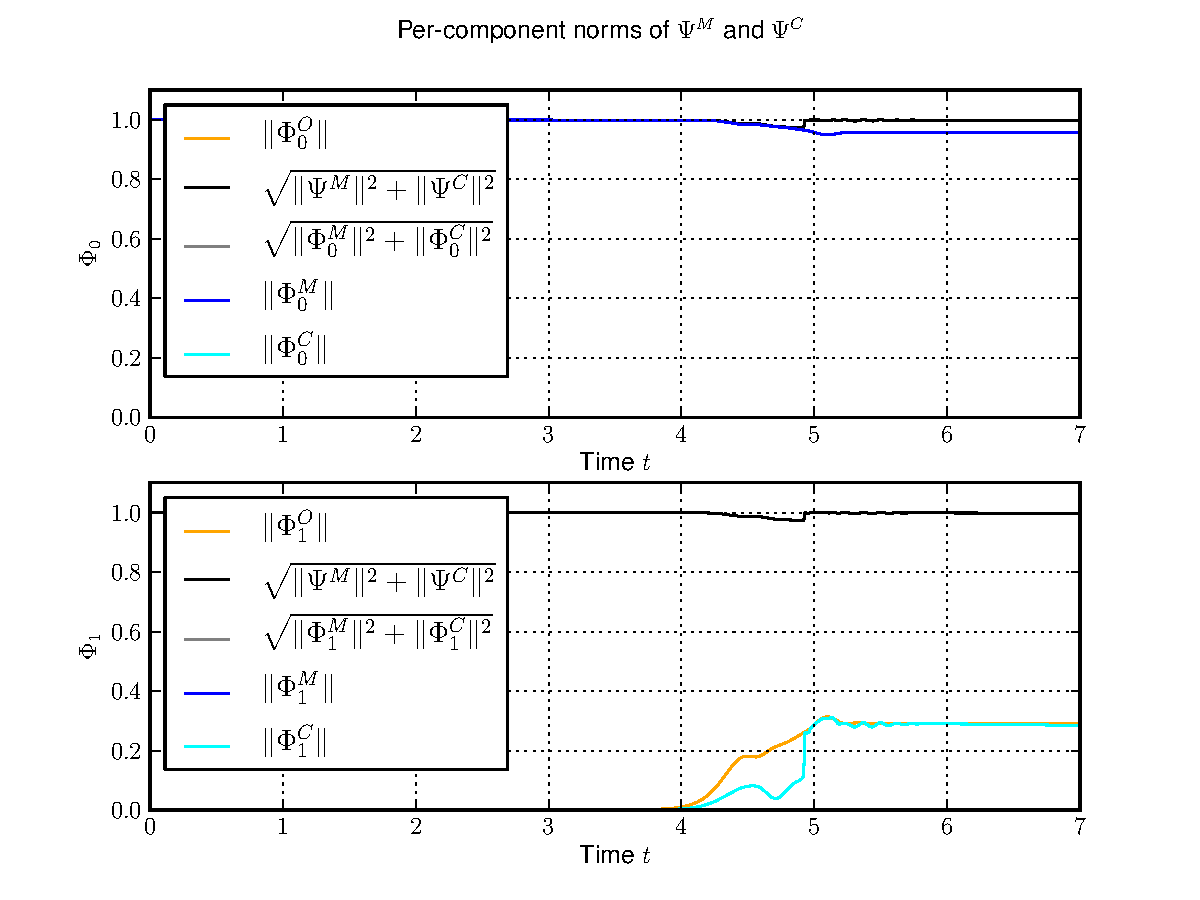
\includegraphics[width=0.5\linewidth]{./figures/delta_gap_spawn_phi4_k4/norms_compare_components_group0.pdf}
  } \\
  \subfloat[][]{
    \label{fig:spawn_delta_gap_phi0phi1_k0_norms}
    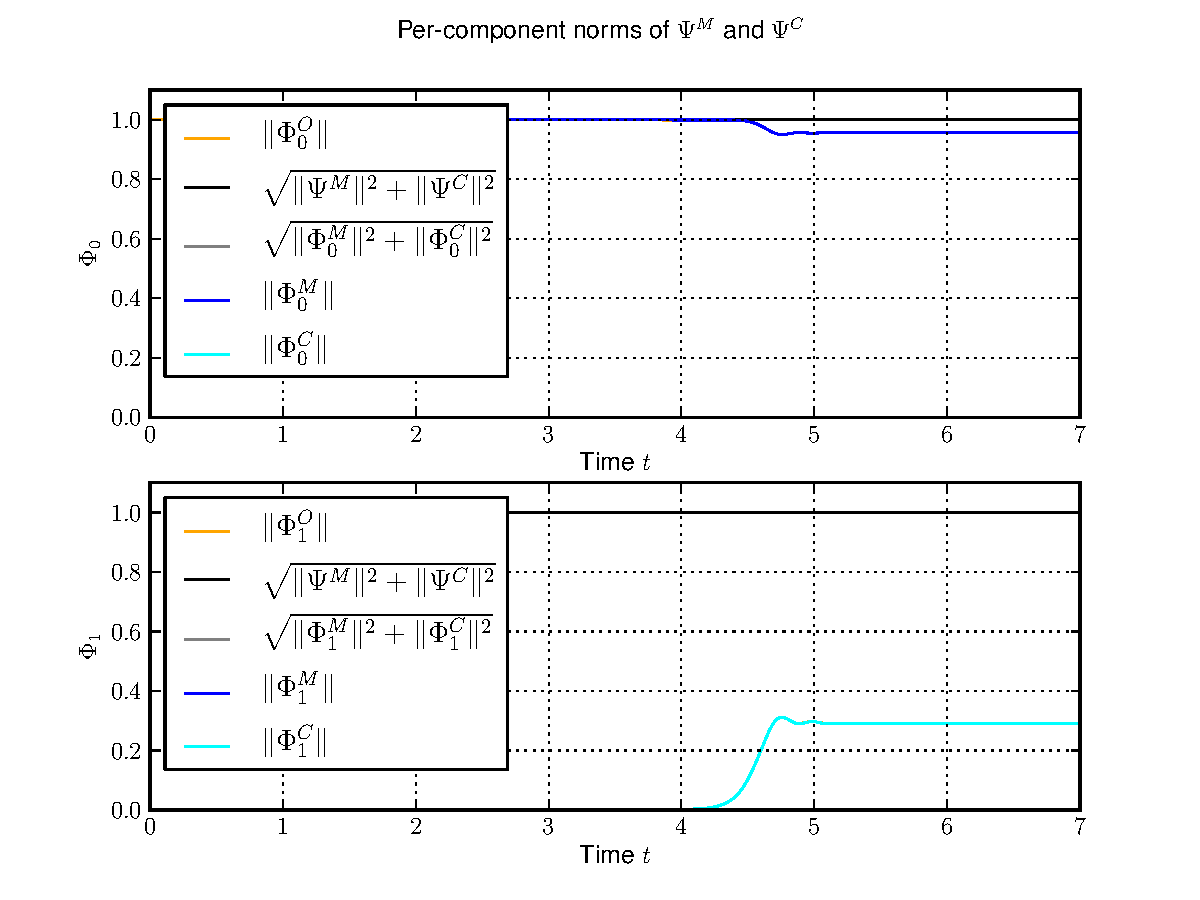
\includegraphics[width=0.5\linewidth]{./figures/delta_gap_spawn_phi0phi1_k0/norms_compare_components_group0.pdf}
  }
  \subfloat[][]{
    \label{fig:spawn_delta_gap_phi2phi3_k0_norms}
    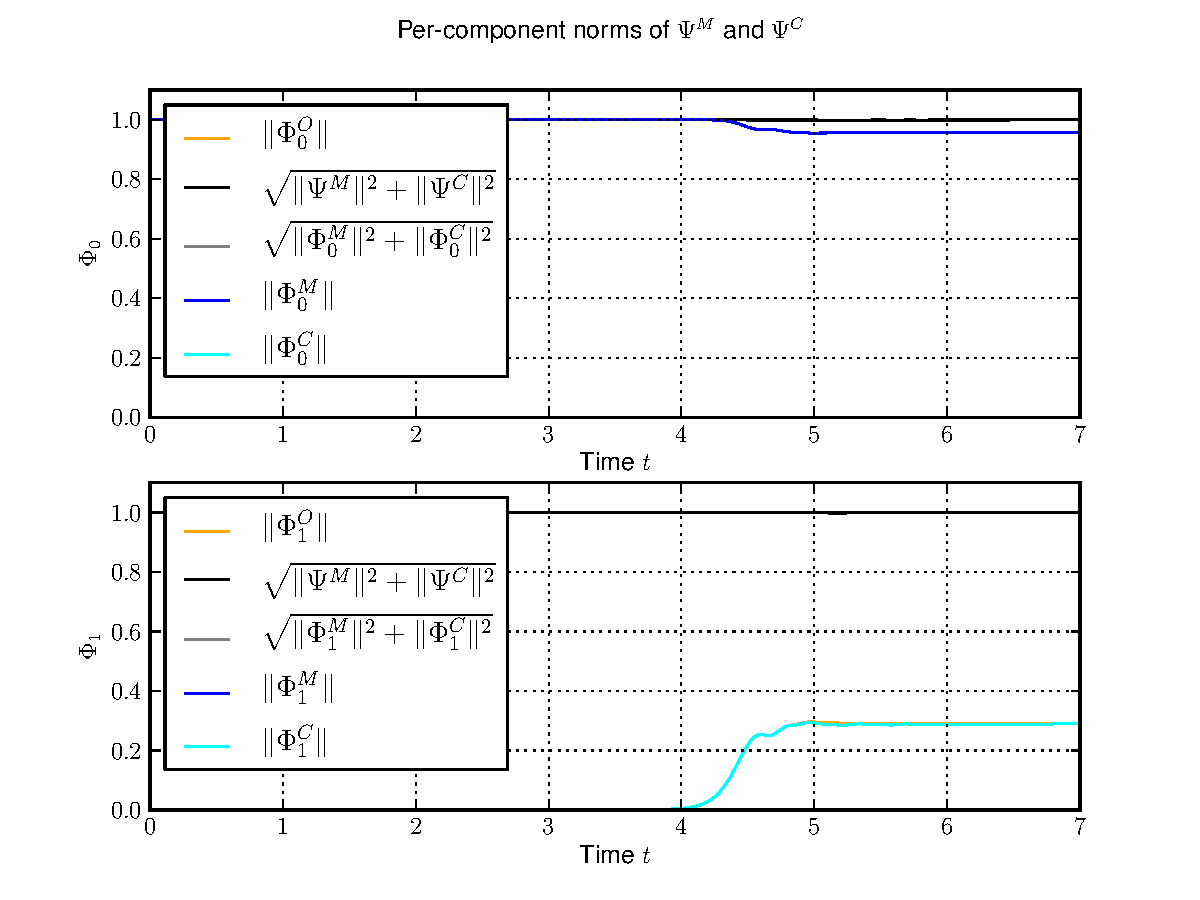
\includegraphics[width=0.5\linewidth]{./figures/delta_gap_spawn_phi2phi3_k0/norms_compare_components_group0.pdf}
  } \\
  \subfloat[][]{
    \label{fig:spawn_delta_gap_phi0_k0_norms}
    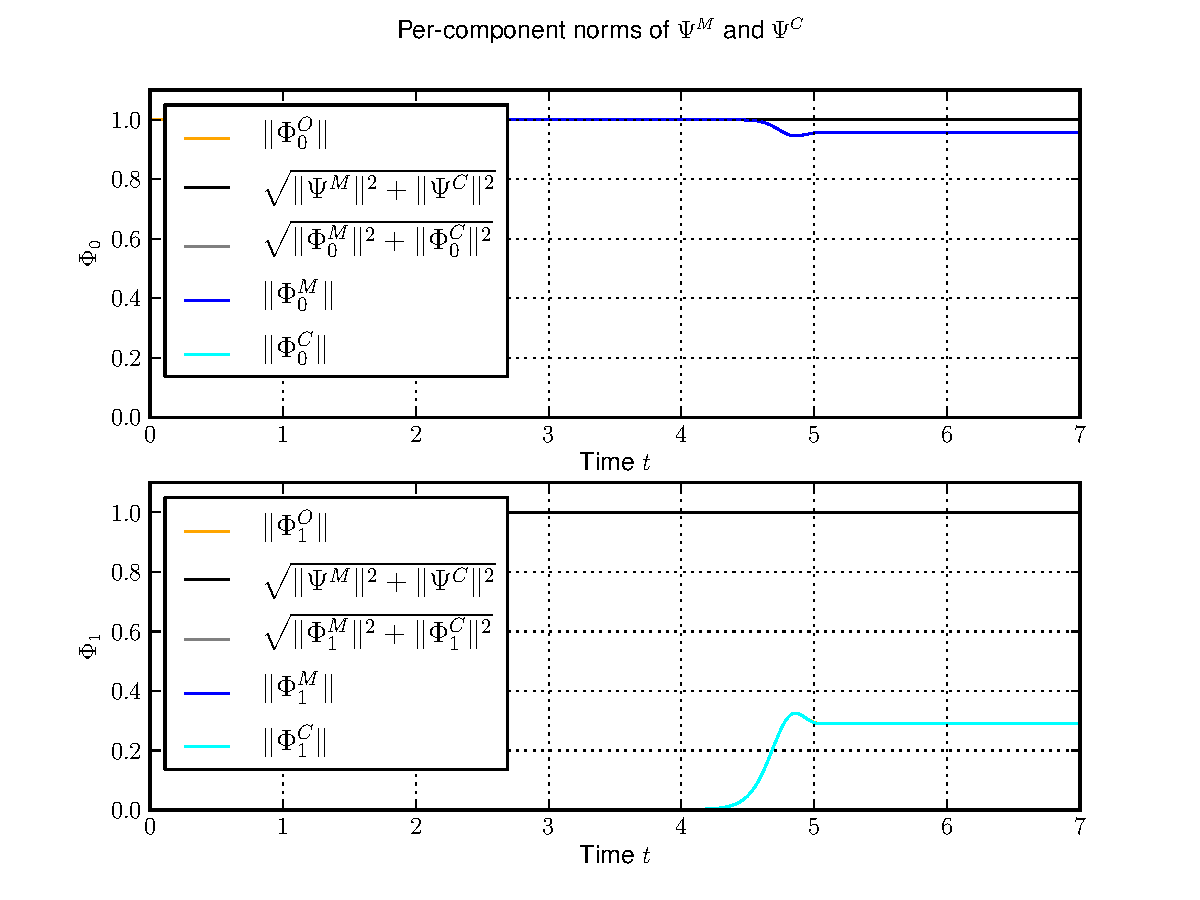
\includegraphics[width=0.5\linewidth]{./figures/delta_gap_spawn_phi0_k0/norms_compare_components_group0.pdf}
  } \\
  \caption[The norms for several non-adiabatic examples]{
  This figure shows the component-wise norms for several non-adiabatic examples.
  The individual panels are for different wavepackets $\Psi = \phi_i$ and different
  values of $k$ where the $k$ is the one from formula \eqref{eq:estimate_abssqrPQ}.
  The full set of simulation parameters is printed in \ref{cfg:delta_gap_apost}.
  \subref{fig:spawn_delta_gap_phi4_k0_norms} $\Psi = \phi_4$ and $k=0$
  \subref{fig:spawn_delta_gap_phi4_k4_norms} $\Psi = \phi_4$ and $k=4$
  \subref{fig:spawn_delta_gap_phi0phi1_k0_norms} $\Psi = \phi_0 + \phi_1$ and $k=0$
  \subref{fig:spawn_delta_gap_phi2phi3_k0_norms} $\Psi = \phi_2 + \phi_3$ and $k=0$
  \subref{fig:spawn_delta_gap_phi0_k0_norms} $\Psi = \phi_0$ and $k=0$
  \label{fig:spawn_delta_gap_norms2}
  }
\end{figure}



\begin{figure}[h!]
  \centering
  \subfloat[][]{
    \label{fig:spawn_delta_gap_phi1_k0_norms_drift}
    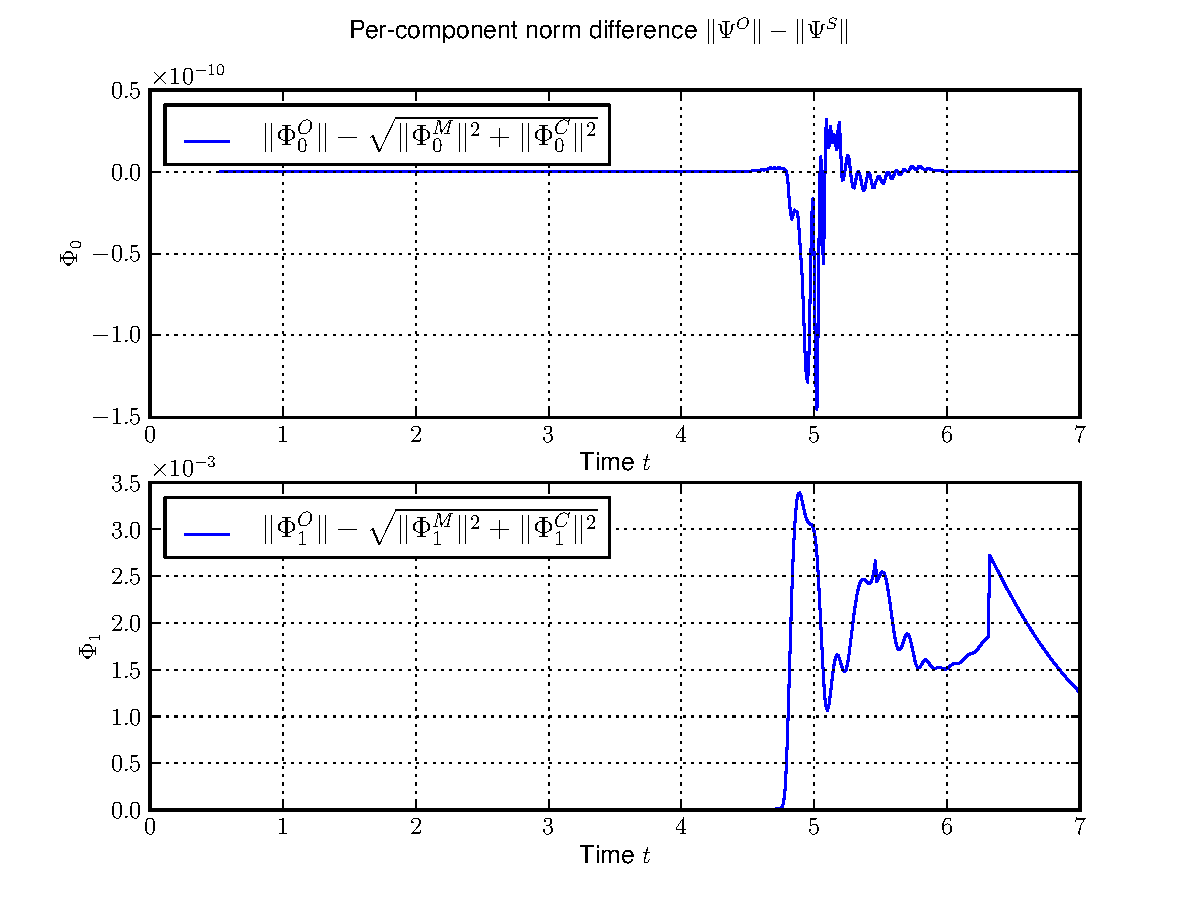
\includegraphics[width=0.5\linewidth]{./figures/delta_gap_spawn_phi1_k0/norms_compare_components_diff_group0.pdf}
  }
  \subfloat[][]{
    \label{fig:spawn_delta_gap_phi1_k1_norms_drift}
    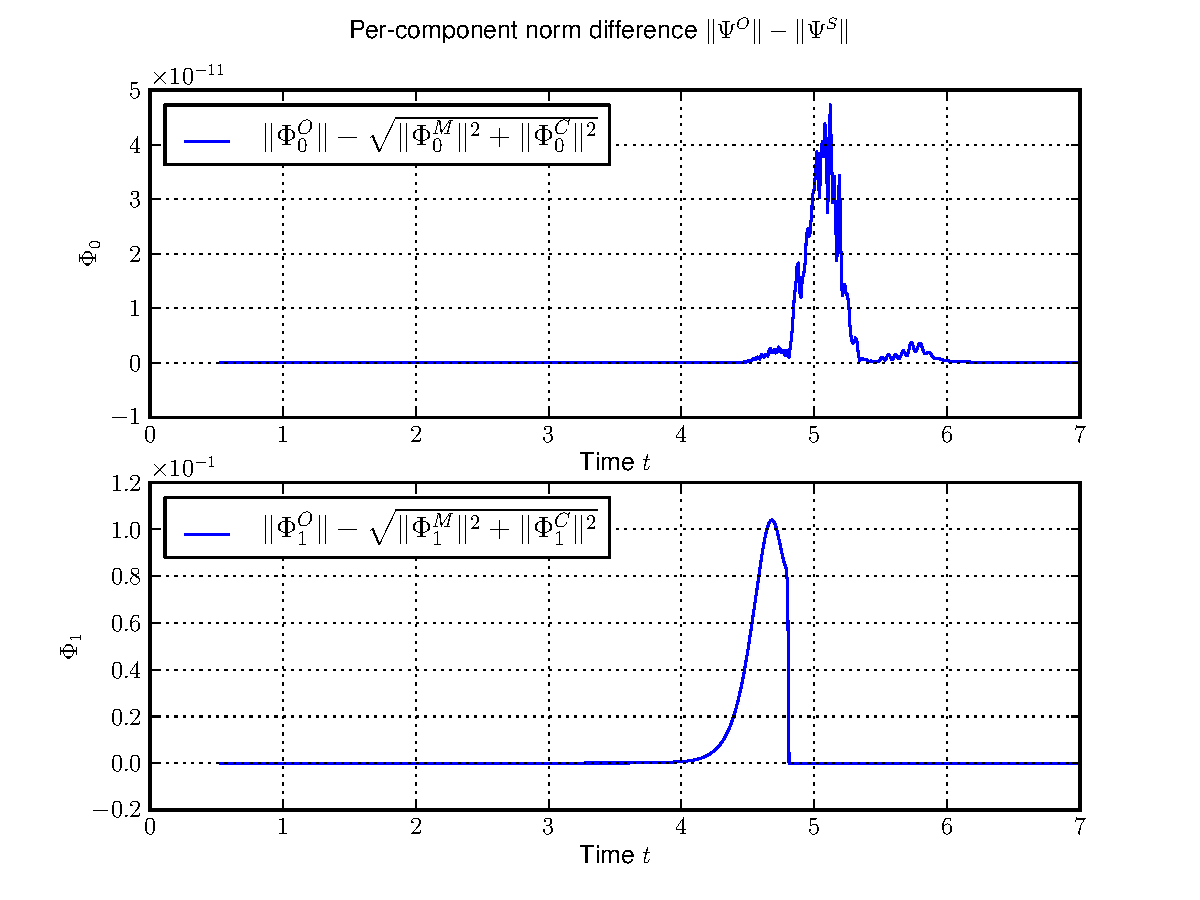
\includegraphics[width=0.5\linewidth]{./figures/delta_gap_spawn_phi1_k1/norms_compare_components_diff_group0.pdf}
  } \\
  \subfloat[][]{
    \label{fig:spawn_delta_gap_phi2_k0_norms_drift}
    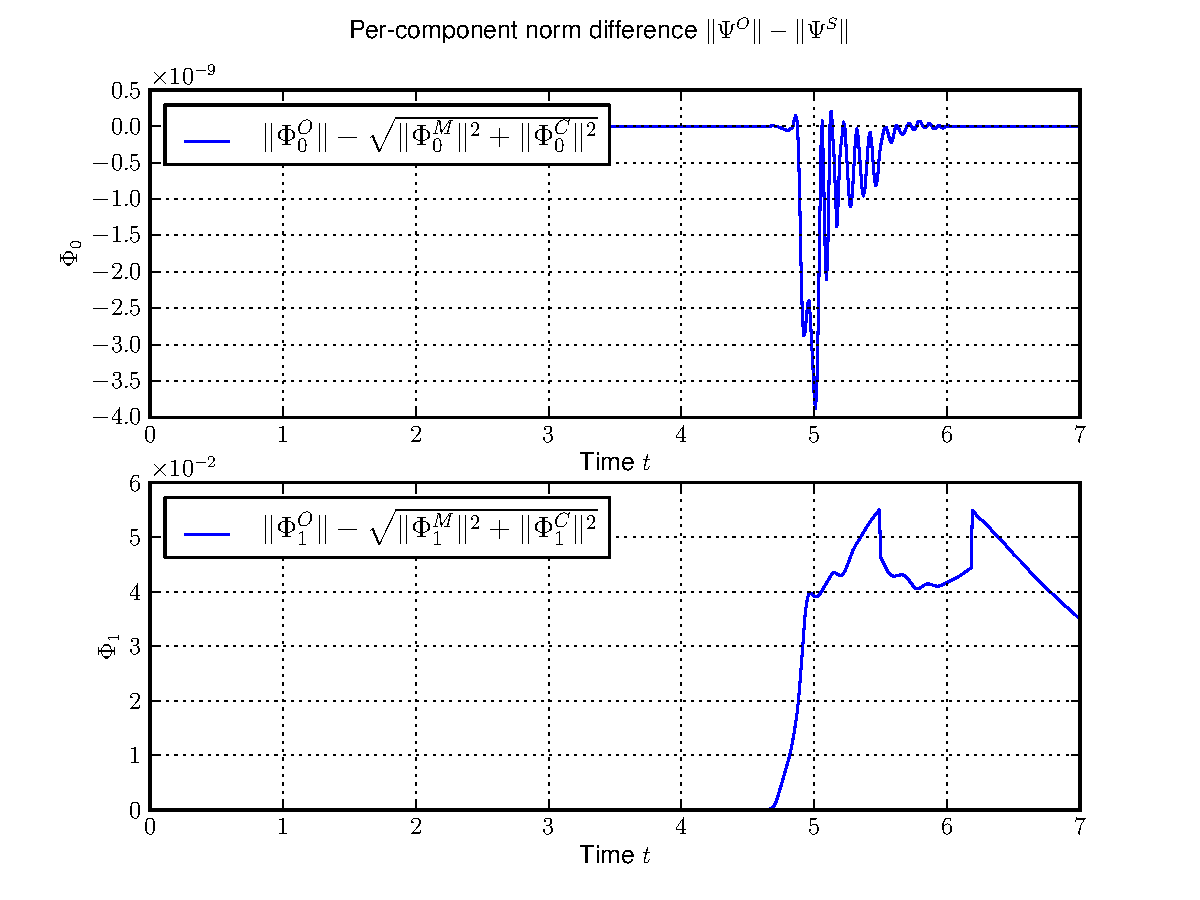
\includegraphics[width=0.5\linewidth]{./figures/delta_gap_spawn_phi2_k0/norms_compare_components_diff_group0.pdf}
  }
  \subfloat[][]{
    \label{fig:spawn_delta_gap_phi2_k2_norms_drift}
    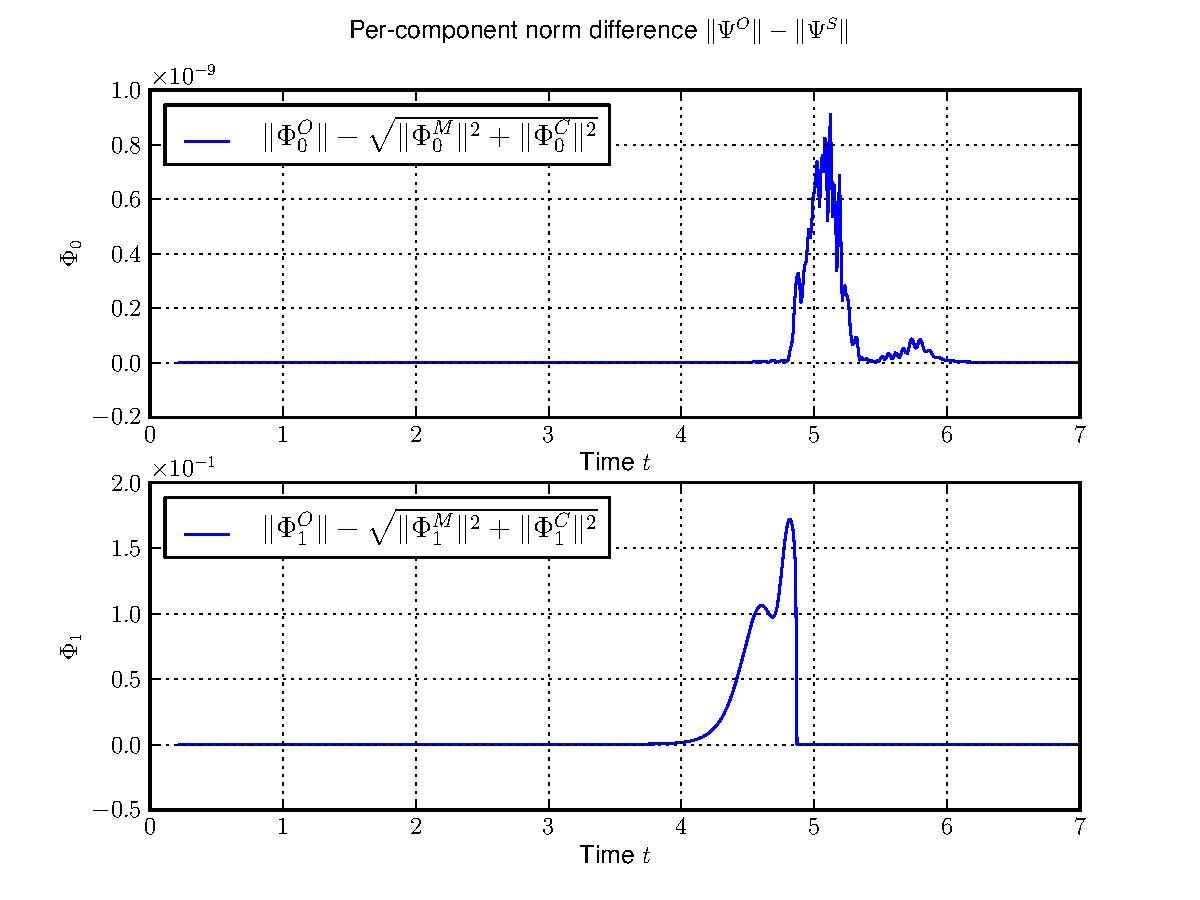
\includegraphics[width=0.5\linewidth]{./figures/delta_gap_spawn_phi2_k2/norms_compare_components_diff_group0.pdf}
  } \\
  \subfloat[][]{
    \label{fig:spawn_delta_gap_phi3_k0_norms_drift}
    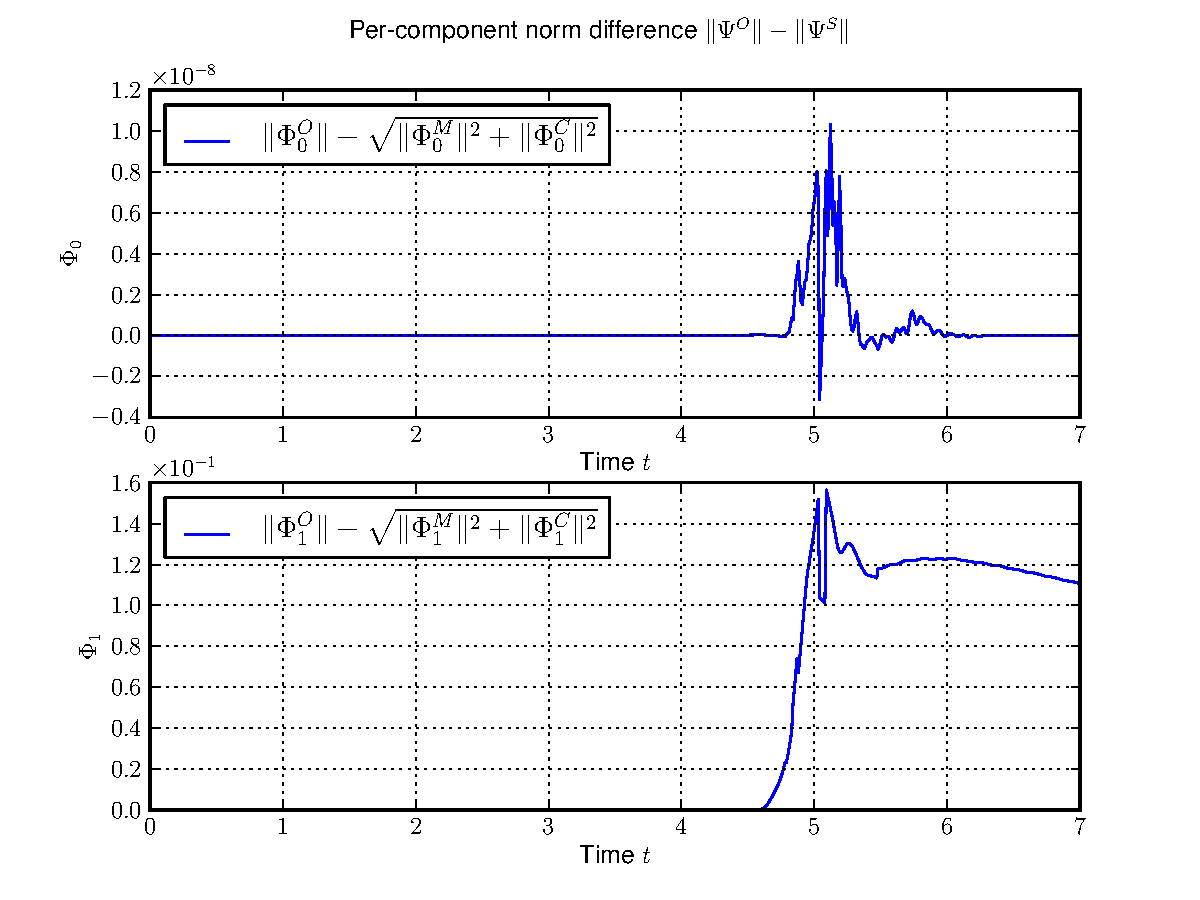
\includegraphics[width=0.5\linewidth]{./figures/delta_gap_spawn_phi3_k0/norms_compare_components_diff_group0.pdf}
  }
  \subfloat[][]{
    \label{fig:spawn_delta_gap_phi3_k3_norms_drift}
    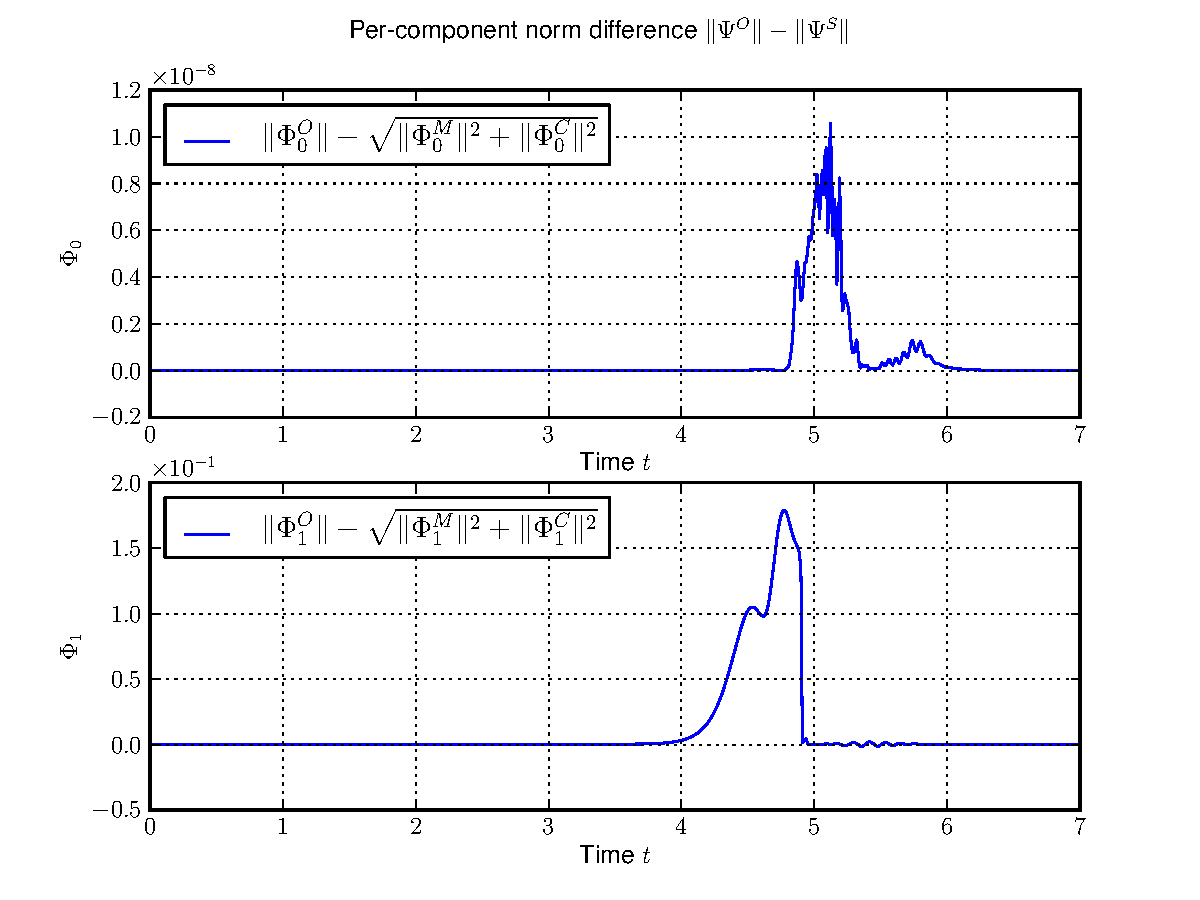
\includegraphics[width=0.5\linewidth]{./figures/delta_gap_spawn_phi3_k3/norms_compare_components_diff_group0.pdf}
  } \\
  \caption[The norm drift for several non-adiabatic examples]{
  This figure shows the component-wise drift in the norm for several non-adiabatic examples.
  The individual panels are for different wavepackets $\Psi = \phi_i$ and different
  values of $k$ where the $k$ is the one from formula \eqref{eq:estimate_abssqrPQ}.
  The full set of simulation parameters is printed in \ref{cfg:delta_gap_apost}.
  \subref{fig:spawn_delta_gap_phi1_k0_norms_drift} $\Psi = \phi_1$ and $k=0$
  \subref{fig:spawn_delta_gap_phi1_k1_norms_drift} $\Psi = \phi_1$ and $k=1$
  \subref{fig:spawn_delta_gap_phi2_k0_norms_drift} $\Psi = \phi_2$ and $k=0$
  \subref{fig:spawn_delta_gap_phi2_k2_norms_drift} $\Psi = \phi_2$ and $k=2$
  \subref{fig:spawn_delta_gap_phi3_k0_norms_drift} $\Psi = \phi_3$ and $k=0$
  \subref{fig:spawn_delta_gap_phi3_k3_norms_drift} $\Psi = \phi_3$ and $k=3$
  \label{fig:spawn_delta_gap_norms_drift1}
  }
\end{figure}


\begin{figure}[h!]
  \centering
  \subfloat[][]{
    \label{fig:spawn_delta_gap_phi4_k0_norms_drift}
    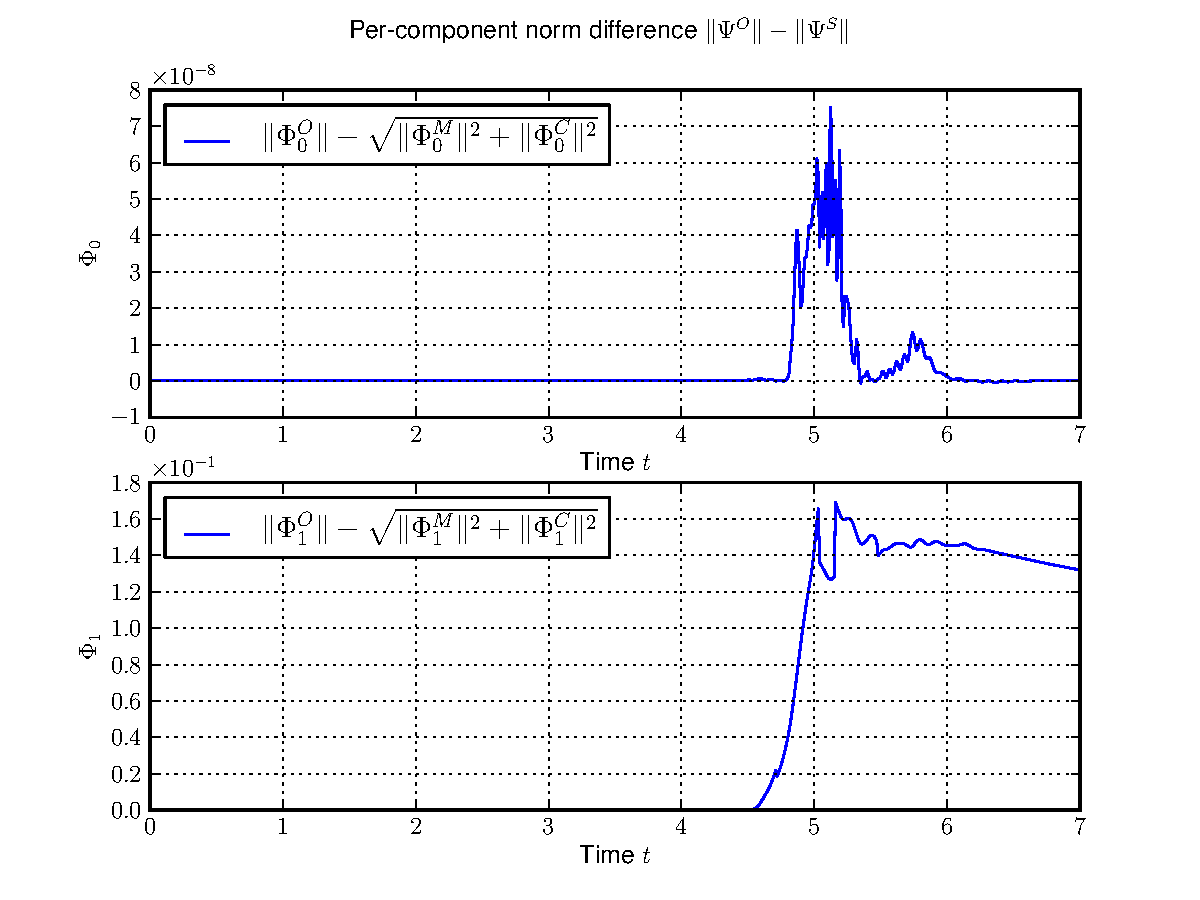
\includegraphics[width=0.5\linewidth]{./figures/delta_gap_spawn_phi4_k0/norms_compare_components_diff_group0.pdf}
  }
  \subfloat[][]{
    \label{fig:spawn_delta_gap_phi4_k4_norms_drift}
    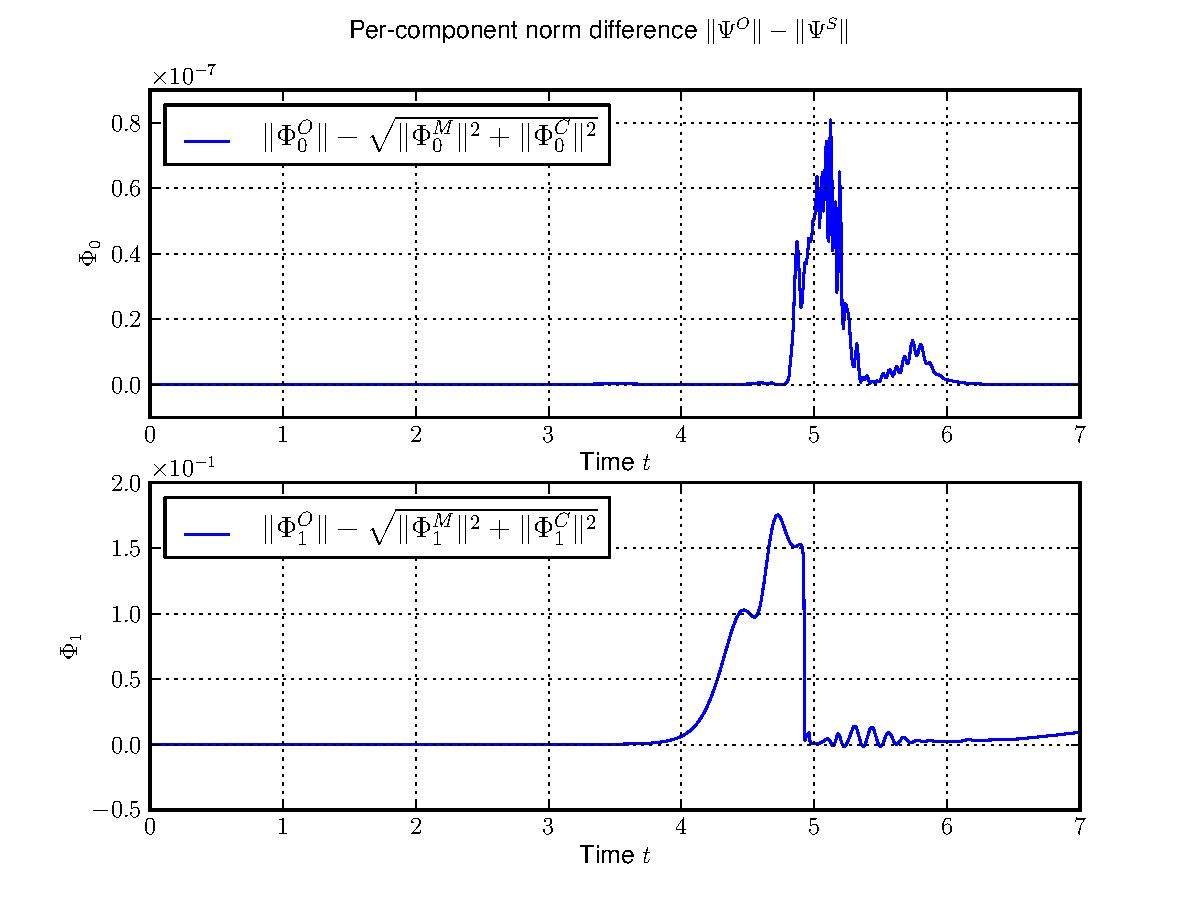
\includegraphics[width=0.5\linewidth]{./figures/delta_gap_spawn_phi4_k4/norms_compare_components_diff_group0.pdf}
  } \\
  \subfloat[][]{
    \label{fig:spawn_delta_gap_phi0phi1_k0_norms_drift}
    \includegraphics[width=0.5\linewidth]{./figures/delta_gap_spawn_phi0phi1_k0/norms_compare_components_diff_group0.pdf}
  }
  \subfloat[][]{
    \label{fig:spawn_delta_gap_phi2phi3_k0_norms_drift}
    \includegraphics[width=0.5\linewidth]{./figures/delta_gap_spawn_phi2phi3_k0/norms_compare_components_diff_group0.pdf}
  } \\
  \subfloat[][]{
    \label{fig:spawn_delta_gap_phi0_k0_norms_drift}
    \includegraphics[width=0.5\linewidth]{./figures/delta_gap_spawn_phi0_k0/norms_compare_components_diff_group0.pdf}
  } \\
  \caption[The norm drift for several non-adiabatic examples]{
  This figure shows the component-wise drift in the norm for several non-adiabatic examples.
  The individual panels are for different wavepackets $\Psi = \phi_i$ and different
  values of $k$ where the $k$ is the one from formula \eqref{eq:estimate_abssqrPQ}.
  The full set of simulation parameters is printed in \ref{cfg:delta_gap_apost}.
  \subref{fig:spawn_delta_gap_phi4_k0_norms_drift} $\Psi = \phi_4$ and $k=0$
  \subref{fig:spawn_delta_gap_phi4_k4_norms_drift} $\Psi = \phi_4$ and $k=4$
  \subref{fig:spawn_delta_gap_phi0phi1_k0_norms_drift} $\Psi = \phi_0 + \phi_1$ and $k=0$
  \subref{fig:spawn_delta_gap_phi2phi3_k0_norms_drift} $\Psi = \phi_2 + \phi_3$ and $k=0$
  \subref{fig:spawn_delta_gap_phi0_k0_norms_drift} $\Psi = \phi_0$ and $k=0$
  \label{fig:spawn_delta_gap_norms_drift2}
  }
\end{figure}



\begin{figure}[h!]
  \centering
  \subfloat[][]{
    \label{fig:spawn_delta_gap_phi1_k0_energies}
    \includegraphics[width=0.5\linewidth]{./figures/delta_gap_spawn_phi1_k0/energies_compare_components_group0.pdf}
  }
  \subfloat[][]{
    \label{fig:spawn_delta_gap_phi1_k1_energies}
    \includegraphics[width=0.5\linewidth]{./figures/delta_gap_spawn_phi1_k1/energies_compare_components_group0.pdf}
  } \\
  \subfloat[][]{
    \label{fig:spawn_delta_gap_phi2_k0_energies}
    \includegraphics[width=0.5\linewidth]{./figures/delta_gap_spawn_phi2_k0/energies_compare_components_group0.pdf}
  }
  \subfloat[][]{
    \label{fig:spawn_delta_gap_phi2_k2_energies}
    \includegraphics[width=0.5\linewidth]{./figures/delta_gap_spawn_phi2_k2/energies_compare_components_group0.pdf}
  } \\
  \subfloat[][]{
    \label{fig:spawn_delta_gap_phi3_k0_energies}
    \includegraphics[width=0.5\linewidth]{./figures/delta_gap_spawn_phi3_k0/energies_compare_components_group0.pdf}
  }
  \subfloat[][]{
    \label{fig:spawn_delta_gap_phi3_k3_energies}
    \includegraphics[width=0.5\linewidth]{./figures/delta_gap_spawn_phi3_k3/energies_compare_components_group0.pdf}
  } \\
  \caption[The kinetic and potential energies for several non-adiabatic examples]{
  This figure shows the kinetic and potential energies for several non-adiabatic examples.
  The individual panels are for different wavepackets $\Psi = \phi_i$ and different
  values of $k$ where the $k$ is the one from formula \eqref{eq:estimate_abssqrPQ}.
  The full set of simulation parameters is printed in \ref{cfg:delta_gap_apost}.
  \subref{fig:spawn_delta_gap_phi1_k0_energies} $\Psi = \phi_1$ and $k=0$
  \subref{fig:spawn_delta_gap_phi1_k1_energies} $\Psi = \phi_1$ and $k=1$
  \subref{fig:spawn_delta_gap_phi2_k0_energies} $\Psi = \phi_2$ and $k=0$
  \subref{fig:spawn_delta_gap_phi2_k2_energies} $\Psi = \phi_2$ and $k=2$
  \subref{fig:spawn_delta_gap_phi3_k0_energies} $\Psi = \phi_3$ and $k=0$
  \subref{fig:spawn_delta_gap_phi3_k3_energies} $\Psi = \phi_3$ and $k=3$
  \label{fig:spawn_delta_gap_energies1}
  }
\end{figure}


\begin{figure}[h!]
  \centering
  \subfloat[][]{
    \label{fig:spawn_delta_gap_phi4_k0_energies}
    \includegraphics[width=0.5\linewidth]{./figures/delta_gap_spawn_phi4_k0/energies_compare_components_group0.pdf}
  }
  \subfloat[][]{
    \label{fig:spawn_delta_gap_phi4_k4_energies}
    \includegraphics[width=0.5\linewidth]{./figures/delta_gap_spawn_phi4_k4/energies_compare_components_group0.pdf}
  } \\
  \subfloat[][]{
    \label{fig:spawn_delta_gap_phi0phi1_k0_energies}
    \includegraphics[width=0.5\linewidth]{./figures/delta_gap_spawn_phi0phi1_k0/energies_compare_components_group0.pdf}
  }
  \subfloat[][]{
    \label{fig:spawn_delta_gap_phi2phi3_k0_energies}
    \includegraphics[width=0.5\linewidth]{./figures/delta_gap_spawn_phi2phi3_k0/energies_compare_components_group0.pdf}
  } \\
  \subfloat[][]{
    \label{fig:spawn_delta_gap_phi0_k0_energies}
    \includegraphics[width=0.5\linewidth]{./figures/delta_gap_spawn_phi0_k0/energies_compare_components_group0.pdf}
  } \\
  \caption[The kinetic and potential energies for several non-adiabatic examples]{
  This figure shows the kinetic and potential energies for several non-adiabatic examples.
  The individual panels are for different wavepackets $\Psi = \phi_i$ and different
  values of $k$ where the $k$ is the one from formula \eqref{eq:estimate_abssqrPQ}.
  The full set of simulation parameters is printed in \ref{cfg:delta_gap_apost}.
  \subref{fig:spawn_delta_gap_phi4_k0_energies} $\Psi = \phi_4$ and $k=0$
  \subref{fig:spawn_delta_gap_phi4_k4_energies} $\Psi = \phi_4$ and $k=4$
  \subref{fig:spawn_delta_gap_phi0phi1_k0_energies} $\Psi = \phi_0 + \phi_1$ and $k=0$
  \subref{fig:spawn_delta_gap_phi2phi3_k0_energies} $\Psi = \phi_2 + \phi_3$ and $k=0$
  \subref{fig:spawn_delta_gap_phi0_k0_energies} $\Psi = \phi_0$ and $k=0$
  \label{fig:spawn_delta_gap_energies2}
  }
\end{figure}



\begin{figure}[h!]
  \centering
  \subfloat[][]{
    \label{fig:spawn_delta_gap_phi1_k0_energy_drift}
    \includegraphics[width=0.5\linewidth]{./figures/delta_gap_spawn_phi1_k0/energies_compare_components_diff_group0.pdf}
  }
  \subfloat[][]{
    \label{fig:spawn_delta_gap_phi1_k1_energy_drift}
    \includegraphics[width=0.5\linewidth]{./figures/delta_gap_spawn_phi1_k1/energies_compare_components_diff_group0.pdf}
  } \\
  \subfloat[][]{
    \label{fig:spawn_delta_gap_phi2_k0_energy_drift}
    \includegraphics[width=0.5\linewidth]{./figures/delta_gap_spawn_phi2_k0/energies_compare_components_diff_group0.pdf}
  }
  \subfloat[][]{
    \label{fig:spawn_delta_gap_phi2_k2_energy_drift}
    \includegraphics[width=0.5\linewidth]{./figures/delta_gap_spawn_phi2_k2/energies_compare_components_diff_group0.pdf}
  } \\
  \subfloat[][]{
    \label{fig:spawn_delta_gap_phi3_k0_energy_drift}
    \includegraphics[width=0.5\linewidth]{./figures/delta_gap_spawn_phi3_k0/energies_compare_components_diff_group0.pdf}
  }
  \subfloat[][]{
    \label{fig:spawn_delta_gap_phi3_k3_energy_drift}
    \includegraphics[width=0.5\linewidth]{./figures/delta_gap_spawn_phi3_k3/energies_compare_components_diff_group0.pdf}
  } \\
  \caption[The drift in the kinetic, potential and overall energy for several non-adiabatic examples]{
  This figure shows the drift in the kinetic, potential and overall energy for
  several non-adiabatic examples. The individual panels are for different wavepackets $\Psi = \phi_i$
  and different values of $k$ where the $k$ is the one from formula \eqref{eq:estimate_abssqrPQ}.
  The full set of simulation parameters is printed in \ref{cfg:delta_gap_apost}.
  \subref{fig:spawn_delta_gap_phi1_k0_energy_drift} $\Psi = \phi_1$ and $k=0$
  \subref{fig:spawn_delta_gap_phi1_k1_energy_drift} $\Psi = \phi_1$ and $k=1$
  \subref{fig:spawn_delta_gap_phi2_k0_energy_drift} $\Psi = \phi_2$ and $k=0$
  \subref{fig:spawn_delta_gap_phi2_k2_energy_drift} $\Psi = \phi_2$ and $k=2$
  \subref{fig:spawn_delta_gap_phi3_k0_energy_drift} $\Psi = \phi_3$ and $k=0$
  \subref{fig:spawn_delta_gap_phi3_k3_energy_drift} $\Psi = \phi_3$ and $k=3$
  \label{fig:spawn_delta_gap_energy_drift1}
  }
\end{figure}


\begin{figure}[h!]
  \centering
  \subfloat[][]{
    \label{fig:spawn_delta_gap_phi4_k0_energy_drift}
    \includegraphics[width=0.5\linewidth]{./figures/delta_gap_spawn_phi4_k0/energies_compare_components_diff_group0.pdf}
  }
  \subfloat[][]{
    \label{fig:spawn_delta_gap_phi4_k4_energy_drift}
    \includegraphics[width=0.5\linewidth]{./figures/delta_gap_spawn_phi4_k4/energies_compare_components_diff_group0.pdf}
  } \\
  \subfloat[][]{
    \label{fig:spawn_delta_gap_phi0phi1_k0_energy_drift}
    \includegraphics[width=0.5\linewidth]{./figures/delta_gap_spawn_phi0phi1_k0/energies_compare_components_diff_group0.pdf}
  }
  \subfloat[][]{
    \label{fig:spawn_delta_gap_phi2phi3_k0_energy_drift}
    \includegraphics[width=0.5\linewidth]{./figures/delta_gap_spawn_phi2phi3_k0/energies_compare_components_diff_group0.pdf}
  } \\
  \subfloat[][]{
    \label{fig:spawn_delta_gap_phi0_k0_energy_drift}
    \includegraphics[width=0.5\linewidth]{./figures/delta_gap_spawn_phi0_k0/energies_compare_components_diff_group0.pdf}
  } \\
  \caption[The drift in the kinetic, potential and overall energy for several non-adiabatic examples]{
  This figure shows the drift in the kinetic, potential and overall energy for
  several non-adiabatic examples. The individual panels are for different wavepackets $\Psi = \phi_i$
  and different values of $k$ where the $k$ is the one from formula \eqref{eq:estimate_abssqrPQ}.
  The full set of simulation parameters is printed in \ref{cfg:delta_gap_apost}.
  \subref{fig:spawn_delta_gap_phi4_k0_energy_drift} $\Psi = \phi_4$ and $k=0$
  \subref{fig:spawn_delta_gap_phi4_k4_energy_drift} $\Psi = \phi_4$ and $k=4$
  \subref{fig:spawn_delta_gap_phi0phi1_k0_energy_drift} $\Psi = \phi_0 + \phi_1$ and $k=0$
  \subref{fig:spawn_delta_gap_phi2phi3_k0_energy_drift} $\Psi = \phi_2 + \phi_3$ and $k=0$
  \subref{fig:spawn_delta_gap_phi0_k0_energy_drift} $\Psi = \phi_0$ and $k=0$
  \label{fig:spawn_delta_gap_energy_drift2}
  }
\end{figure}



\begin{figure}[h!]
  \centering
  \subfloat[][]{
    \label{fig:spawn_delta_gap_phi1_k0_pqcond}
    \includegraphics[width=0.4\linewidth]{./figures/delta_gap_spawn_phi1_k0/conjQP-conjPQ_block1.pdf}
  }
  \subfloat[][]{
    \label{fig:spawn_delta_gap_phi1_k1_pqcond}
    \includegraphics[width=0.4\linewidth]{./figures/delta_gap_spawn_phi1_k1/conjQP-conjPQ_block1.pdf}
  } \\
  \subfloat[][]{
    \label{fig:spawn_delta_gap_phi2_k0_pqcond}
    \includegraphics[width=0.4\linewidth]{./figures/delta_gap_spawn_phi2_k0/conjQP-conjPQ_block1.pdf}
  }
  \subfloat[][]{
    \label{fig:spawn_delta_gap_phi2_k2_pqcond}
    \includegraphics[width=0.4\linewidth]{./figures/delta_gap_spawn_phi2_k2/conjQP-conjPQ_block1.pdf}
  } \\
  \subfloat[][]{
    \label{fig:spawn_delta_gap_phi3_k0_pqcond}
    \includegraphics[width=0.4\linewidth]{./figures/delta_gap_spawn_phi3_k0/conjQP-conjPQ_block1.pdf}
  }
  \subfloat[][]{
    \label{fig:spawn_delta_gap_phi3_k3_pqcond}
    \includegraphics[width=0.4\linewidth]{./figures/delta_gap_spawn_phi3_k3/conjQP-conjPQ_block1.pdf}
  } \\
  \caption[Violation of the condition \eqref{eq:symplecticity_condition} for $k>0$]{
  This figure shows that the symplecticity condition from equation \eqref{eq:symplecticity_condition}
  is violated for the simulations with $k>0$. The reason for this is not that $k>0$ but
  is described in detail at the end of chapter \ref{ch:spawnprocedure}. Luckily
  for us the violations never happened during or after the avoided crossing.
  The values in the left panels are numerically zero up to machine precision.
  The full set of simulation parameters is printed in \ref{cfg:delta_gap_apost}.
  \subref{fig:spawn_delta_gap_phi1_k0_pqcond} $\Psi = \phi_1$ and $k=0$
  \subref{fig:spawn_delta_gap_phi1_k1_pqcond} $\Psi = \phi_1$ and $k=1$
  \subref{fig:spawn_delta_gap_phi2_k0_pqcond} $\Psi = \phi_2$ and $k=0$
  \subref{fig:spawn_delta_gap_phi2_k2_pqcond} $\Psi = \phi_2$ and $k=2$
  \subref{fig:spawn_delta_gap_phi3_k0_pqcond} $\Psi = \phi_3$ and $k=0$
  \subref{fig:spawn_delta_gap_phi3_k3_pqcond} $\Psi = \phi_3$ and $k=3$
  \label{fig:spawn_delta_gap_spawn_pqcond1}
  }
\end{figure}


The two figures \ref{fig:spawn_delta_gap_spawn_errors1} and
\ref{fig:spawn_delta_gap_spawn_errors2} show the spawn error. We see that with
the matching choice of $k$ we have a spawn error that is about an order of magnitude
smaller than what we get with $k=0$. Thus it is important to use the correct $k$ in
formula \eqref{eq:estimate_abssqrPQ}. As an example if we start with a $\phi_3$
we must set $k=3$ for obtaining good results. For sure we could reduce the error
further if we choose a larger basis size $\eta$ but this is not the point here.
All comparisons were done with a basis size of $\eta = 16$ and $\mu = \eta$.

\begin{figure}[h!]
  \centering
  \subfloat[][]{
    \label{fig:spawn_delta_gap_phi1_k0}
    \includegraphics[width=0.5\linewidth]{./figures/delta_gap_spawn_phi1_k0/spawn_error_component_norms.pdf}
  }
  \subfloat[][]{
    \label{fig:spawn_delta_gap_phi1_k1}
    \includegraphics[width=0.5\linewidth]{./figures/delta_gap_spawn_phi1_k1/spawn_error_component_norms.pdf}
  } \\
  \subfloat[][]{
    \label{fig:spawn_delta_gap_phi2_k0}
    \includegraphics[width=0.5\linewidth]{./figures/delta_gap_spawn_phi2_k0/spawn_error_component_norms.pdf}
  }
  \subfloat[][]{
    \label{fig:spawn_delta_gap_phi2_k2}
    \includegraphics[width=0.5\linewidth]{./figures/delta_gap_spawn_phi2_k2/spawn_error_component_norms.pdf}
  } \\
  \subfloat[][]{
    \label{fig:spawn_delta_gap_phi3_k0}
    \includegraphics[width=0.5\linewidth]{./figures/delta_gap_spawn_phi3_k0/spawn_error_component_norms.pdf}
  }
  \subfloat[][]{
    \label{fig:spawn_delta_gap_phi3_k3}
    \includegraphics[width=0.5\linewidth]{./figures/delta_gap_spawn_phi3_k3/spawn_error_component_norms.pdf}
  } \\
  \caption[Spawning error in the $L^2$ and maximum norm for a non-adiabatic example]{
  This figure shows the spawn error $\| \Psi - (\tilde{v} + \tilde{w})\|$ for both
  components in $L^2$ norm (blue) and maximum norm (green). The individual panels are
  for different wavepackets $\Psi = \phi_i$ and different values of $k$ where the $k$ is
  the one from formula \eqref{eq:estimate_abssqrPQ}.
  The full set of simulation parameters is printed in \ref{cfg:delta_gap_apost}.
  \subref{fig:spawn_delta_gap_phi1_k0} $\Psi = \phi_1$ and $k=0$
  \subref{fig:spawn_delta_gap_phi1_k1} $\Psi = \phi_1$ and $k=1$
  \subref{fig:spawn_delta_gap_phi2_k0} $\Psi = \phi_2$ and $k=0$
  \subref{fig:spawn_delta_gap_phi2_k2} $\Psi = \phi_2$ and $k=2$
  \subref{fig:spawn_delta_gap_phi3_k0} $\Psi = \phi_3$ and $k=0$
  \subref{fig:spawn_delta_gap_phi3_k3} $\Psi = \phi_3$ and $k=3$
  \label{fig:spawn_delta_gap_spawn_errors1}
  }
\end{figure}


\begin{figure}[h!]
  \centering
  \subfloat[][]{
    \label{fig:spawn_delta_gap_phi4_k0}
    \includegraphics[width=0.5\linewidth]{./figures/delta_gap_spawn_phi4_k0/spawn_error_component_norms.pdf}
  }
  \subfloat[][]{
    \label{fig:spawn_delta_gap_phi4_k4}
    \includegraphics[width=0.5\linewidth]{./figures/delta_gap_spawn_phi4_k4/spawn_error_component_norms.pdf}
  } \\
  \subfloat[][]{
    \label{fig:spawn_delta_gap_phi0phi1_k0}
    \includegraphics[width=0.5\linewidth]{./figures/delta_gap_spawn_phi0phi1_k0/spawn_error_component_norms.pdf}
  }
  \subfloat[][]{
    \label{fig:spawn_delta_gap_phi2phi3_k0}
    \includegraphics[width=0.5\linewidth]{./figures/delta_gap_spawn_phi2phi3_k0/spawn_error_component_norms.pdf}
  } \\
  \subfloat[][]{
    \label{fig:spawn_delta_gap_phi0_k0}
    \includegraphics[width=0.5\linewidth]{./figures/delta_gap_spawn_phi0_k0/spawn_error_component_norms.pdf}
  } \\
  \caption[Spawning error in the $L^2$ and maximum norm for a non-adiabatic example]{
  This figure shows the spawn error $\| \Psi - (\tilde{v} + \tilde{w})\|$ for both
  components in $L^2$ norm (blue) and maximum norm (green). The individual panels are
  for different wavepackets $\Psi = \phi_i$ and different values of $k$ where the $k$ is
  the one from formula \eqref{eq:estimate_abssqrPQ}.
  The full set of simulation parameters is printed in \ref{cfg:delta_gap_apost}.
  \subref{fig:spawn_delta_gap_phi4_k0} $\Psi = \phi_4$ and $k=0$
  \subref{fig:spawn_delta_gap_phi4_k4} $\Psi = \phi_4$ and $k=4$
  \subref{fig:spawn_delta_gap_phi0phi1_k0} $\Psi = \phi_0 + \phi_1$ and $k=0$
  \subref{fig:spawn_delta_gap_phi2phi3_k0} $\Psi = \phi_2 + \phi_3$ and $k=0$
  \subref{fig:spawn_delta_gap_phi0_k0} $\Psi = \phi_0$ and $k=0$
  \label{fig:spawn_delta_gap_spawn_errors2}
  }
\end{figure}


\FloatBarrier
\section{Spawning and propagation}

The combination of spawning and propagation in the non-adiabatic case is similar
to what is shown in section \ref{sec:spawn_propag_tunnel}. But the small differences
justify the review of the algorithm in the current section. We use the same basic
notations from section \ref{sec:theoretical_basis_na}. The potential has $N$ energy
levels and hence the wavepacket has $N$ components. The wavepacket is usually assumed
to be homogeneous but this is not necessary. (In the case of inhomogeneous
wavepackets we can forget about the characteristic component $\chi$.)

We start with a single wavepacket $\Ket{\Psi}$ as initial value at time $\tau_0$
and assume that the spawning criterion is fulfilled only once during the whole simulation.
Then we will end up with two wavepackets $\Ket{\Psi_0}$ and $\Ket{\Psi_1}$ after
spawning. There are basis transformations between the canonical and the eigenbasis
involved and we denote quantities in the corresponding basis with a $c$ or $e$
superscript. These transformations albeit expensive are necessary as the propagation
takes place in the canonical basis but we have to run the whole spawning procedure
in the eigenbasis where the different components are decoupled. The transformation
matrix $M$ was defined in section \ref{sec:diagonalize_potential}.

\begin{algorithm}
\caption{Spawning propagation method (simplified non-adiabatic case)}
\label{al:spawning_propagation_na_simplified}
\begin{algorithmic}
  \REQUIRE A series $t$ consisting of timesteps $\{\tau_0, \ldots, \tau_{\text{max}}\}$
  \REQUIRE The potential $V\ofs{x}$
  \REQUIRE The initial (homogeneous) wavepacket $\Ket{\Psi^c\ofs{t=\tau_o}}$
  \REQUIRE The monitored component $0 \leq \nu \leq N-1$
  \REQUIRE The value of $0 \leq k \leq K-1$
  \REQUIRE A spawn threshold $\tau$
  \FORALL{$\tau_i \in t$}
    \STATE // Transform the packet to the eigenbasis
    \STATE $\Psi^e \assign M^{-1} \Psi^c$
    \STATE // Extract the monitored component $\Phi_\nu$ of $\Psi^e$
    \STATE $w \assign \Phi_\nu = \sum_{k=0}^{K-1} c^\nu_k \phi_k$
    \STATE // Check the spawning criterion
    \IF{$\Braket{w|w} \geq \tau^2$}
      \STATE // Perform spawning procedure
      \STATE // Estimate the parameters of the fragment by algorithm \ref{al:parameter_estimation}
      \STATE $\tilde{\Pi} \assign \textbf{estimate\_parameters}(w)$
      \STATE // Move the fragment $w$ to the new basis by either algorithm \ref{al:lumping_method} or \ref{al:projection_method}
      \STATE $\tilde{w} \assign \textbf{change\_basis}(\tilde{\Pi}, w)$
      \STATE // Update the reminder (included in algorithm \ref{al:lumping_method} and \ref{al:projection_method})
      \STATE $\tilde{v} \assign \textbf{update\_remainder}(v, \tilde{w})$
      \STATE // We have now two new, full wavepackets
      \STATE $\Psi_0 \assign \left(\Phi_0, \ldots, \Phi_{\nu-1}, \Phi_\nu\assign\tilde{v}, \Phi_{\nu+1}, \ldots, \Phi_{N-1}\right)$
      \STATE $\Psi_1 \assign \left(0, \ldots, 0, \Phi_\nu\assign\tilde{w}, 0, \ldots, 0\right)$
      \STATE // Set the characteristic level $\chi$ of $\Psi_1$ to $\nu$
      \STATE // Only used for propagation with homogeneous wavepackets
      \STATE $\chi_{\Psi_1} \assign \nu$
      \STATE // Transform the packets back into the canonical basis
      \STATE $\Psi^c_0 \assign M \Psi^e_0$ and $\Psi^c_1 \assign M \Psi^e_1$
    \ENDIF
    \STATE // Time propagation of all $\Psi_j$ using the algorithms from \cite{FGL_semiclassical_dynamics} and \cite{BGH_natac}
    \FORALL{$\Psi_j\ofs{t=\tau_i}$}
       \STATE $\Psi_j\ofs{t=\tau_{i+1}} \assign \textbf{time\_propagation}(V, \Psi_j\ofs{t=\tau_i})$
    \ENDFOR
  \ENDFOR
\end{algorithmic}
\end{algorithm}

With algorithm \ref{al:spawning_propagation_na_simplified} we conclude this
chapter about spawning in the non-adiabatic case.

\end{chapter}
